\chapter{Electromagnetic shower shapes correction }
	\label{ch::sshapes}
	The chapter considers the electromagnetic shower development in the ATLAS \gls{emc} and its role in particle identification (ID). The existing mismodelling of the shower development in the Monte-Carlo simulation causes discrepancies in electron ID. A correction method that allows to achieve good correspondence between the data and the simulation is proposed, implemented and tested.
  \section{Introduction}
  The design and functionality of the ATLAS electromagnetic calorimeter was described in \ref{emc}. Let's consider a bit more in detail the physical processes happening in the \gls{emc}. 
  
  It order to measure particle's energy within the calorimeter we must make the particle to loose its entire energy within the calorimeter. For the electrons and photons with energies over few MeV (which is the case for the ATLAS experiment) the primary energy loss mechanism lies in bremsstrahlung radiation and pair creation. The two processes complete each other, so when a high-energy electron or photon gets into the calorimeter, it creates an avalanche-like process called the electromagnetic shower when a bremsstrahlung-radiated photons create more electron-positron pairs which in turn radiate more bremsstrahlung photons and so on and so forth (see Fig. \ref{fig::em_shower}.)\\
  	\begin{figure}[htbp]
  	\begin{subfigure}[t]{0.5\textwidth}
  		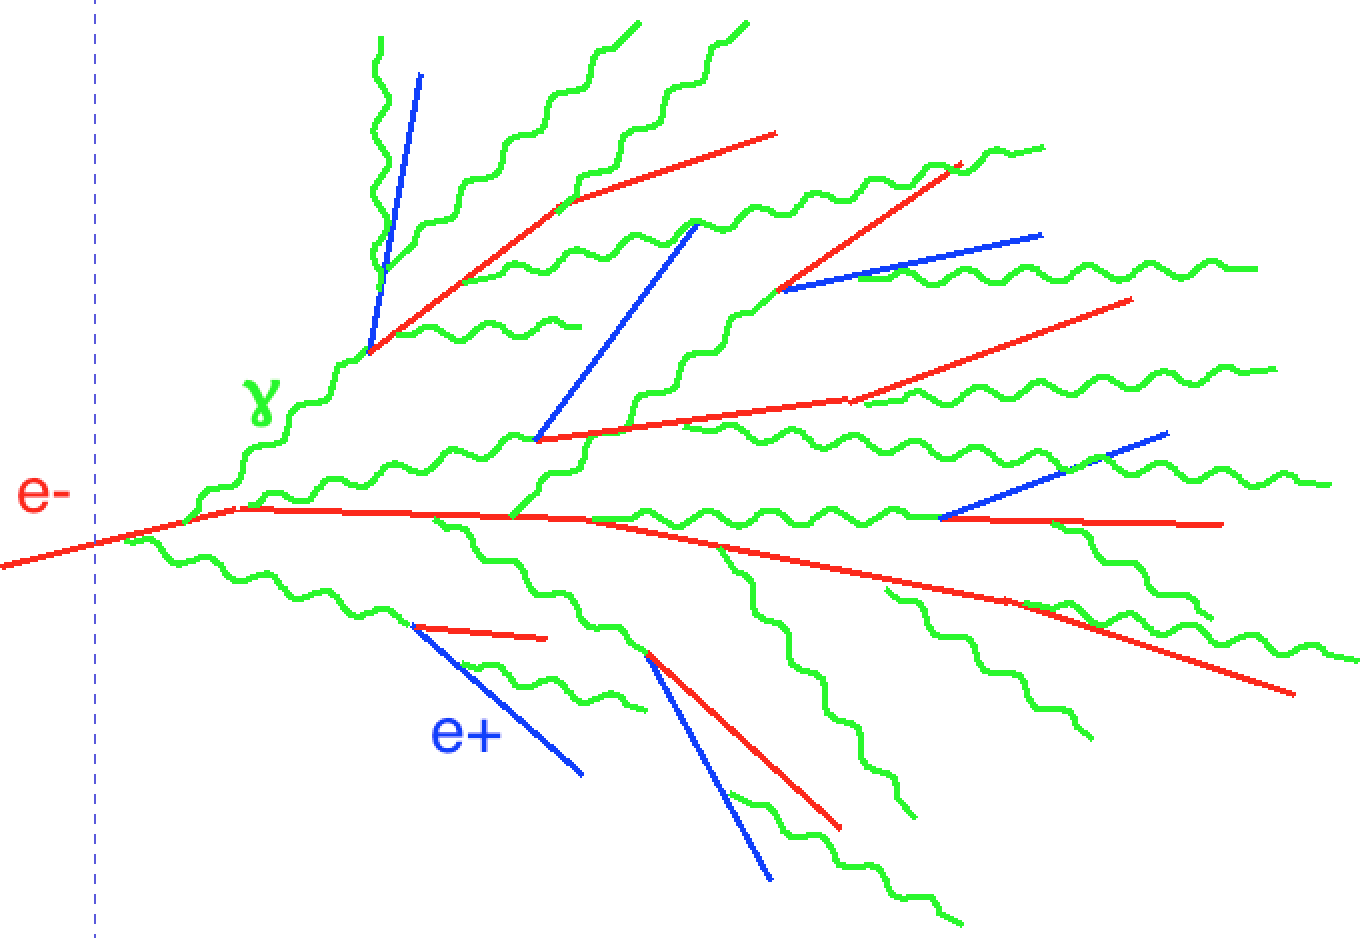
\includegraphics[width=\textwidth,keepaspectratio]{em_shower.png}
  		\caption[Started by an electron]{Initiated by an electron}
  		\label{fig::id}
  	\end{subfigure}
  	\hfill
  	\begin{subfigure}[t]{0.5\textwidth} 
  		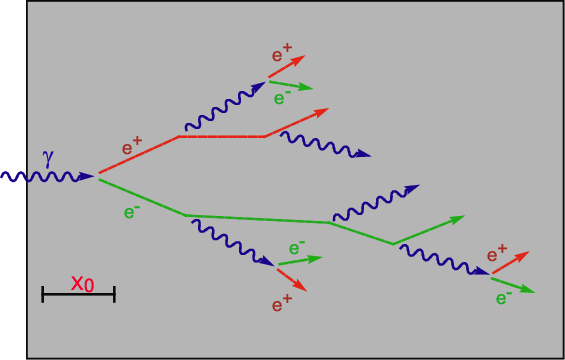
\includegraphics[width=\textwidth,keepaspectratio]{emshower.png}
  		\caption[Started by a $\gamma$-photon]{Initiated by a $\gamma$-photon}
  		\label{fig::pd}
  	\end{subfigure}
  	\caption{The schematic portrayal of EM shower development}
  	\label{fig::em_shower}
  \end{figure}
    The longitudinal and transverse development of the shower depends on the type of the initial particle and on its energy. The energy is well measured by the calorimeter, but identifying the particle still remains a challenging task. The transverse granularity of the ATLAS calorimeter allows to resolve the energy distribution within the electromagnetic shower in the transverse plane. This information can later be used for particle identification.
    
  When an e/$\gamma$ particle hits the calorimeter its footprint in the second layer of the calorimeter is visible as a cluster of calorimeter cells centered at the central cell having the most energy deposited (sometimes referred to as "the hottest cell"). Roughly 90$\%$ of shower energy is contained in the core 3x3 cells.  We have considered a cluster of 7x11 ($\eta$ x $\phi$) cells, which is schematically depicted on Fig. \ref{fig::profile_log}.
  
  
    	\begin{figure}[htbp]
  	\begin{subfigure}[t]{0.5\textwidth}
  		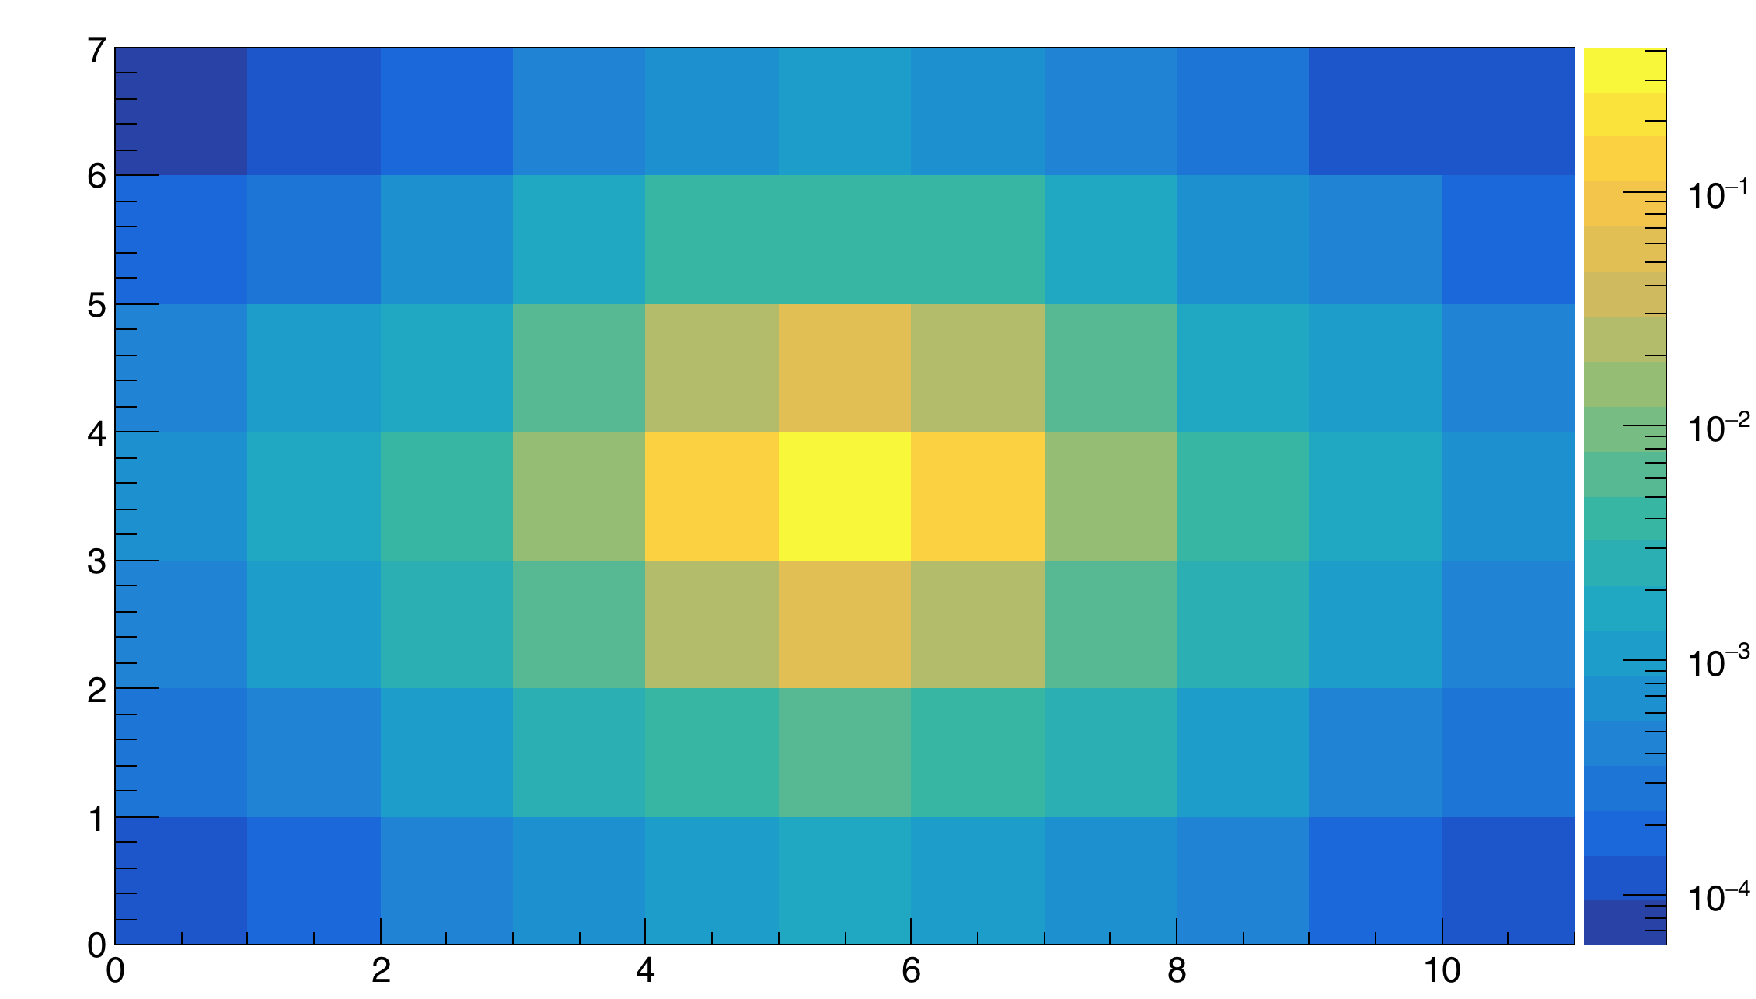
\includegraphics[width=\textwidth,keepaspectratio]{logscale.pdf}
  		\caption{Energy profile of a window of 7x11 cells in the 2nd calorimeter layer (logarithmic scale)}
  		\label{fig::profile_log}
  	\end{subfigure}
  	\hfill
  	\begin{subfigure}[t]{0.5\textwidth} 
  		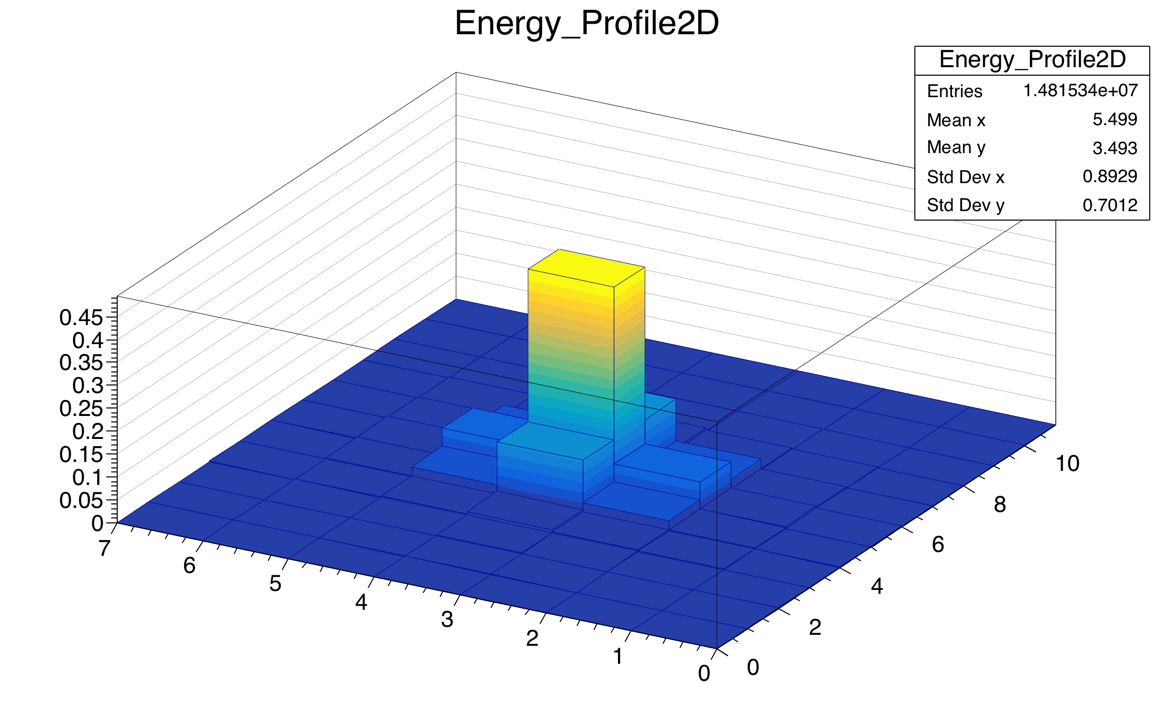
\includegraphics[width=\textwidth,keepaspectratio]{2dProfile.png}
  		\caption{2D profile of the cluster}
  		\label{fig::2d_profile}
  	\end{subfigure}
  	\caption{Visualisations of the 7x11 calorimeter cluster}
  	\label{fig::profiles}
  \end{figure}
  
  In order to characterise the energy distribution within the shower profile a number of observables called shower shapes are used. They are then used as an input for particle identification MVA algorithm. Current study focuses on the second layer of the calorimeter for which there are three shower shape observables described below \cite{egamma_perf_2017}:
  
    	\begin{figure}[htbp]
  	\begin{subfigure}[t]{0.4\textwidth}
  		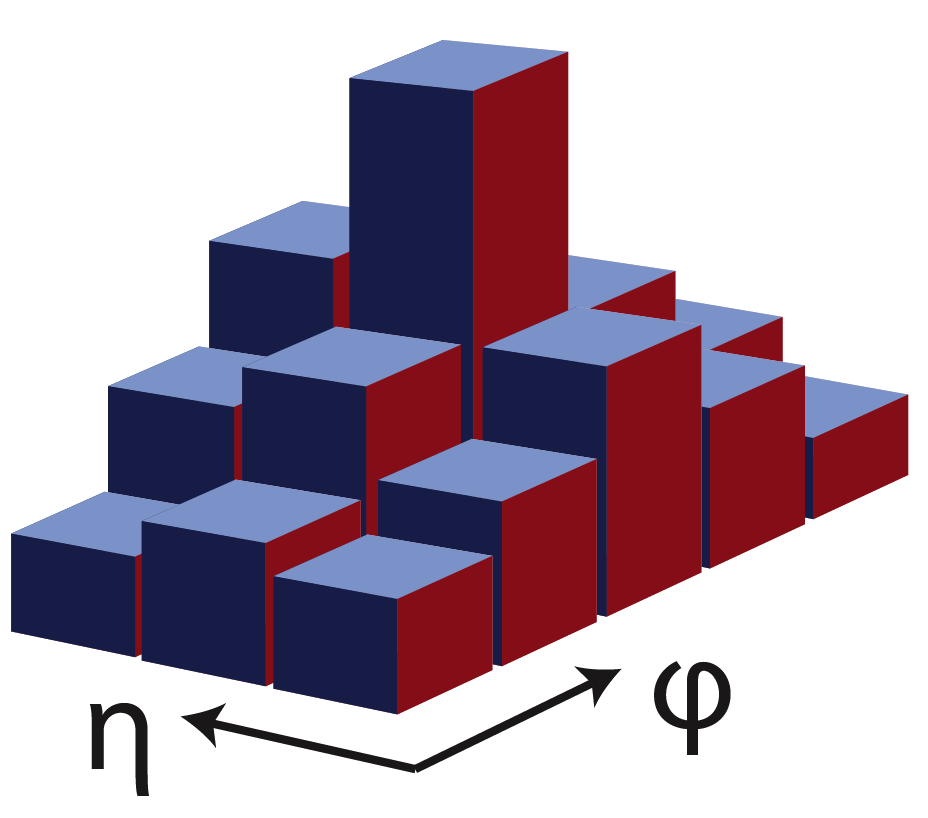
\includegraphics[width=\textwidth,keepaspectratio]{Weta2.png}
  		\caption[Lateral shower width $W_{\eta} 2$]{Lateral shower width $W_{\eta} 2$}
  		\label{fig::weta2}
  	\end{subfigure}
  	\hfill
  	\begin{subfigure}[t]{0.25\textwidth} 
  		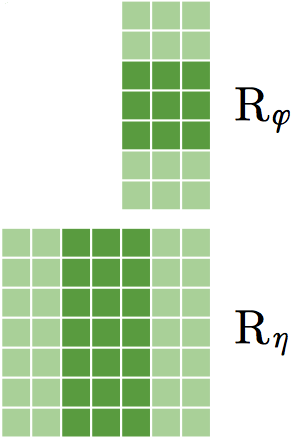
\includegraphics[width=\textwidth,keepaspectratio]{reta_rphi.png}
  		\caption[$R_{\phi}$ and $R_{\eta}$]{$R_{\phi}$ and $R_{\eta}$}
  		\label{fig::reta_rphi}
  	\end{subfigure}
  	\caption{Shower shapes in the second layer of the electromagnetic calorimeter}
  	\label{fig::sshapes}
  \end{figure}
  
  \begin{itemize}
  	\item Lateral shower width $W_{\eta 2} = \sqrt{\sum(E_i \eta^{2}_{i})-(\sum(E_i \eta_{i})/\sum(E_i))^2}$ calculated within a window of 3x5 cells.
  	\item $R_{\phi}$ - ratio of the energy in 3x3 cells over the energy in 3x7 cells centered around the hottest cell.
  	\item $R_{\eta}$ - ratio of the energy in 3x7 cells over the energy in 7x7 cells centered around the hottest cell.
  \end{itemize}
  
  The shower shapes distributions for different types of particles is shown in Fig. \ref{fig::sshapes_simul} - although the distributions overlap, combining the shower shapes information with the inputs from other detectors allow to identify the particle.  
    	\begin{figure}[htbp]
	\begin{subfigure}[t]{0.4\textwidth}
		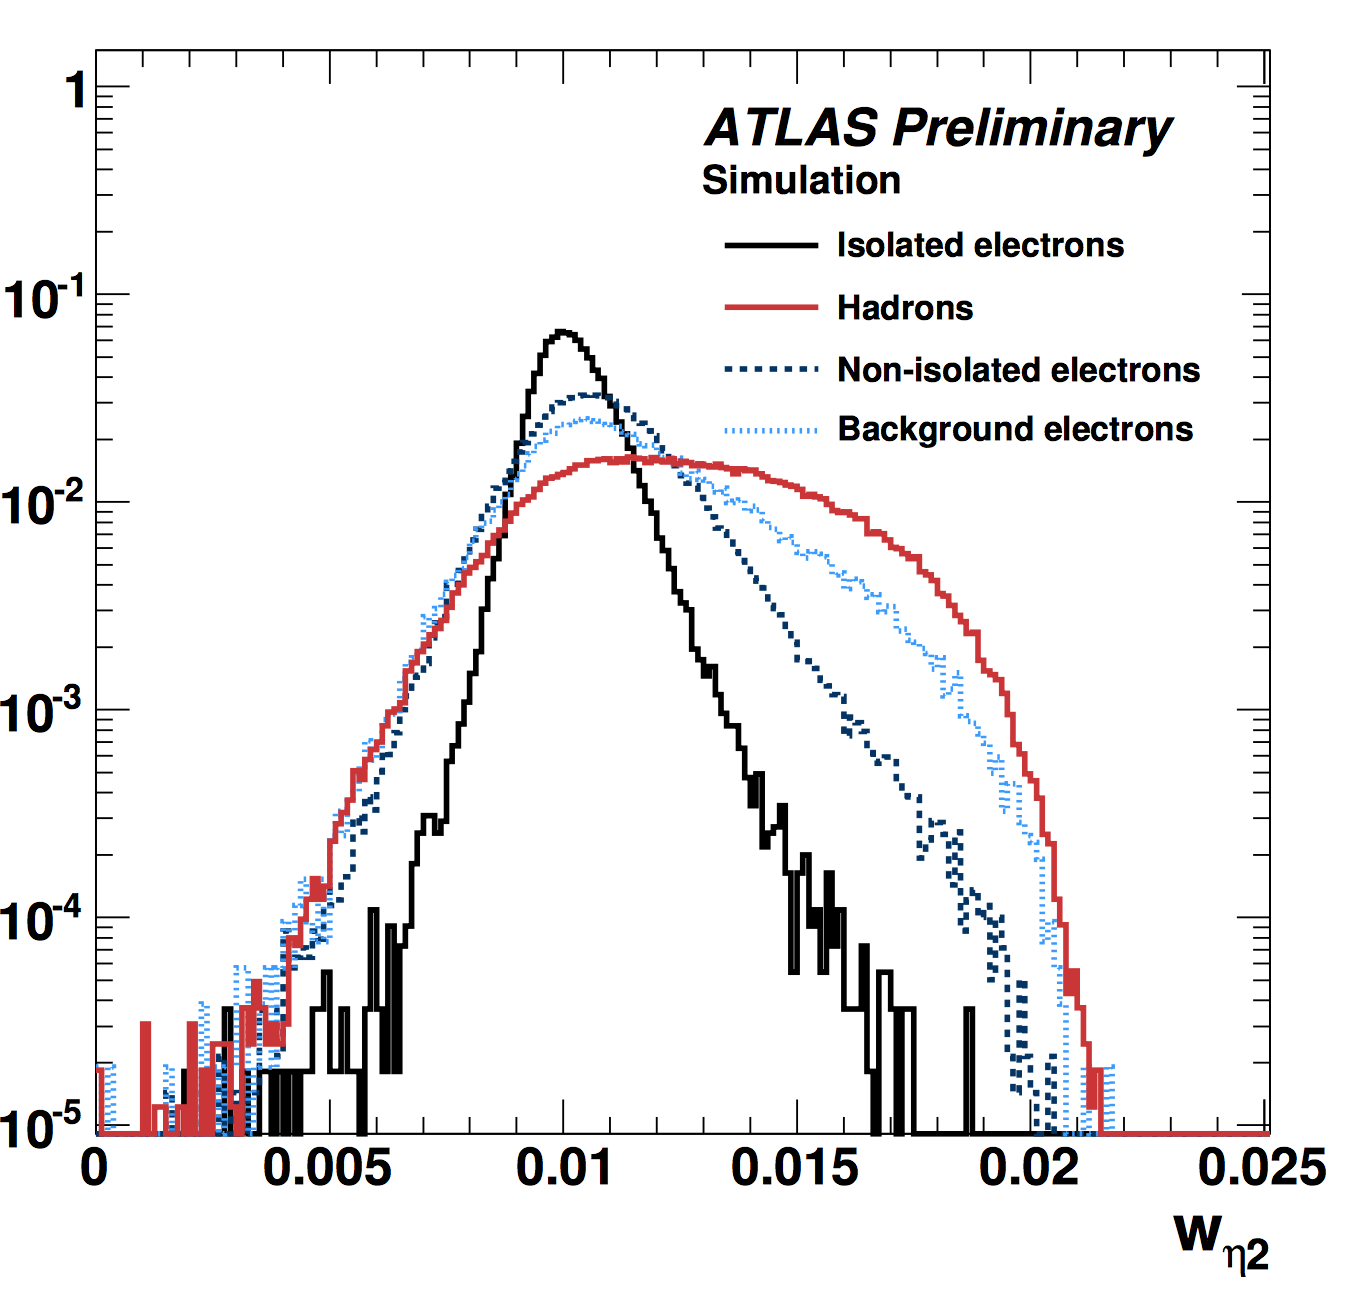
\includegraphics[width=\textwidth,keepaspectratio]{Weta2Simulation.png}
		\caption[ $W_{\eta 2}$]{$W_{\eta 2}$ distribution simulation}
		\label{fig::weta2_simul}
	\end{subfigure}
	\hfill
	\begin{subfigure}[t]{0.39\textwidth} 
		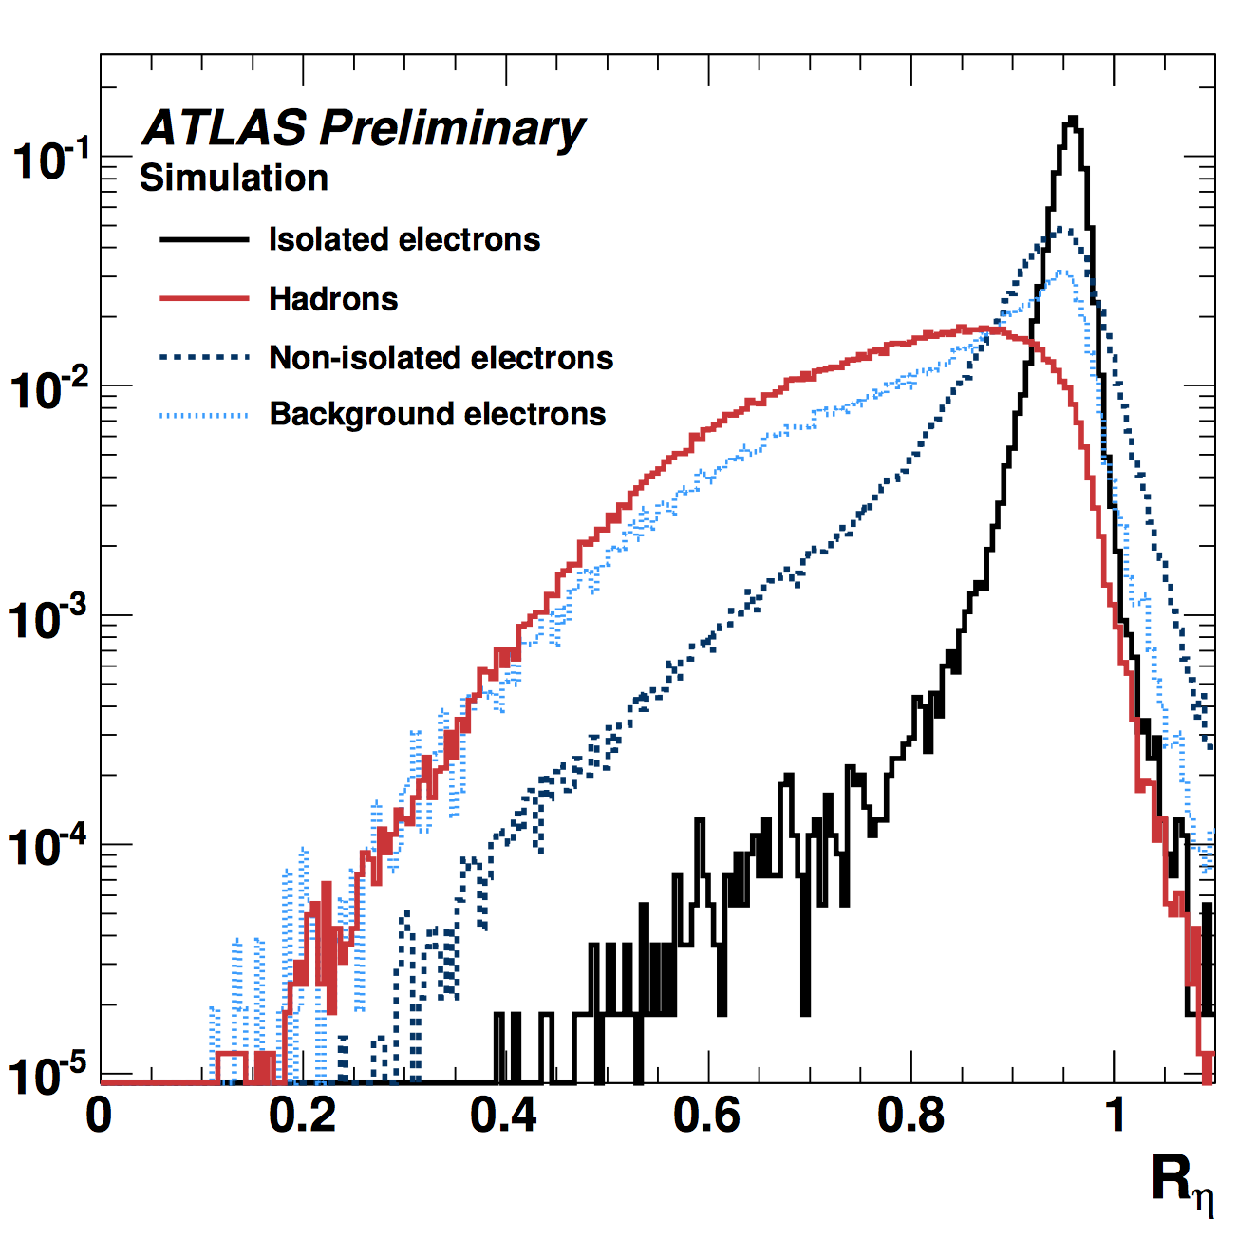
\includegraphics[width=\textwidth,keepaspectratio]{RetaSimulation.pdf}
		\caption[ $R_{\eta}$]{$R_{\eta}$ distribution simulation}
		\label{fig::reta_simul}
	\end{subfigure}
  	\caption{Distribution of $R_{\eta}$ in simulation (GEANT4) for electrons and jets \cite{sshapes_simulation}.}
	\label{fig::sshapes_simul}
\end{figure}

  Figure \ref{fig::sshapes_simul} shows how $R_{\eta}$ distribution is different in jets, signal electrons and background electrons. Background electrons denote non-prompt electrons which are not originated from primary vertex. \\
 
   The shower shapes appear to be extremely sensitive to the detector material modelling. A simplification in the geometry of the EMCal absorber geometry in GEANT4 9.2 (a layered structure of the accordion was represented as a homogeneous material) has lead to visible discrepancies in the shower shapes between the data and MC. This was corrected in GEANT4 9.4 significantly improving the agreement, although not eliminating it completely (see Fig. \ref{fig::sshapes_geant}).  The origin for the remaining discrepancy is not clear.\\
      	\begin{figure}[htbp]
  	\begin{subfigure}[t]{0.4\textwidth}
  		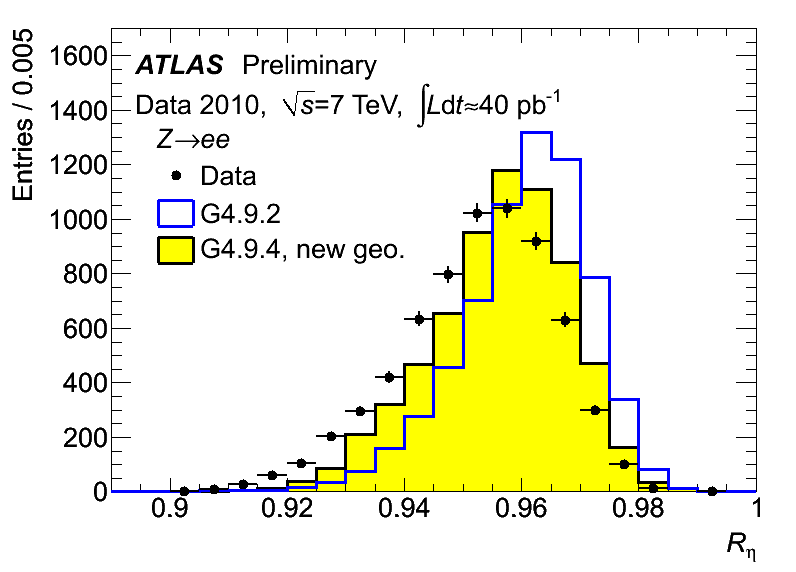
\includegraphics[width=\textwidth,keepaspectratio]{Reta_G}
  		\caption[ $W_{\eta 2}$]{$W_{\eta 2}$}
  		\label{fig::weta2_geant}
  	\end{subfigure}
  	\hfill
  	\begin{subfigure}[t]{0.4\textwidth} 
  		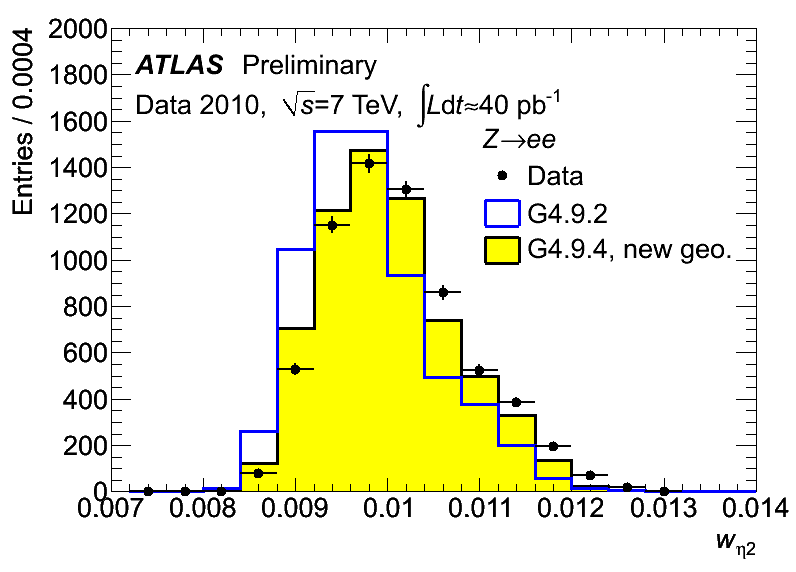
\includegraphics[width=\textwidth,keepaspectratio]{weta2_G}
  		\caption[ $R_{\eta}$]{$R_{\eta}$ }
  		\label{fig::reta_geant}
  	\end{subfigure}
  	\caption{Data/MC Comparison for Calorimeter Shower Shapes of High Et Electrons \cite{geant_corr}.}
  	\label{fig::sshapes_geant}
  \end{figure}
  
  Disagreement in shower shapes between the data and MC leads to discrepancies in particle ID which are later fixed using $\eta-$ and $p_T$-dependent scale factors. Correction of the shower shapes aims to get the scale factors closer to unity, reducing the corresponding systematic uncertainties and improving the precision of the measurements with electrons in the final states.  

  
  \section{ Shower shapes measurement and correction  }
  \subsection{Event selection}
  For this study we have considered electrons from the $Z\rightarrow ee$ decay. A set of recommended single electron triggers was used (HLT\_e26\_lhtight\_nod0\_ivarloose,\\ HLT\_e60\_lhmedium\_nod0,\\
   HLT\_e140\_lhloose\_nod0,HLT\_e300\_etcut). Each event was required to have 2 electrons at least one of which has $p_T>25$ GeV.  In order to suppress the background both electrons had to pass gradient isolation. Z invariant mass cut was applied with a window of $80-120$GeV. To avoid identification bias from triggering the tag and probe approach was used with only probe electrons taken into consideration \cite{RecoID2011}. The electron cluster in the second calorimeter layer was required to contain information from 77 calorimeter cells. No pile-up reweighting has been applied. Datasets of 264786295 events in data (2017 proton-proton collisions) and 79340000 events in MC (Powheg+Pythia8) were used. 
  \subsection{Data/MC discrepancies}
  Our consideration begins with the energy deposit of an electron in the second layer of the calorimeter. A window of 7 cells in $\eta$ and 11 cells in $\phi$ is centred around the cell with the highest energy.

  Shower shapes were considered in 14 $\eta$ bins in the range between $|\eta| = (0,2.4)$ in order to investigate how the discrepancy depends on $\eta$. 
    	\begin{figure}[htbp]
  	\begin{subfigure}[t]{0.5\textwidth}
  		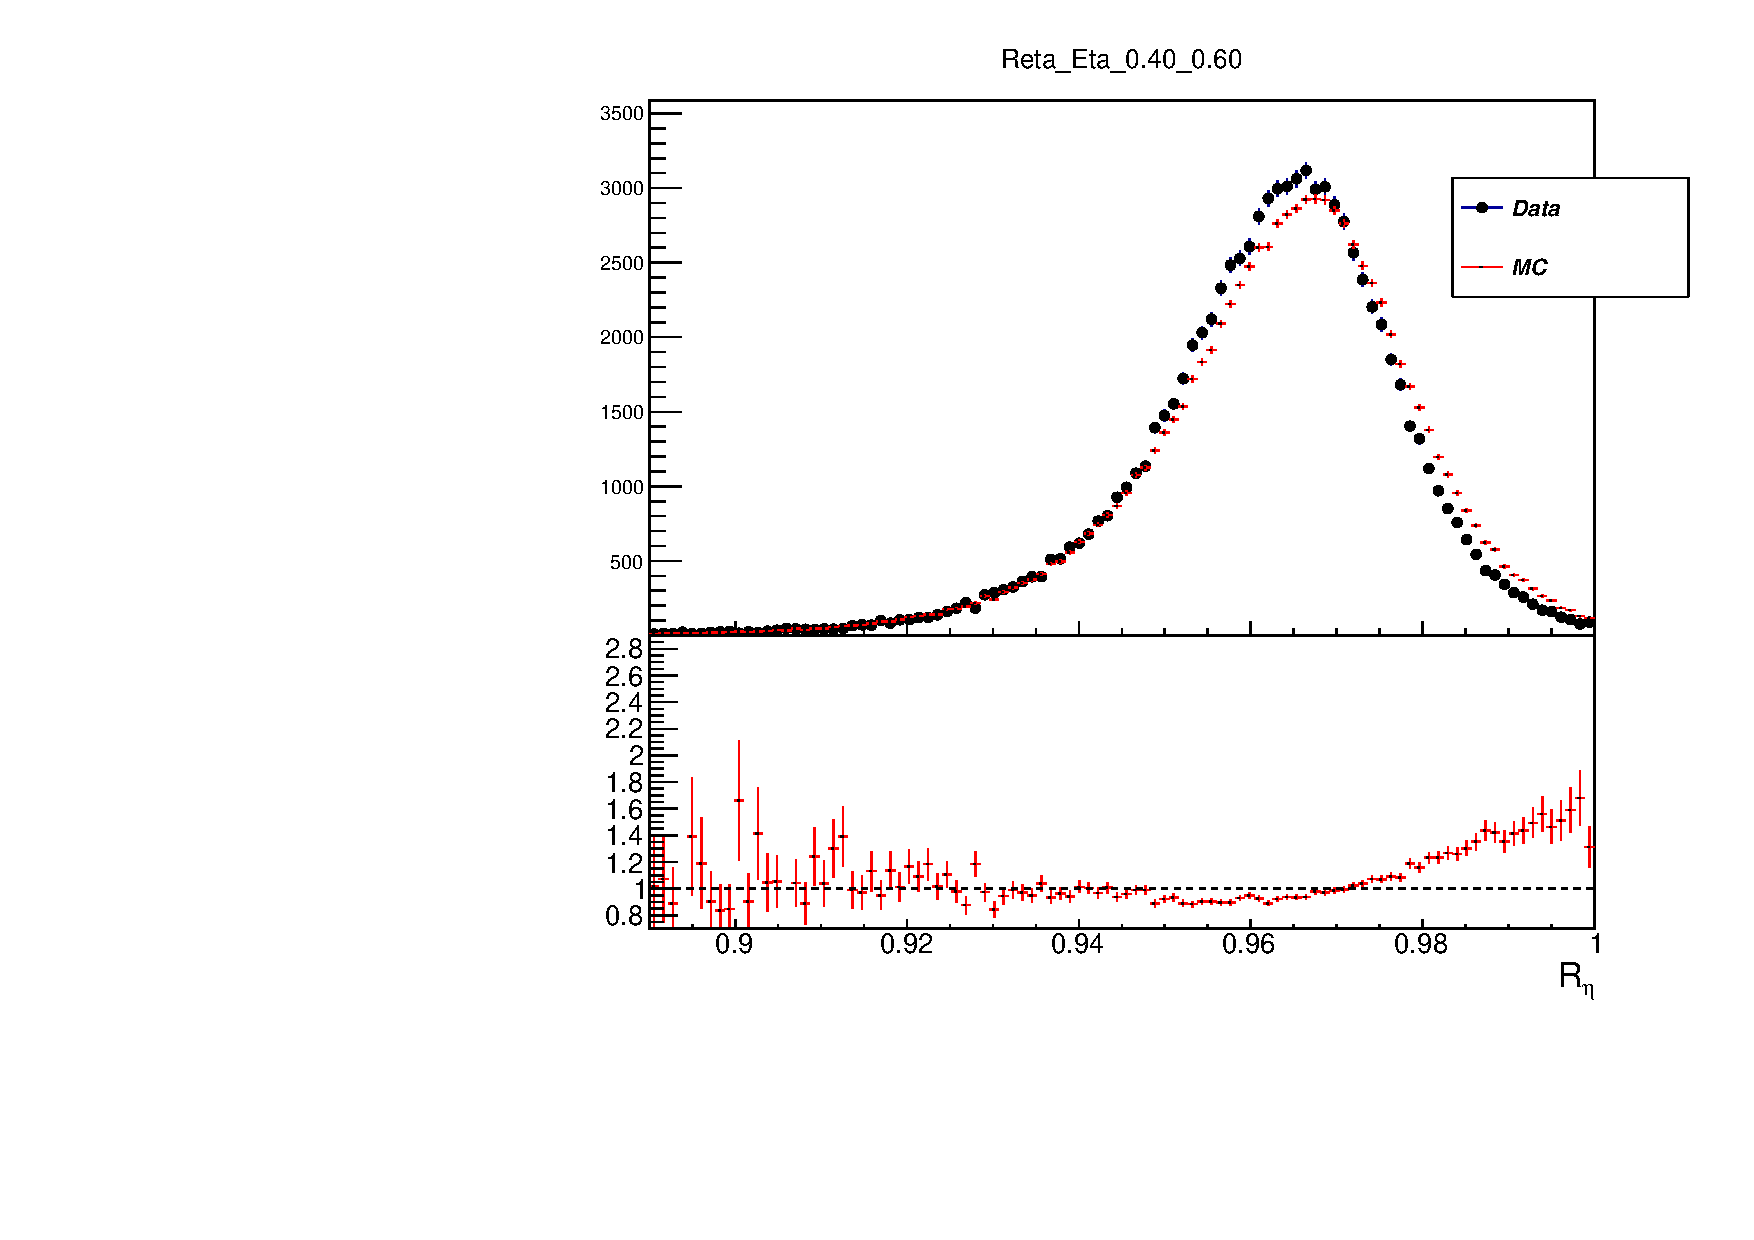
\includegraphics[width=\textwidth,keepaspectratio]{Reta2_Eta_4_6.pdf}
  		\caption{$R_{\eta}$ in $|\eta| = (0.4,0.6)$ }
  		\label{fig::reta_norew_04}
  	\end{subfigure}
  	\hfill
  	\begin{subfigure}[t]{0.5\textwidth} 
  		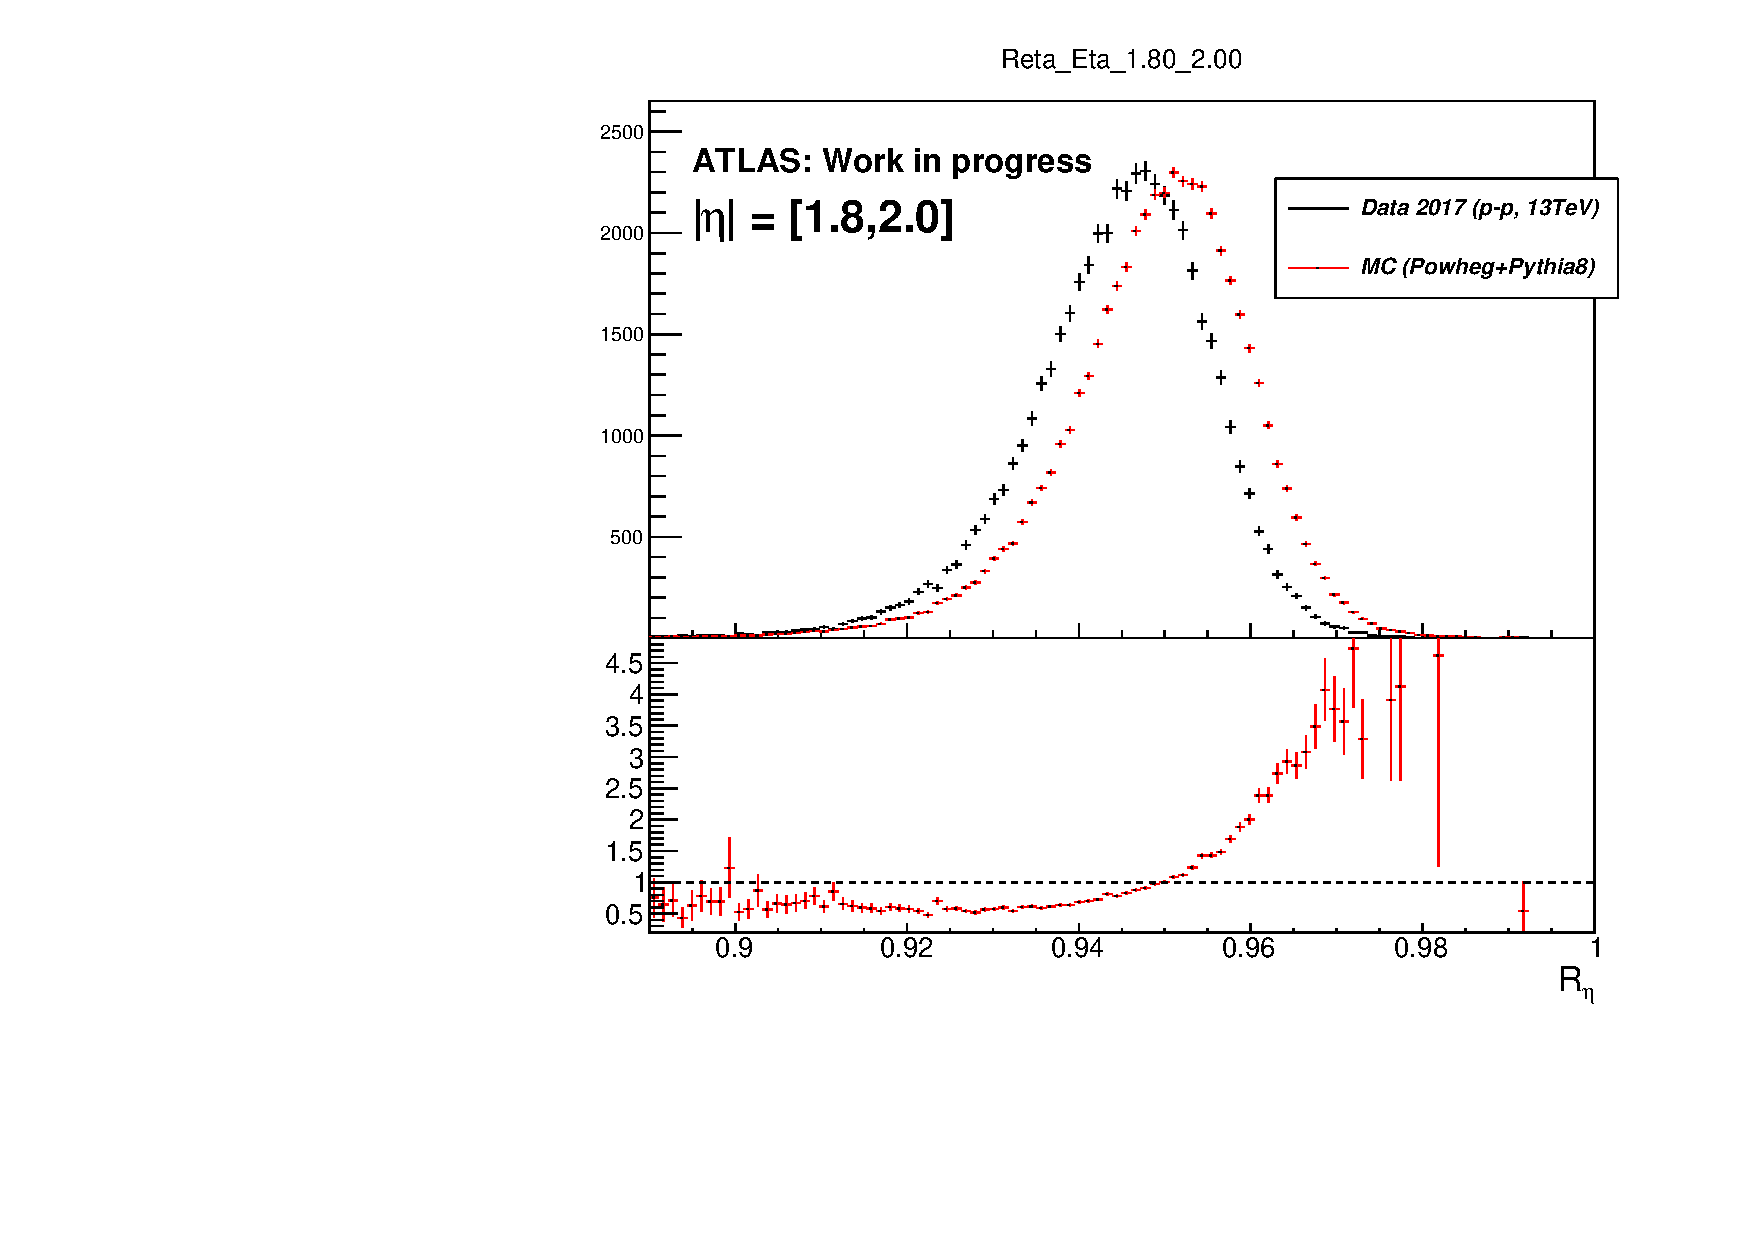
\includegraphics[width=\textwidth,keepaspectratio]{Reta2_Eta_18_20.pdf}
  		\caption{$R_{\eta}$ in $|\eta| = (1.8,2.0)$ }
  		\label{fig::reta_norew_18}
  	\end{subfigure}
  	\caption{$R_{\eta}$ in the barel and in the end-cap, Data vs MC}
  	\label{fig::reta_norew}
  \end{figure}

    \begin{figure}[htbp]
	\begin{subfigure}[t]{0.5\textwidth}
		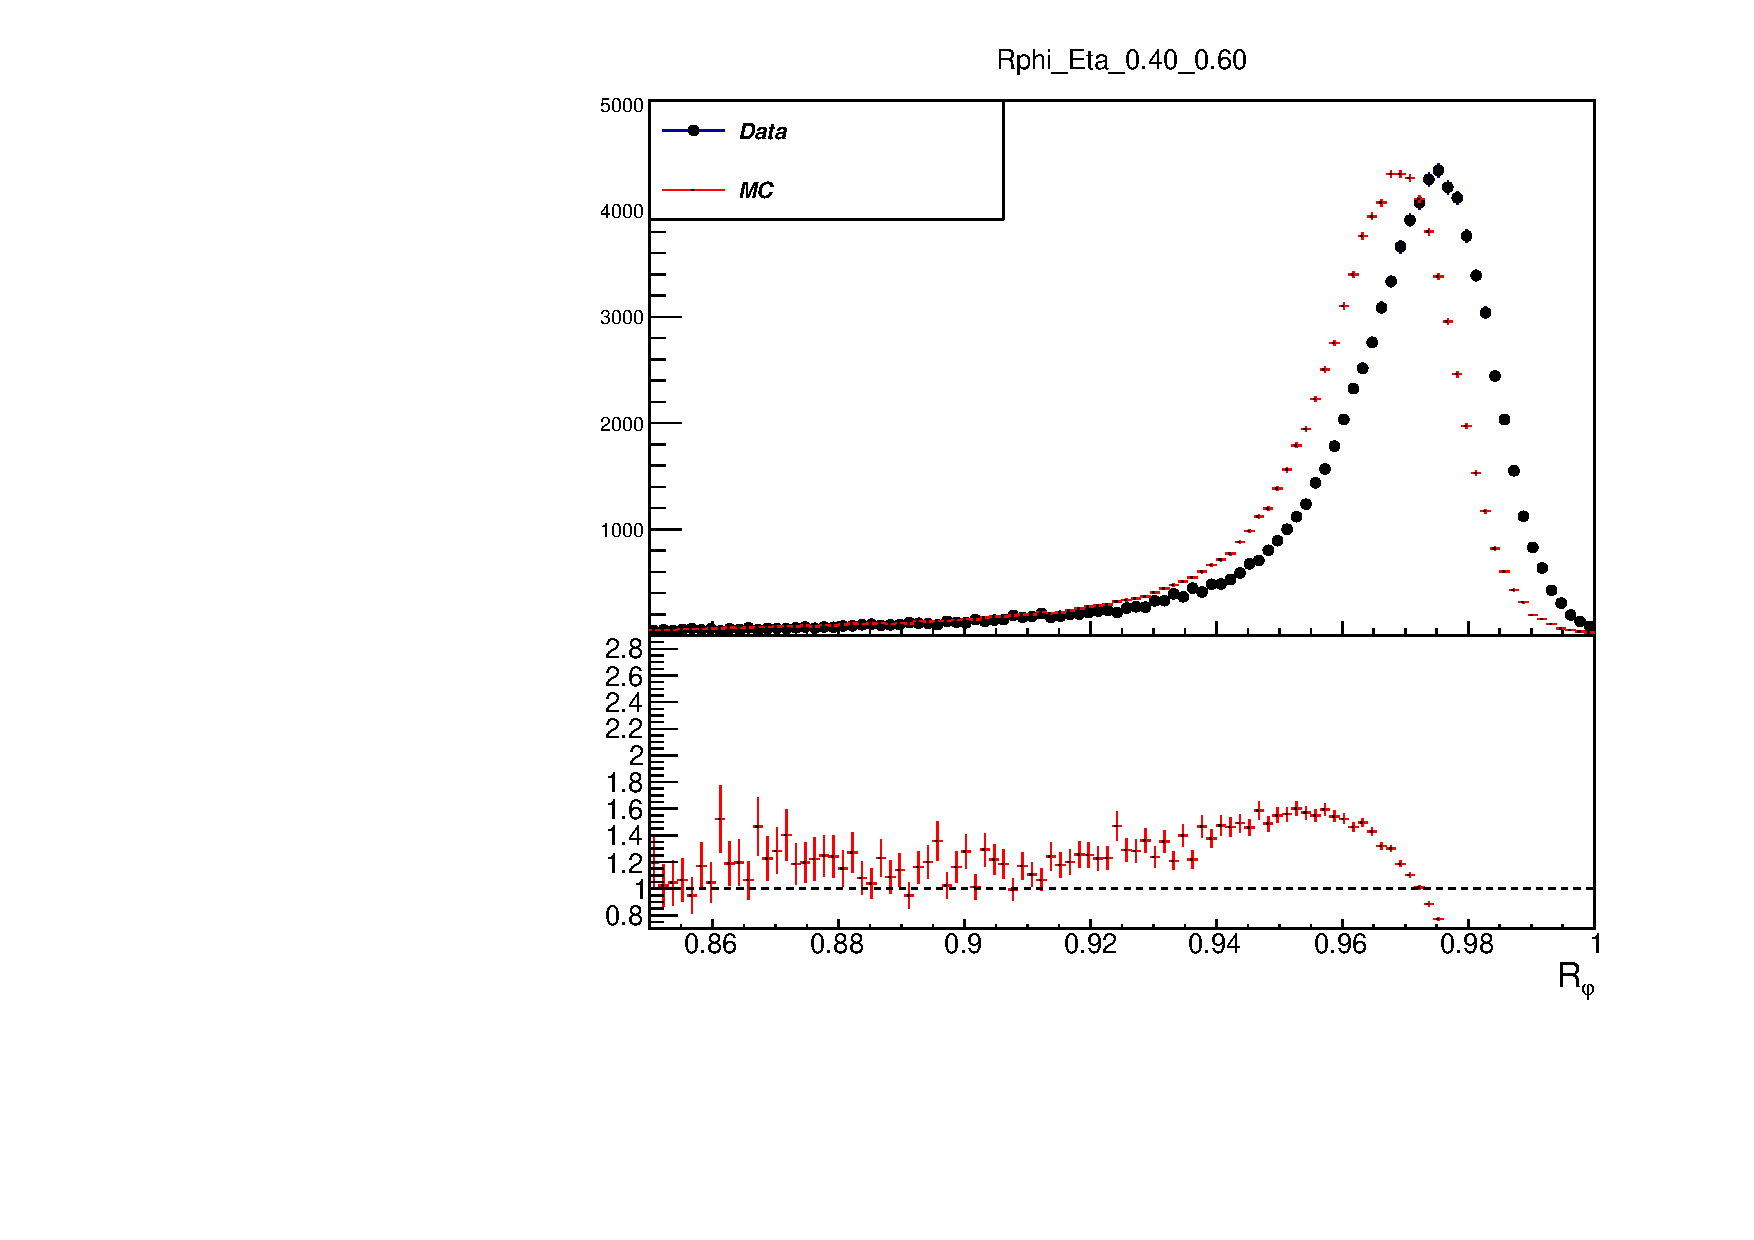
\includegraphics[width=\textwidth,keepaspectratio]{Rphi2_Eta_4_6.pdf}
		\caption{$R_{\phi}$ in $|\eta| = (0.4,0.6)$ }
		\label{fig::rphi_norew_04}
	\end{subfigure}
	\hfill
	\begin{subfigure}[t]{0.5\textwidth} 
		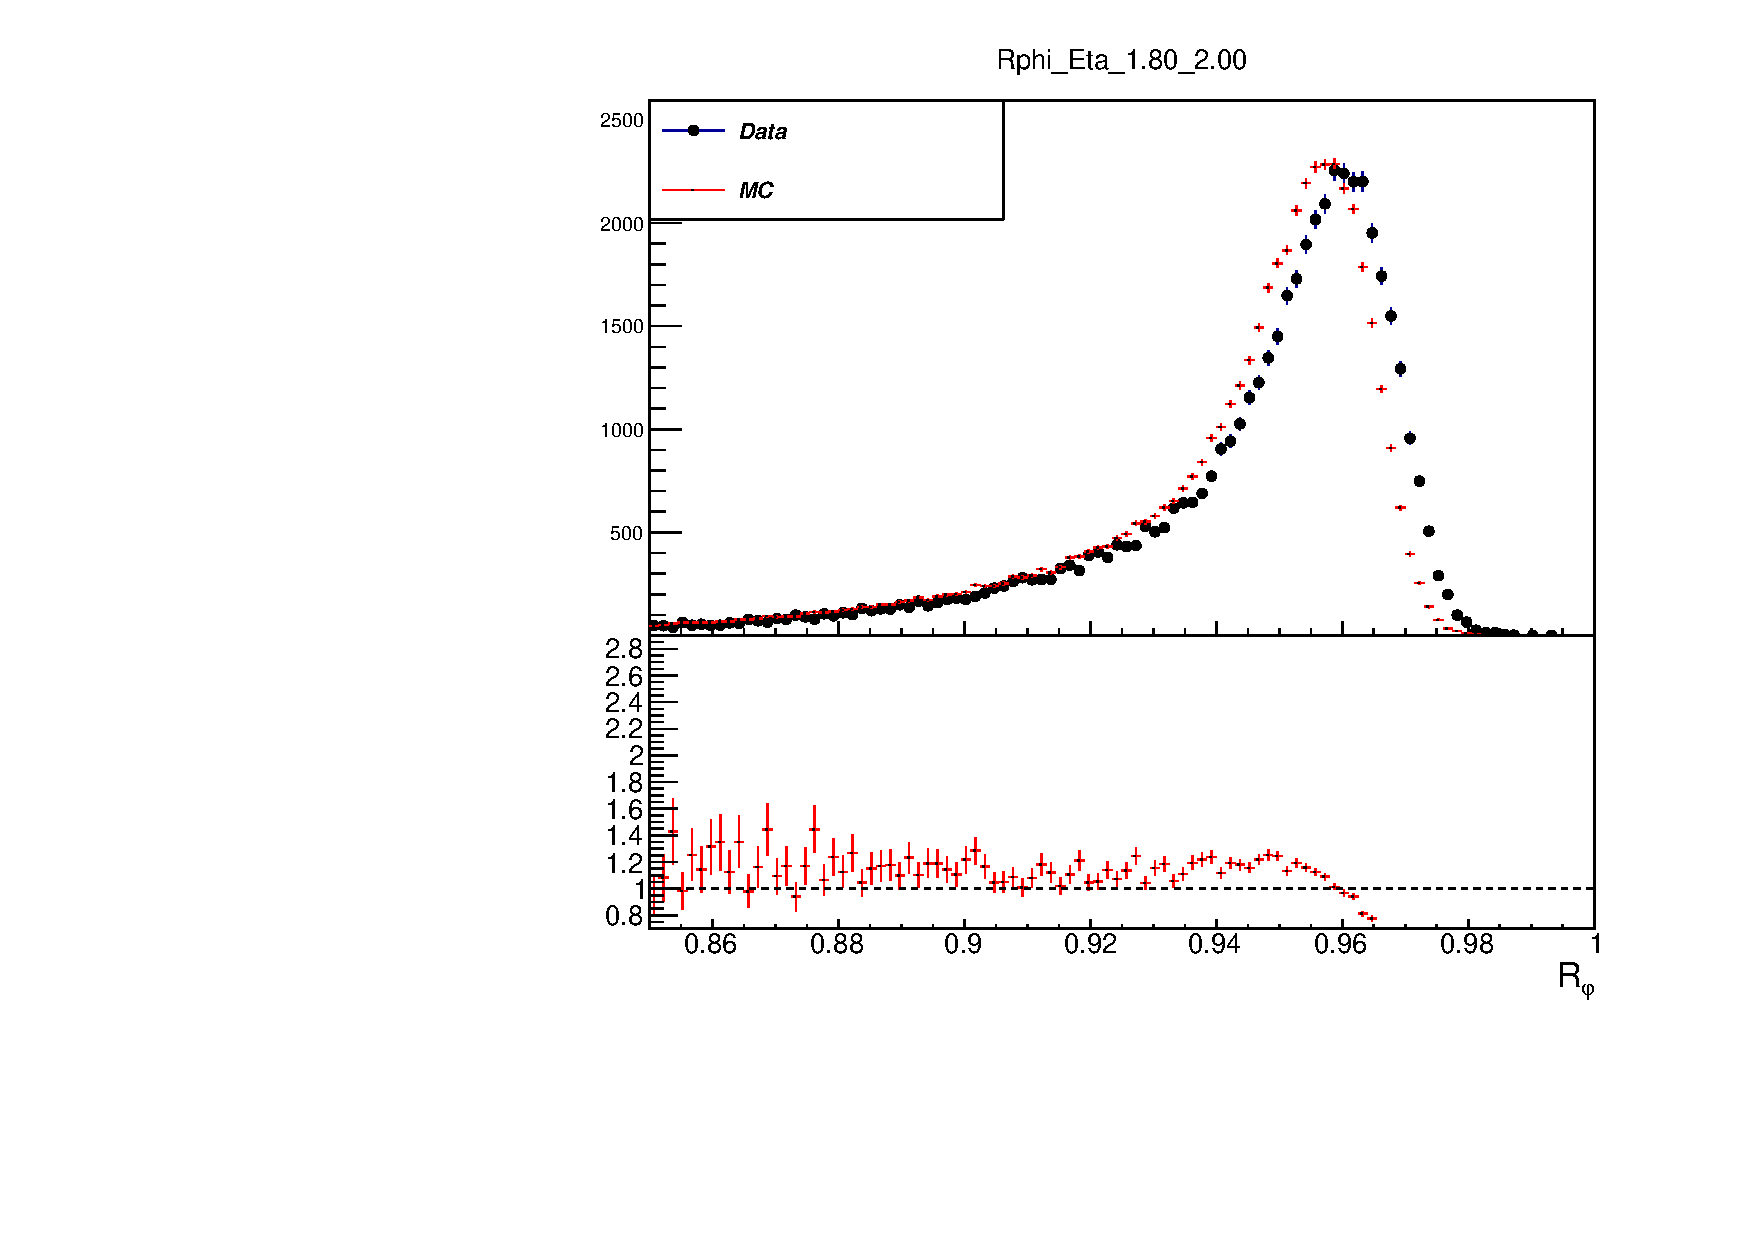
\includegraphics[width=\textwidth,keepaspectratio]{Rphi2_Eta_18_20.pdf}
		\caption{$R_{\phi}$ in $|\eta| = (1.8,2.0)$ }
		\label{fig::rphi_norew_18}
	\end{subfigure}
	\caption{$R_{\phi}$ in the barel and in the end-cap, Data vs MC}
	\label{fig::rphi_norew}
\end{figure}
  
    \begin{figure}[htbp]
	\begin{subfigure}[t]{0.5\textwidth}
		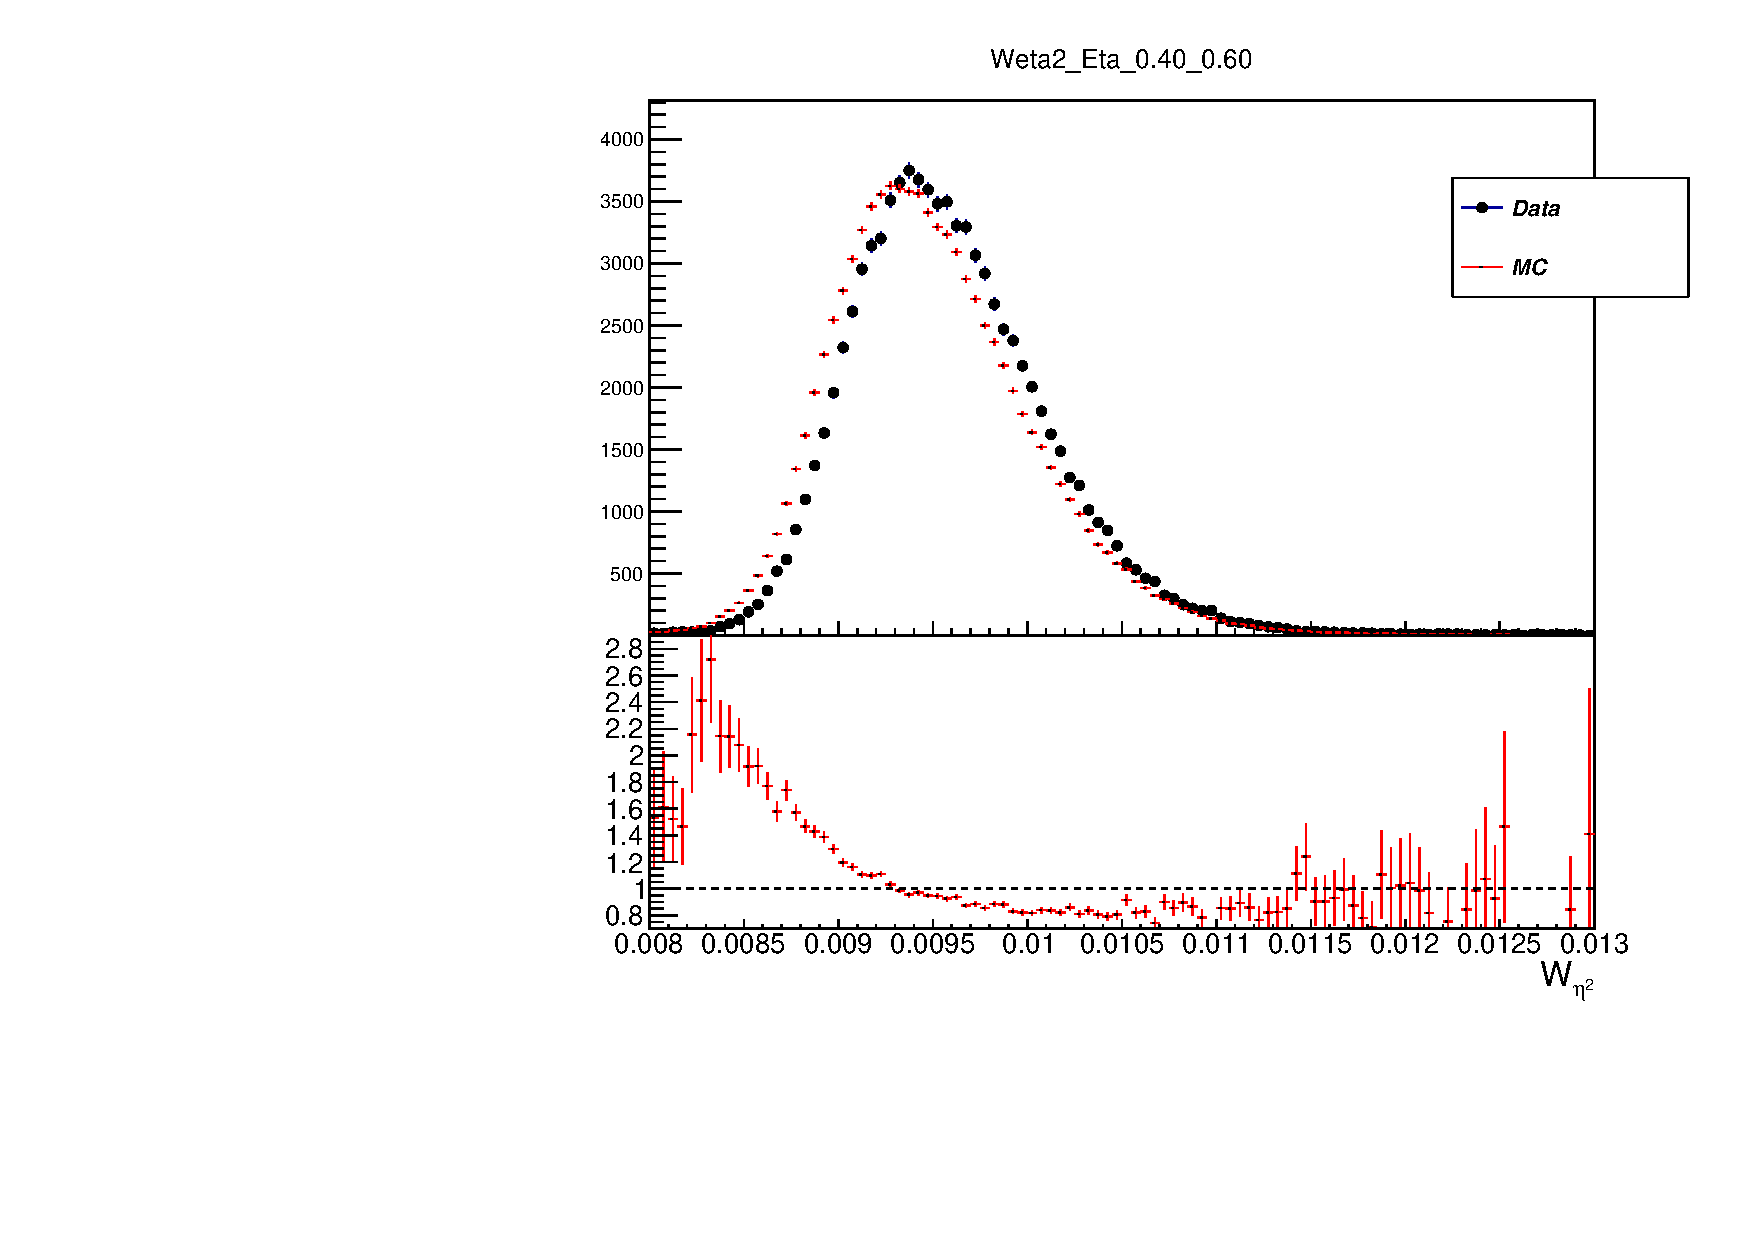
\includegraphics[width=\textwidth,keepaspectratio]{weta22_Eta_4_6.pdf}
		\caption{$W_{\eta}^2$ in $|\eta| = (0.4,0.6)$ }
		\label{fig::weta2_norew_04}
	\end{subfigure}
	\hfill
	\begin{subfigure}[t]{0.5\textwidth} 
		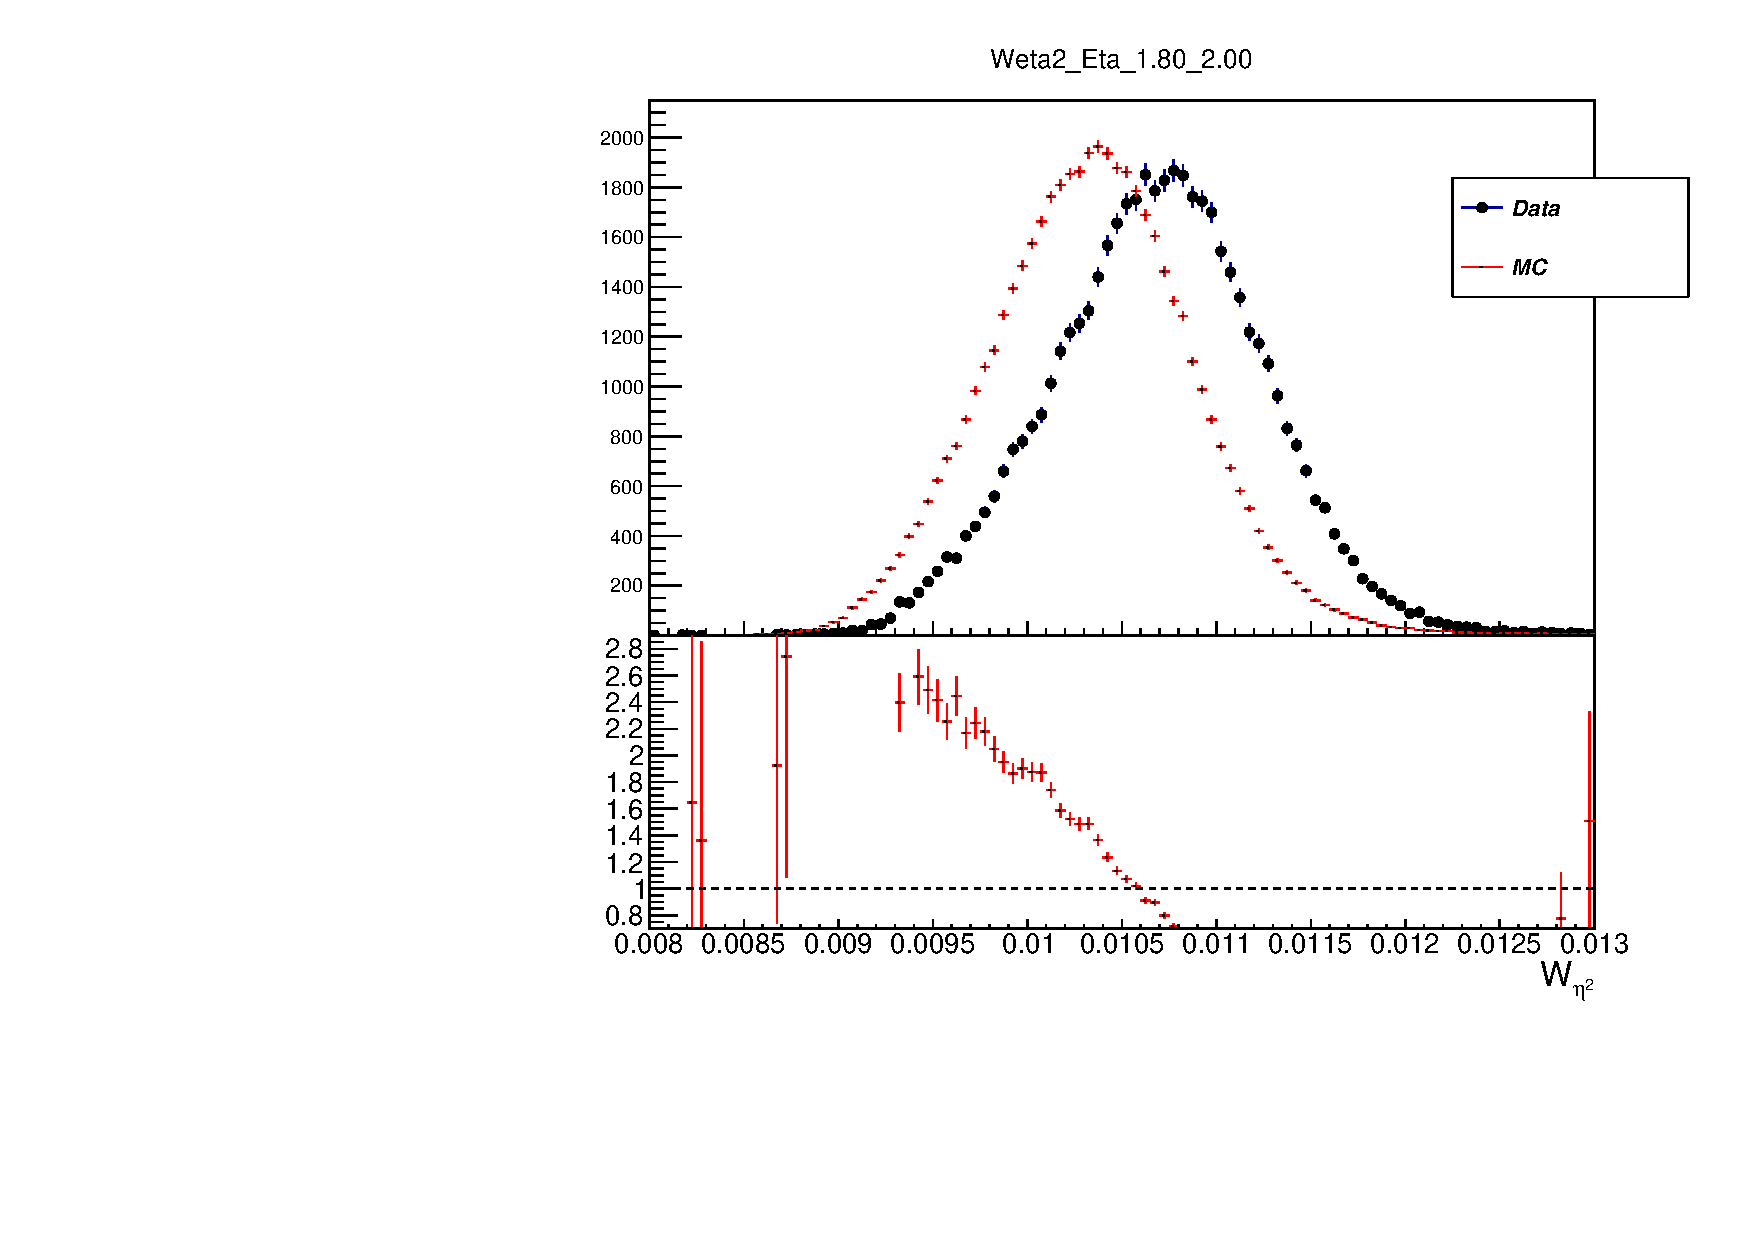
\includegraphics[width=\textwidth,keepaspectratio]{weta22_Eta_18_20.pdf}
		\caption{$W_{\eta}^2$ in $|\eta| = (1.8,2.0)$ }
		\label{fig::weta2_norew_18}
	\end{subfigure}
	\caption{$W_{\eta}^2$ in the barel and in the end-cap, Data vs MC}
	\label{fig::weta2_norew}
\end{figure}



  The $\eta$-dependent shower shapes in data are wider than the MC and show a larger discrepancy in the endcap ($|\eta| = (1.52,2.4)$). For $\phi$ dimension the situation is the opposite: MC is wider than the data and the barrel ($|\eta| = (0,1.52)$) shows larger discrepancy. Figures \ref{fig::reta_norew}, \ref{fig::rphi_norew}, \ref{fig::weta2_norew} contain examples of shower shapes in different eta bins. 
  \subsection{The correction procedure}
  \subsubsection{The correction matrix}
  The correction procedure is based on the redistribution of energy between the cluster cells in MC so that the distribution becomes consistent with the data. For every $\eta$ bin a correction matrix is derived in the following way:
  \begin{equation}
  \nonumber
  \large {M_{i}^{Correction} = \frac{E_{i}^{Data}}{\Sigma E^{Data}} - \frac{E_{i}^{MC}}{\Sigma E^{MC}}}
  \end{equation}
  $\Sigma_i M_i^{Correction} = 0$, $i = 1..77$.\\
  $E_i^{Data}$, $E_i^{MC}$ - matrix elements of the averaged energy profiles. 
  The correction is then applied to the electron cluster cells on event-by-event basis:
  \begin{equation}
  \nonumber
  \large {E_{i}^{Reweighted} = {E_{i}^{Non-reweighted}(1+M_{i}^{Correction}).}}
  \end{equation}
  This redistributes the energy among the cells keeping the total energy exactly the same.
  \subsubsection{Bremsstrahlung tails}
  The magnetic field directed along the $\phi$ dimension leads to a significant asymmetry in the energy deposits for electrons and positrons (Fig. \ref{fig::chargeAsym}). 
  
  
      \begin{figure}[htbp]
  	\begin{subfigure}[t]{0.5\textwidth}
  		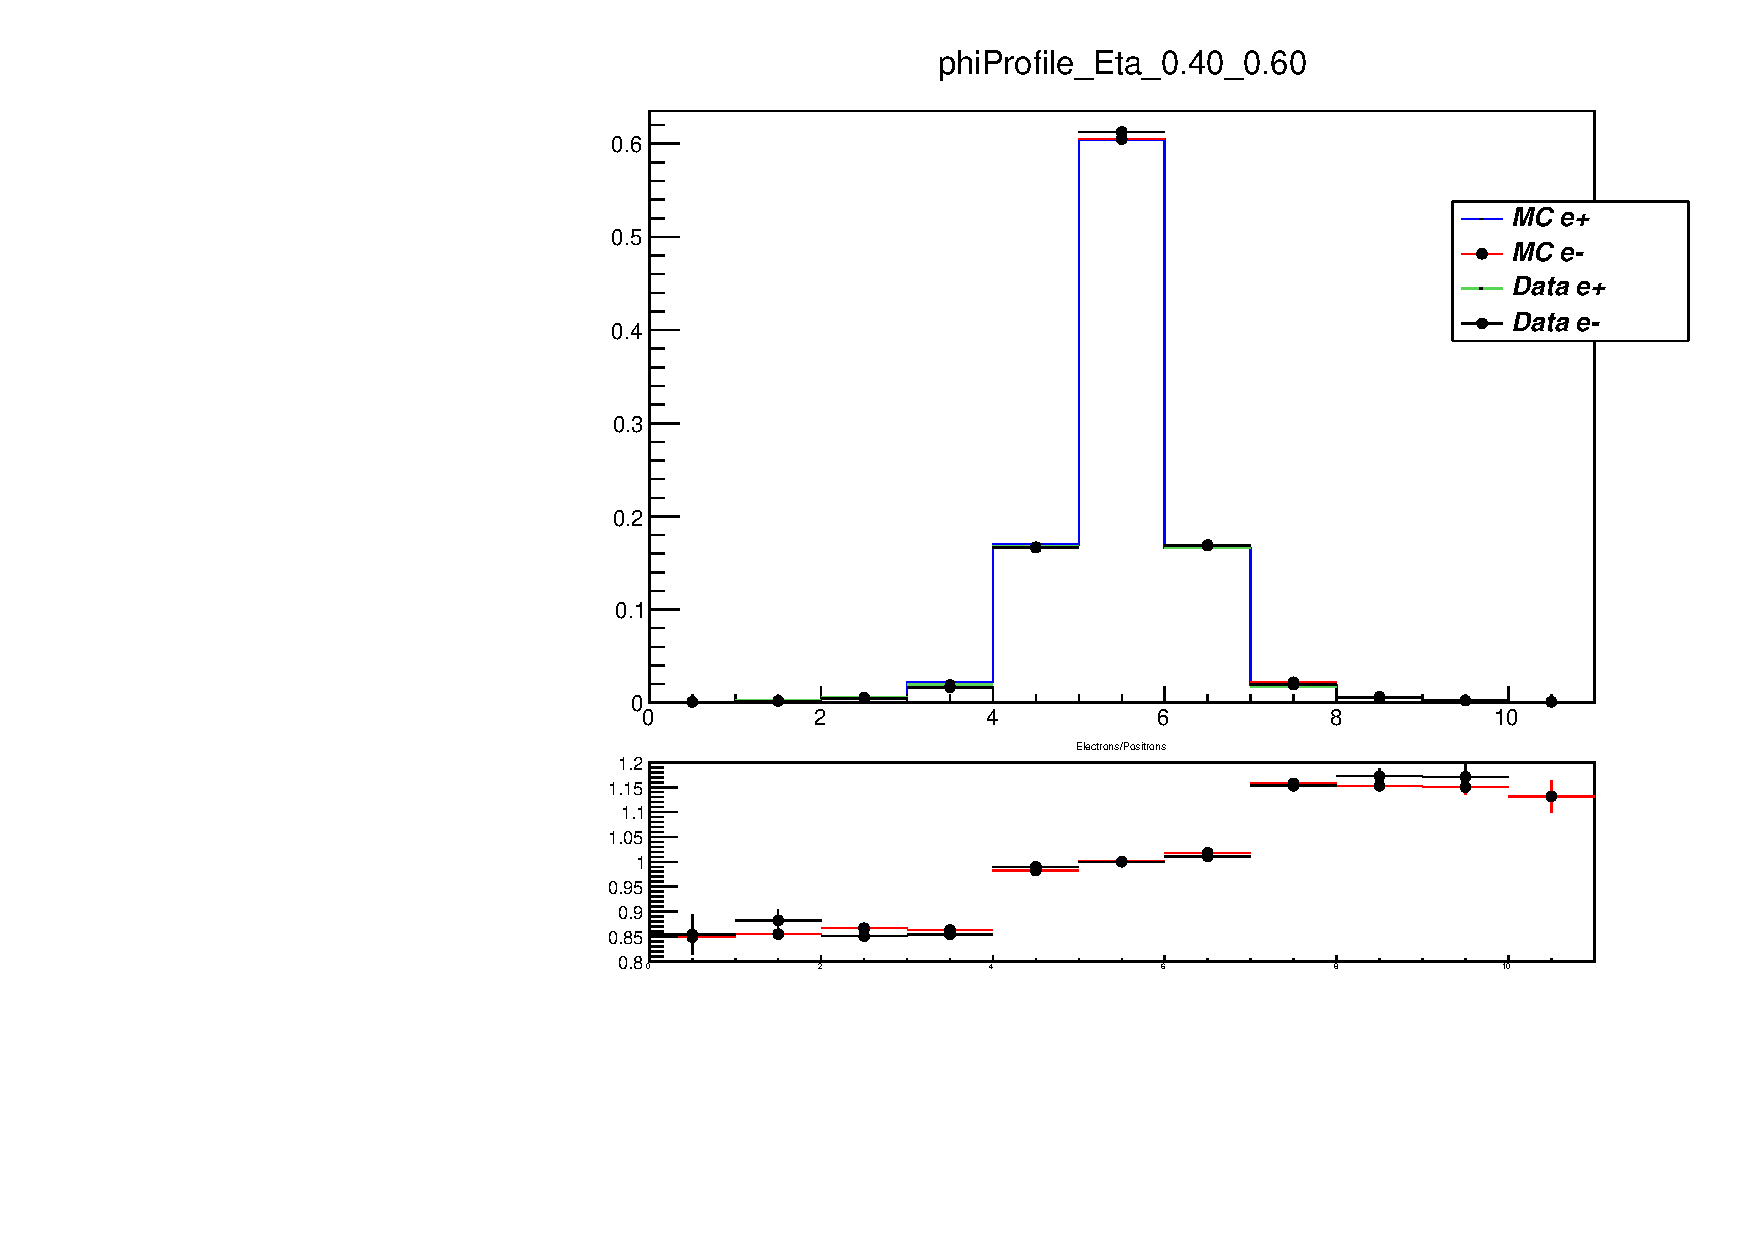
\includegraphics[width=\textwidth,keepaspectratio]{phiProfileDataMC_Eta_4_6.pdf}
  		\caption{$R_{\phi}$ in $|\eta| = (0.4,0.6)$ }
  		\label{fig::phi_profile_04}
  	\end{subfigure}
  	\hfill
  	\begin{subfigure}[t]{0.5\textwidth} 
  		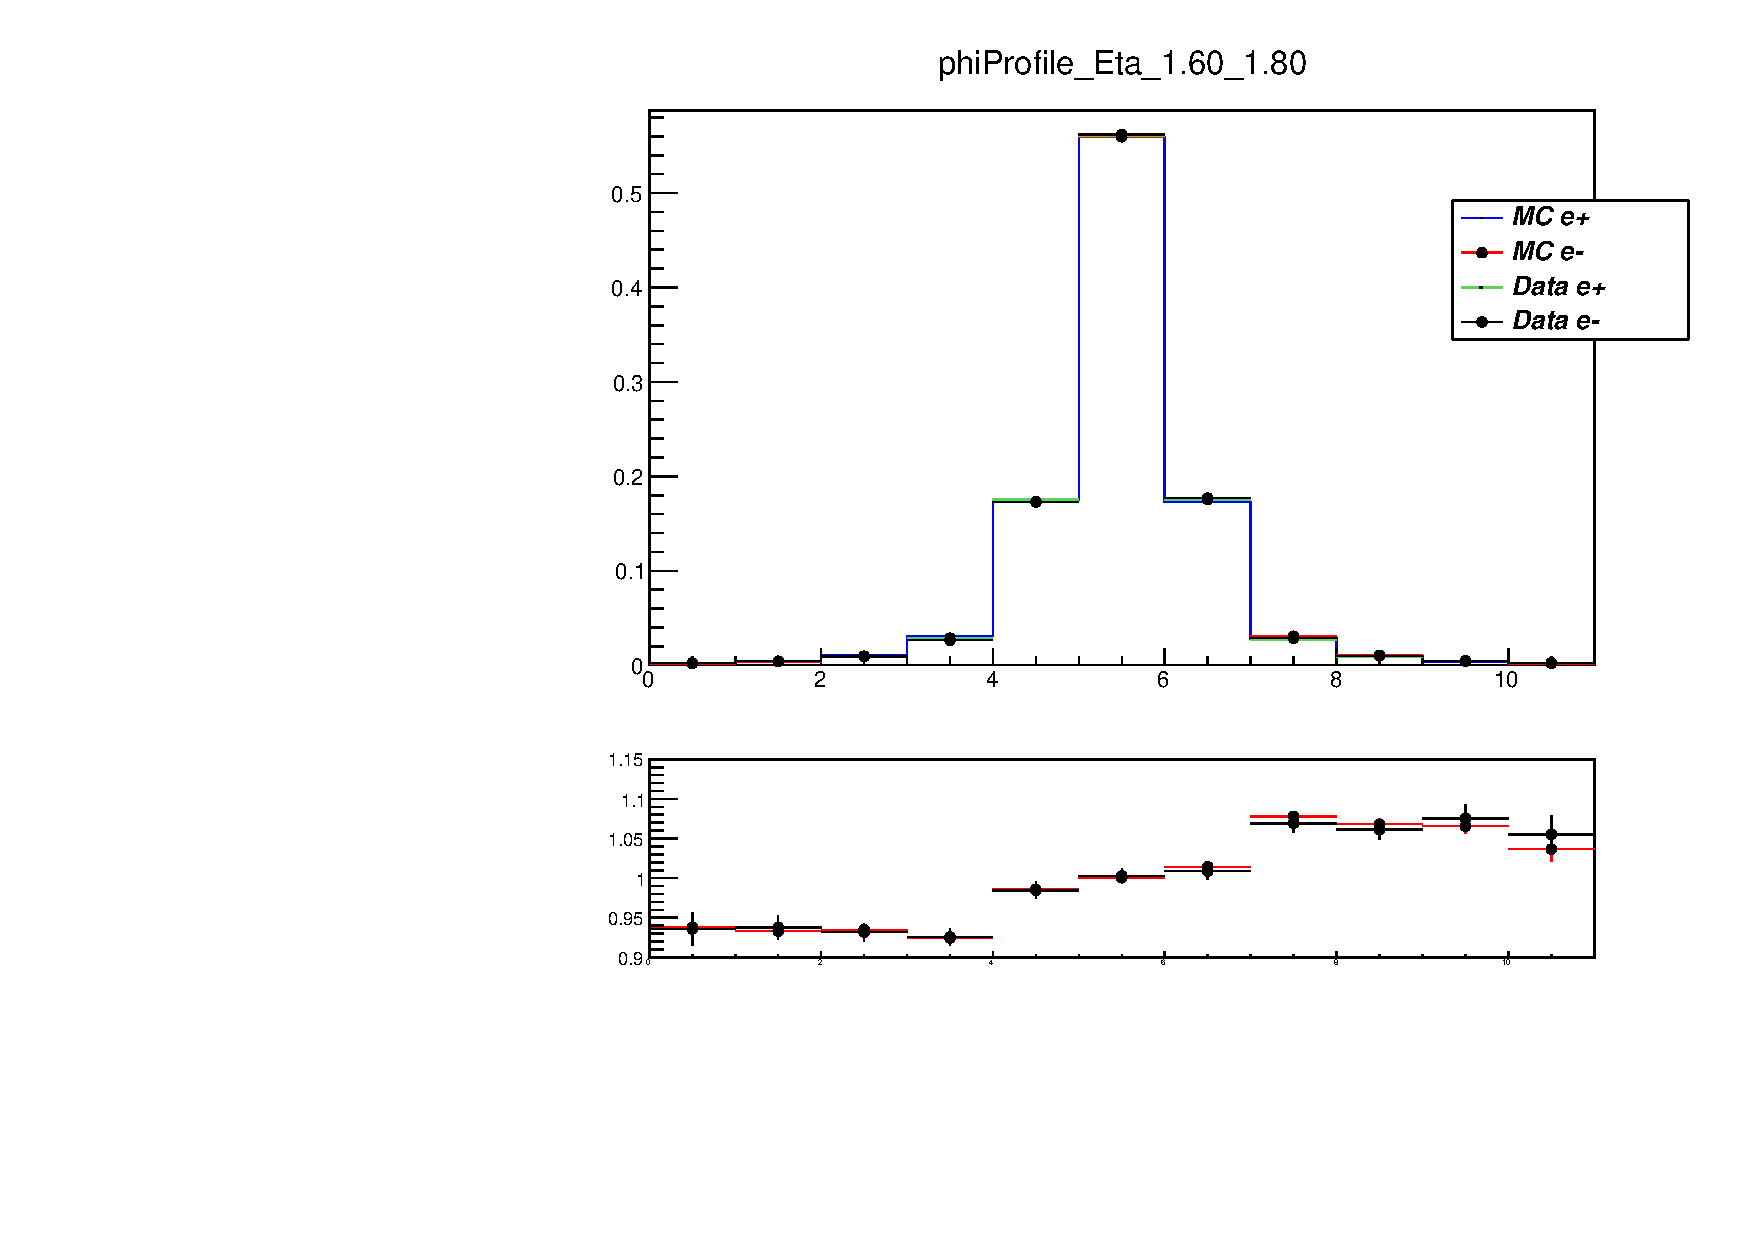
\includegraphics[width=\textwidth,keepaspectratio]{phiProfileDataMC_Eta_16_18.pdf}
  		\caption{$R_{\phi}$ in $|\eta| = (1.8,2.0)$ }
  		\label{fig::phi_profile_18}
  	\end{subfigure}
  	\caption{$R_{\phi}$ in the barrel and in the end-cap for $e^+$ and $e^-$ in Data and MC. The ratio panel shows $e^+/e^-$ energy deposits in Data (black) and MC (red).}
  	\label{fig::chargeAsym}
  \end{figure}

  
  Considering the fact that the reweighting is intended to correct for the data/MC discrepancies themselves and not for the bremsstrahlung effect it makes sense to develop the bremsstrahlung-free correction function based on $e^+$ and $e^-$ correction matrices. The principle is schematically explained on figure \ref{bstails}.\\
  \begin{figure}[htbp]
  	\begin{center}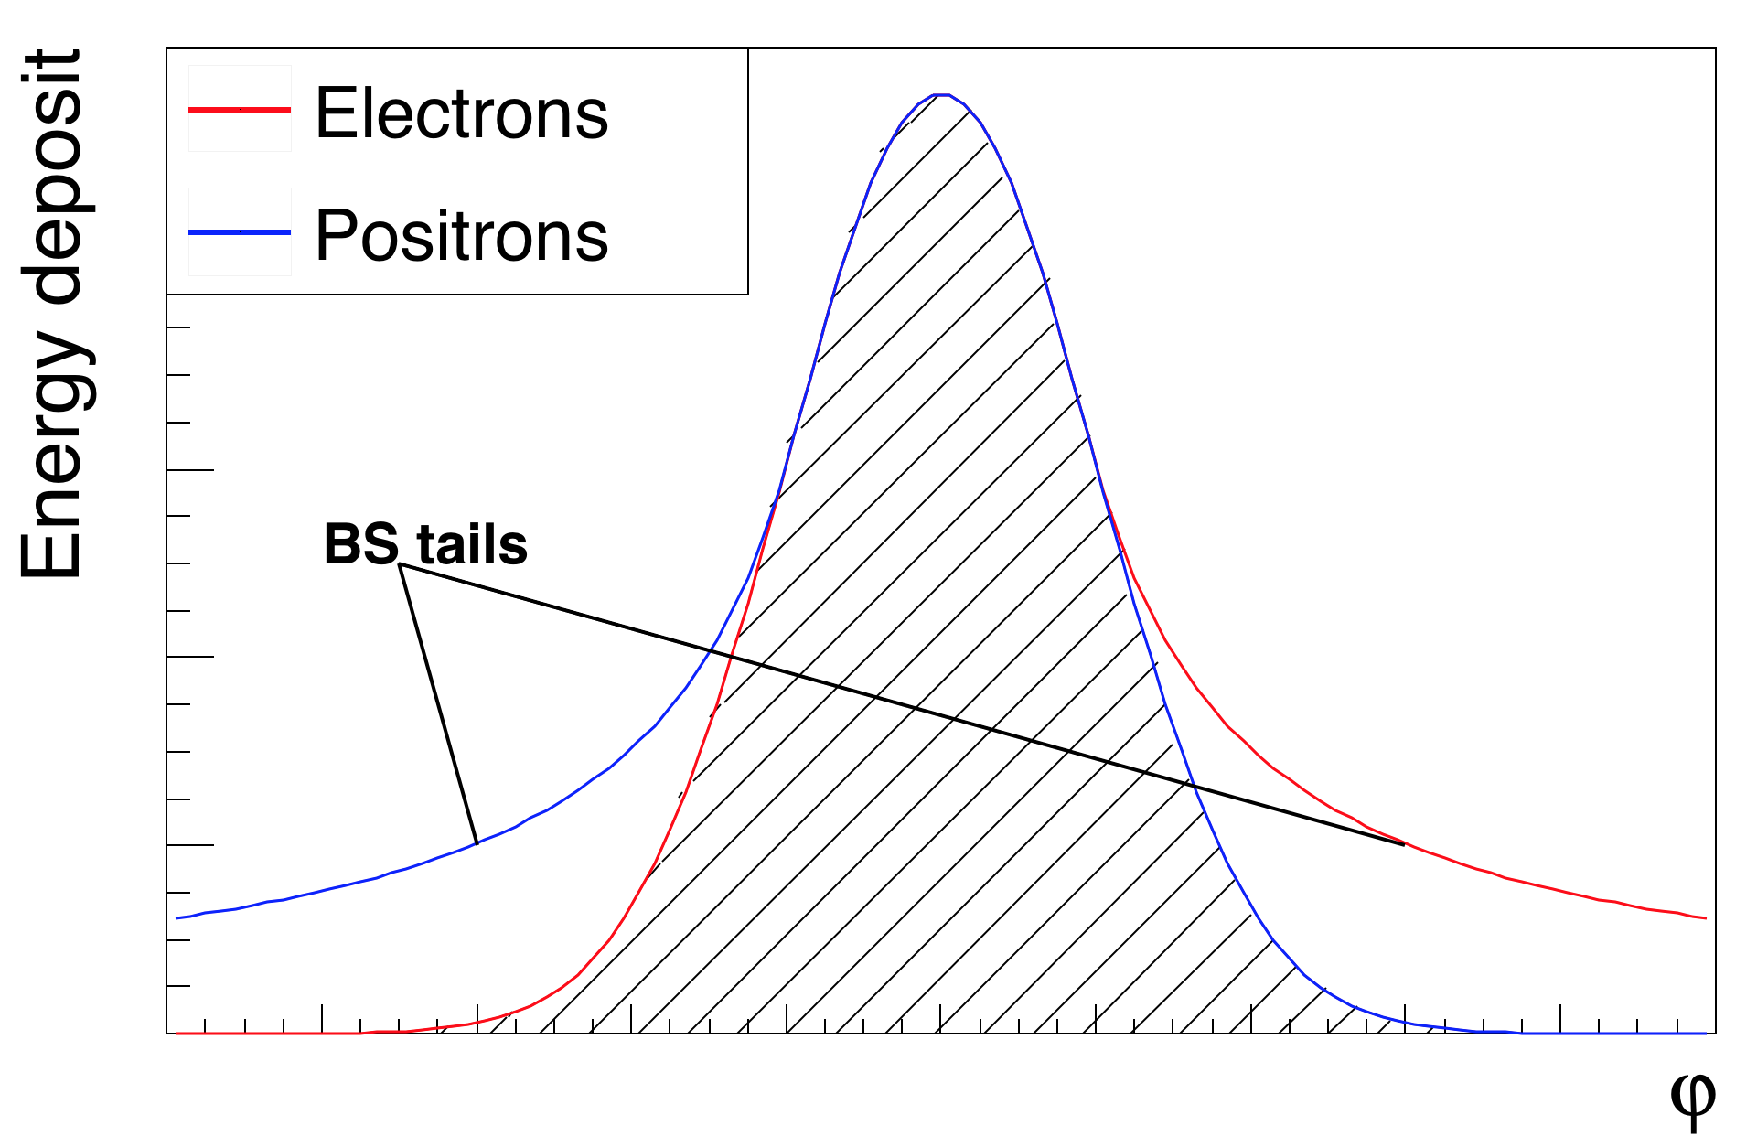
\includegraphics[%
  		width=7cm,
  		keepaspectratio]{bs_tails.pdf}\end{center}
  	\caption{Schematic energy profile in $\phi$ dimension. Bremsstrahlung tails subtraction based on $e^+$ and $e^-$ energy profiles.}
  	\label{bstails}
  \end{figure}
  Good agreement of data and MC description of $e^+$ and $e^-$ asymmetry gives a hint that the material mismodelling cannot be the main source of the data/MC disagreement.\\
  
  \section{Results}
  Figures \ref{fig::reta}, \ref{fig::rphi_rew}, \ref{fig::weta2_rew} show the effect of the correction. The shower shapes in MC become very close to the data, correcting a significant discrepancy. 
  
  Figures \ref{fig::integrated} contain shower shapes vs $p_T$ integrated over $\eta$. They demonstrate that the correction does not depend on the $p_T$ which allows to expect the decreased systematic uncertainties for $p_T$ regions distant from $40-50$GeV.\\
  Finally, figure \ref{SF} shows the effect of the correction on electron ID efficiency. We can see a visible improvement, notably in the endcap region.
  Nevertheless the barrel region shows little improvement. It can be explained by the fact that electron ID MVA relies on many variables while only a number of them were corrected during current study.\\
  The proposed method is getting integrated into ATLAS Athena framework as an option and is planned to be used as a baseline for Run 3. 
  
  	\begin{figure}[htbp]
  	\begin{subfigure}[t]{0.5\textwidth}
  		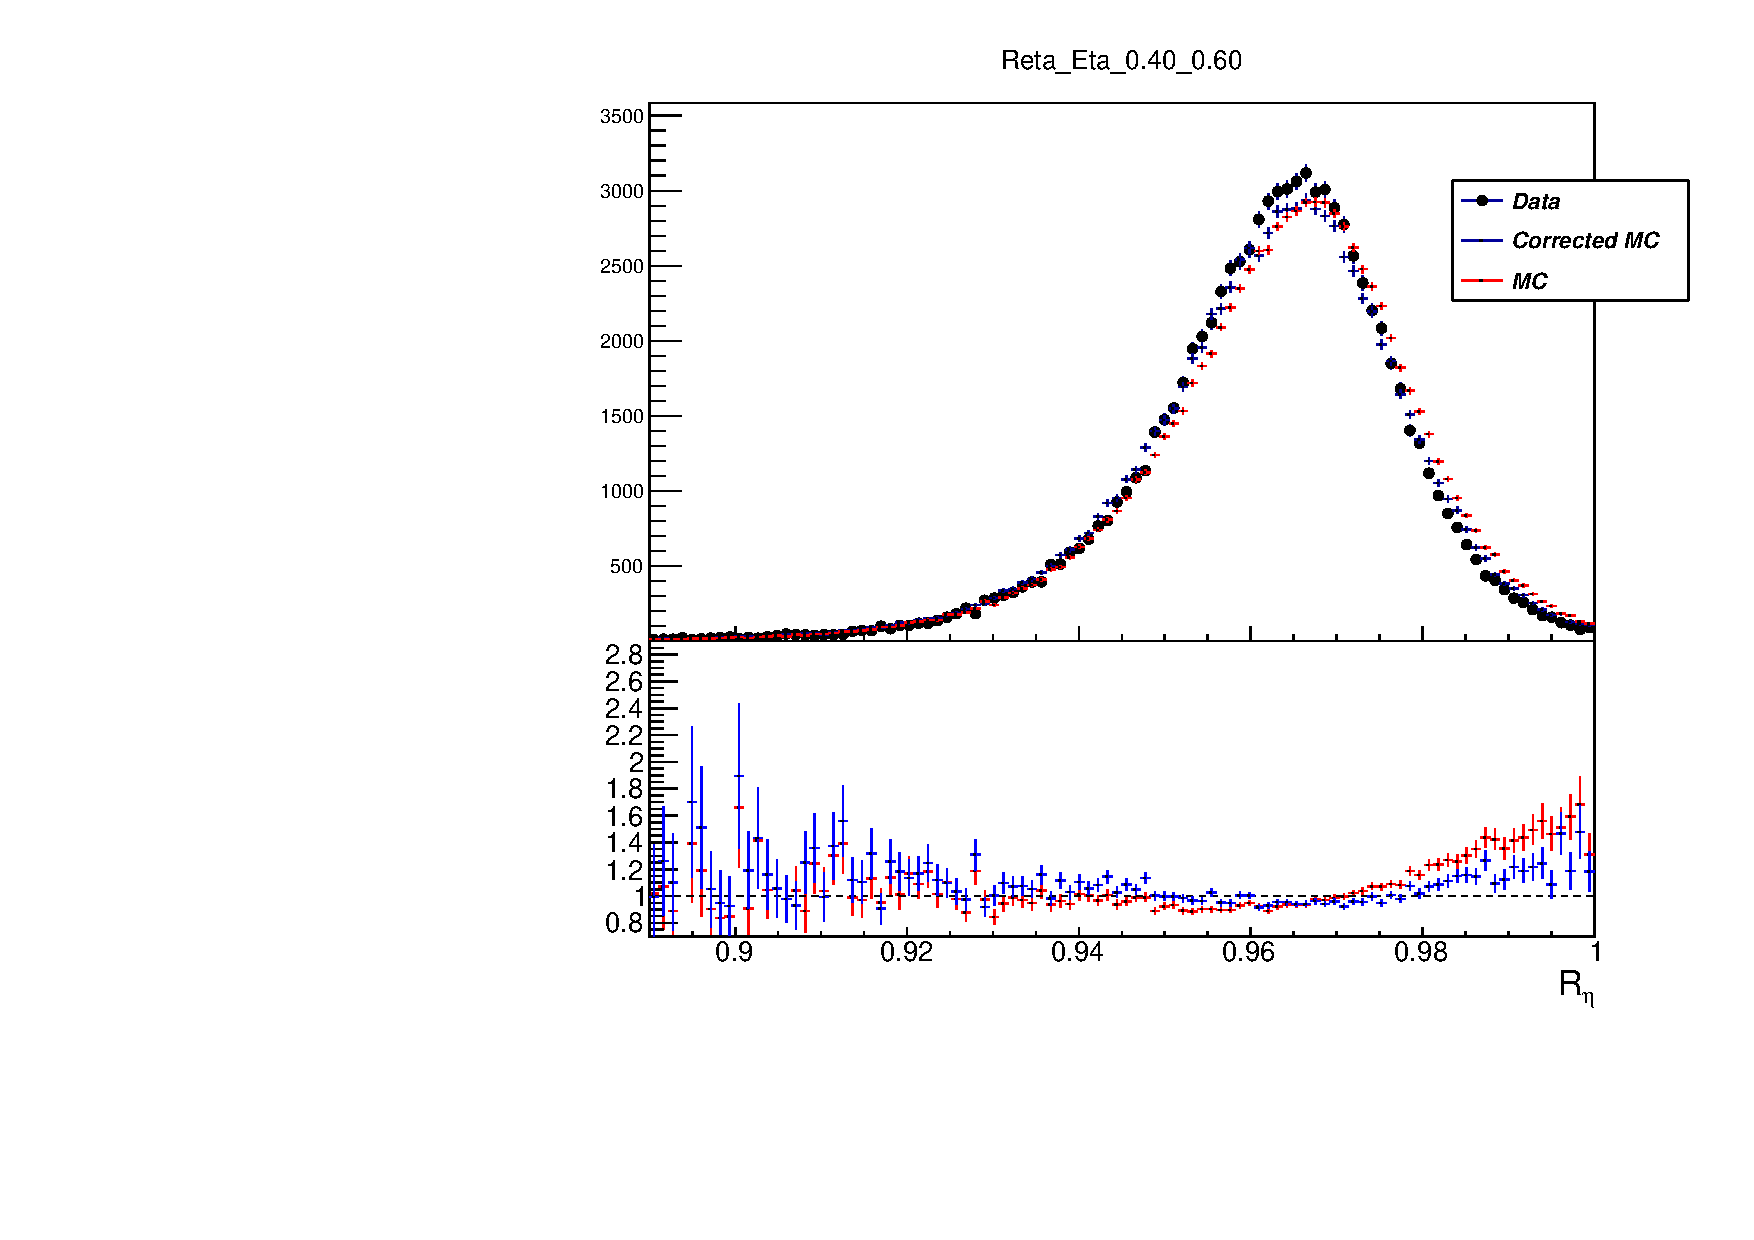
\includegraphics[width=\textwidth,keepaspectratio]{Reta_Eta_4_6_Athena.pdf}
  		\caption{Reweighted  $R_{\eta }$ in $|\eta| = (0.4,0.6)$.  }
  		\label{fig::idreta}
  	\end{subfigure}
  	\hfill
  	\begin{subfigure}[t]{0.5\textwidth} 
  		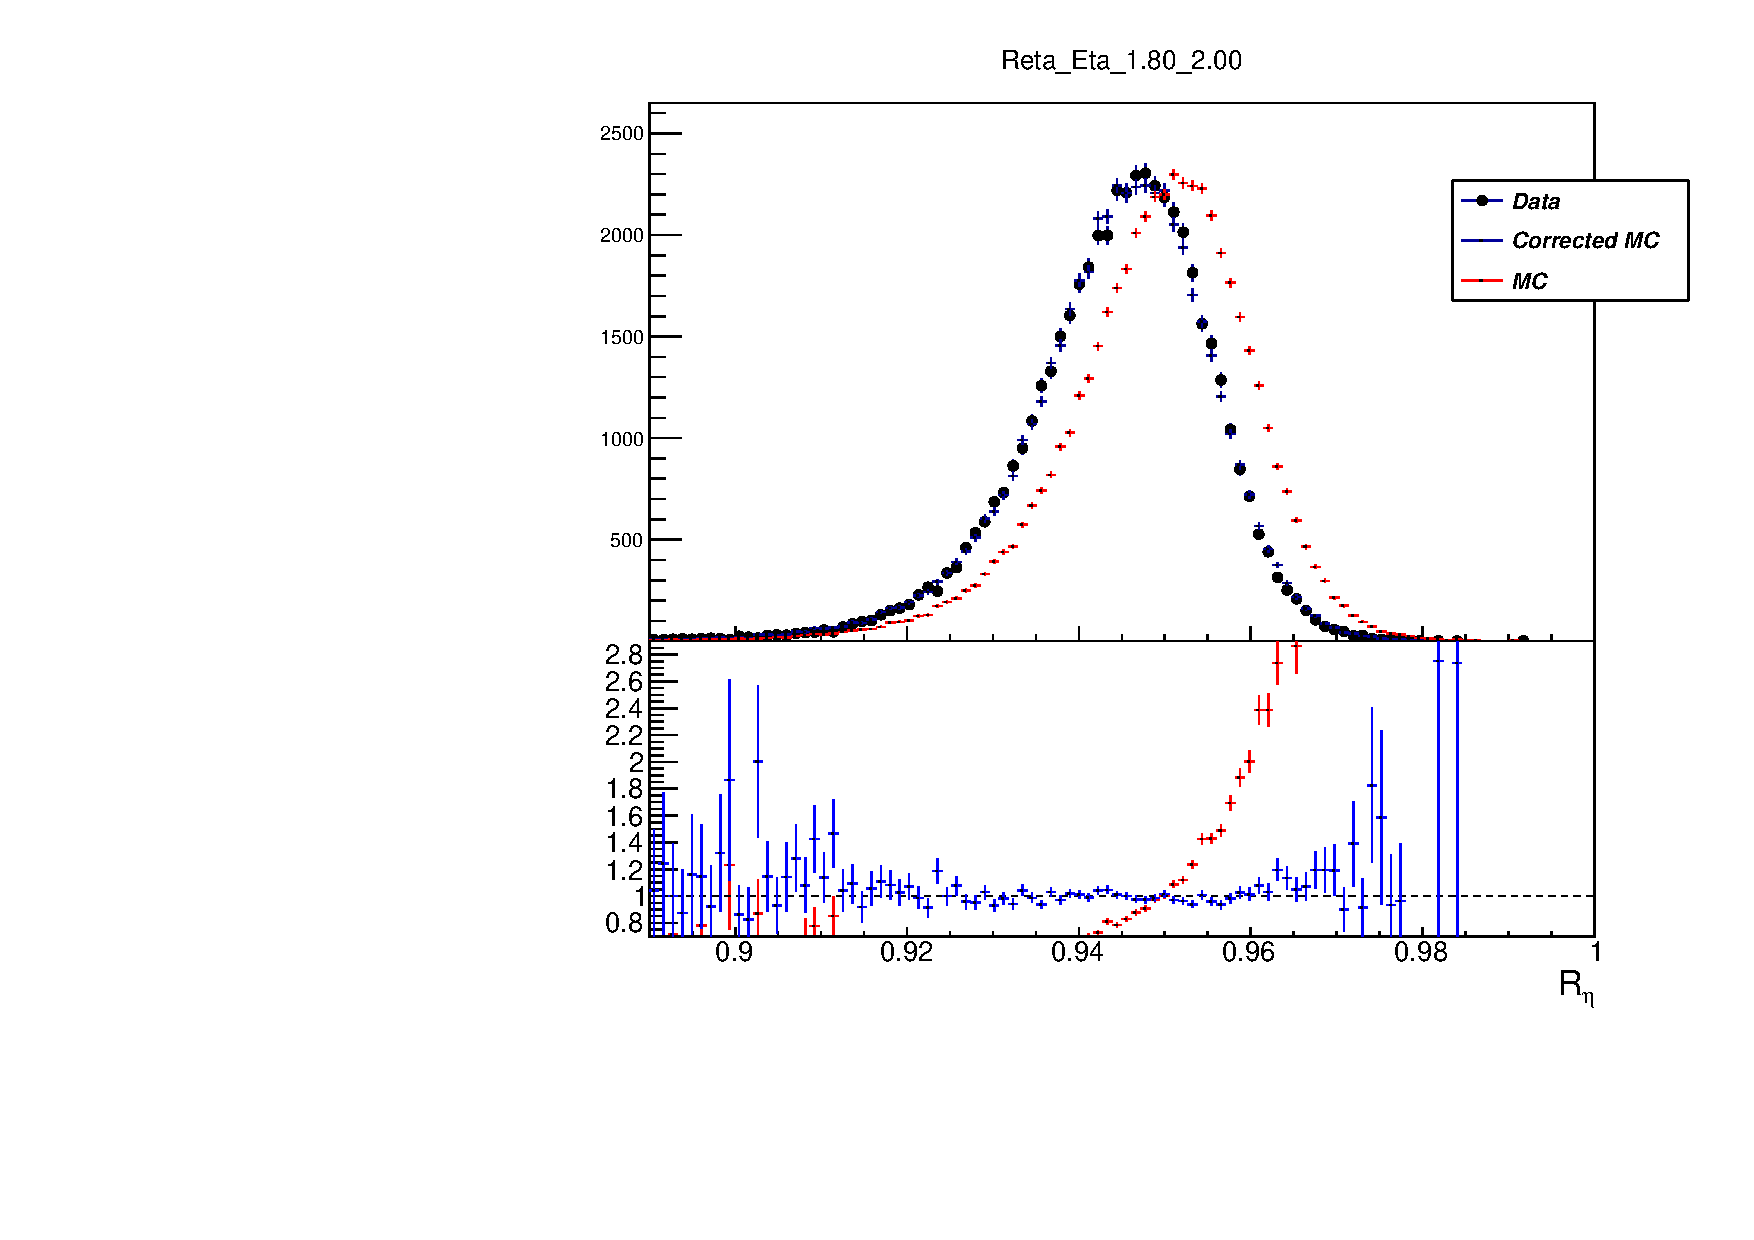
\includegraphics[width=\textwidth,keepaspectratio]{Reta_Eta_18_20_Athena.pdf}
  		\caption{Reweighted  $R_{\eta }$ in $|\eta| = (1.8,2.0)$.  }
  		\label{fig::pdreta}
  	\end{subfigure}
  	\caption{$R_{\eta }$  in the barrel and in the end-cap}
  	\label{fig::reta}
  \end{figure}
 
      \begin{figure}[htbp]
  	\begin{subfigure}[t]{0.5\textwidth}
  		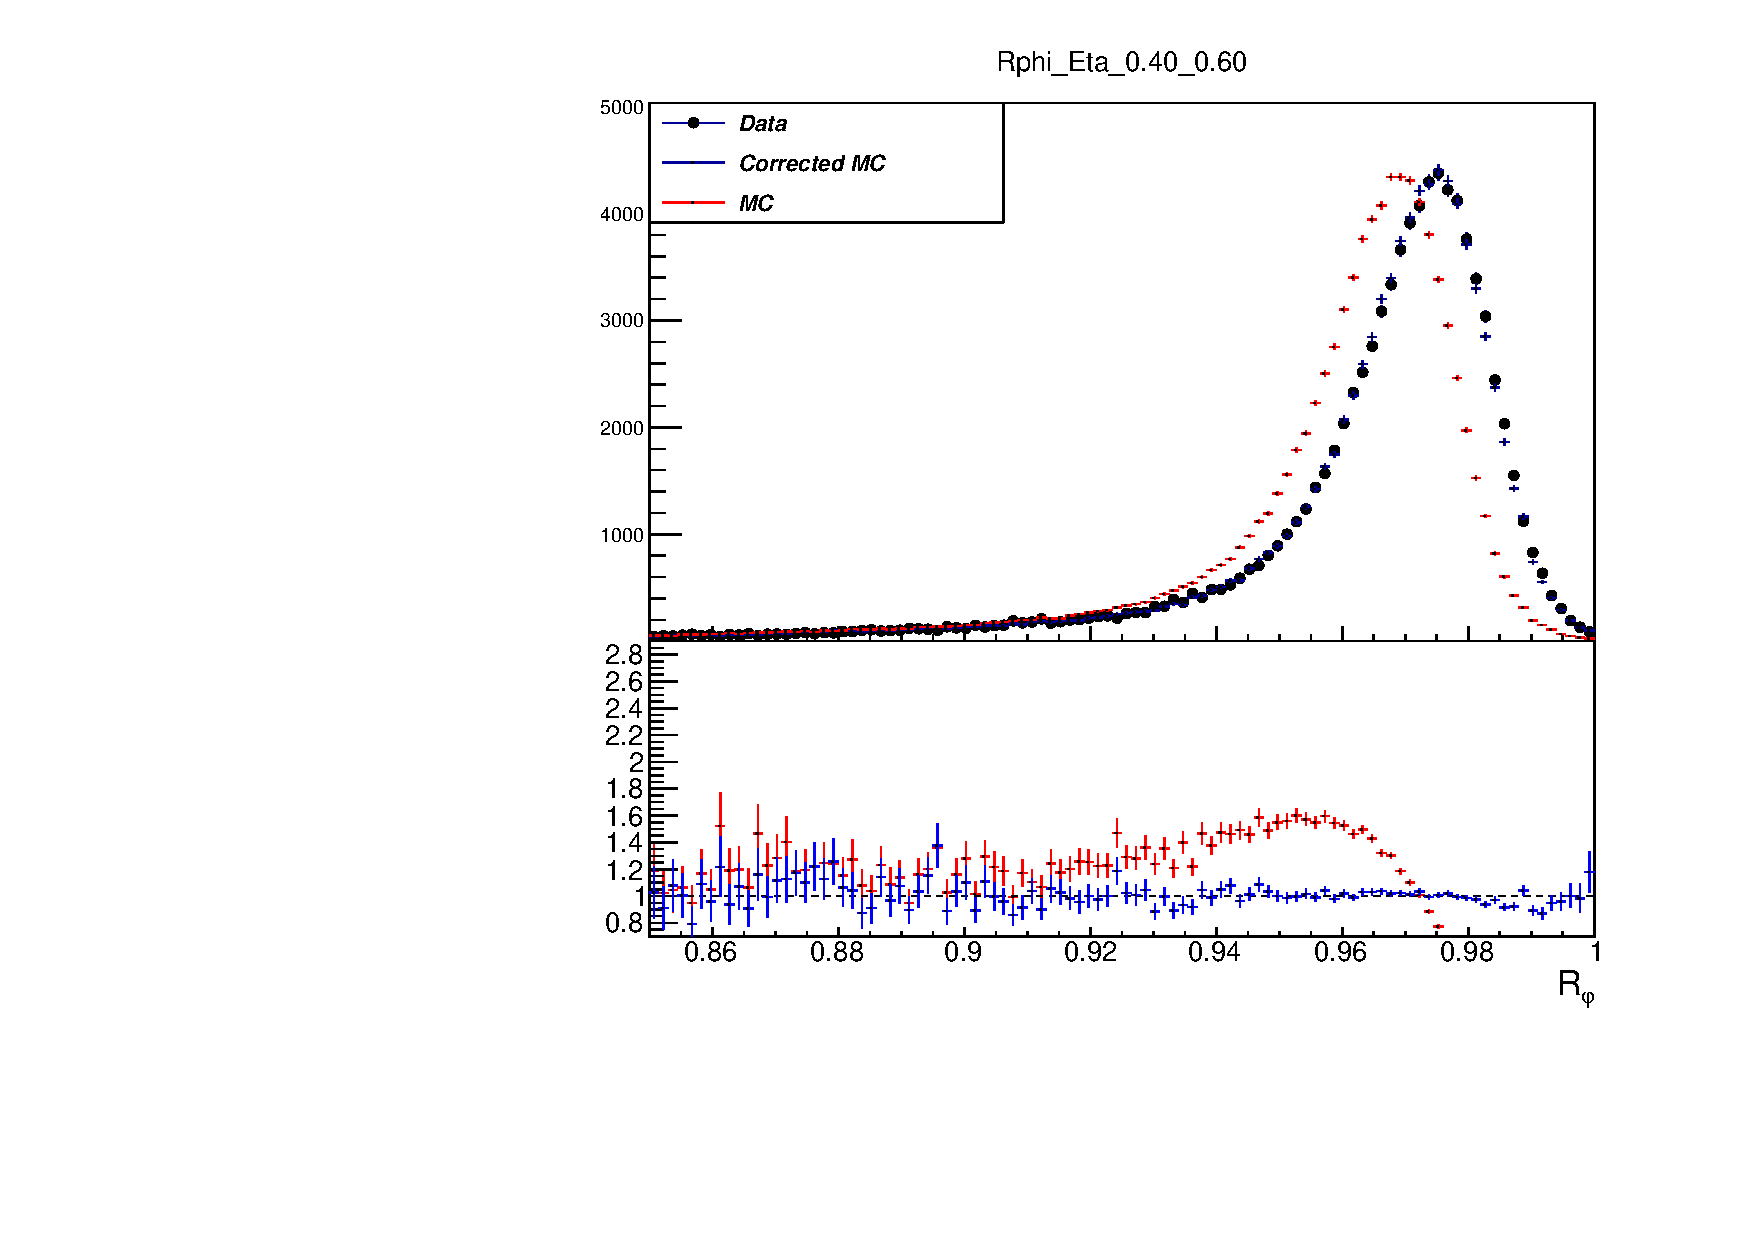
\includegraphics[width=\textwidth,keepaspectratio]{Rphi_Eta_4_6_Athena.pdf}
  		\caption{$R_{\phi}$ in $|\eta| = (0.4,0.6)$ }
  		\label{fig::rphi_rew_04}
  	\end{subfigure}
  	\hfill
  	\begin{subfigure}[t]{0.5\textwidth} 
  		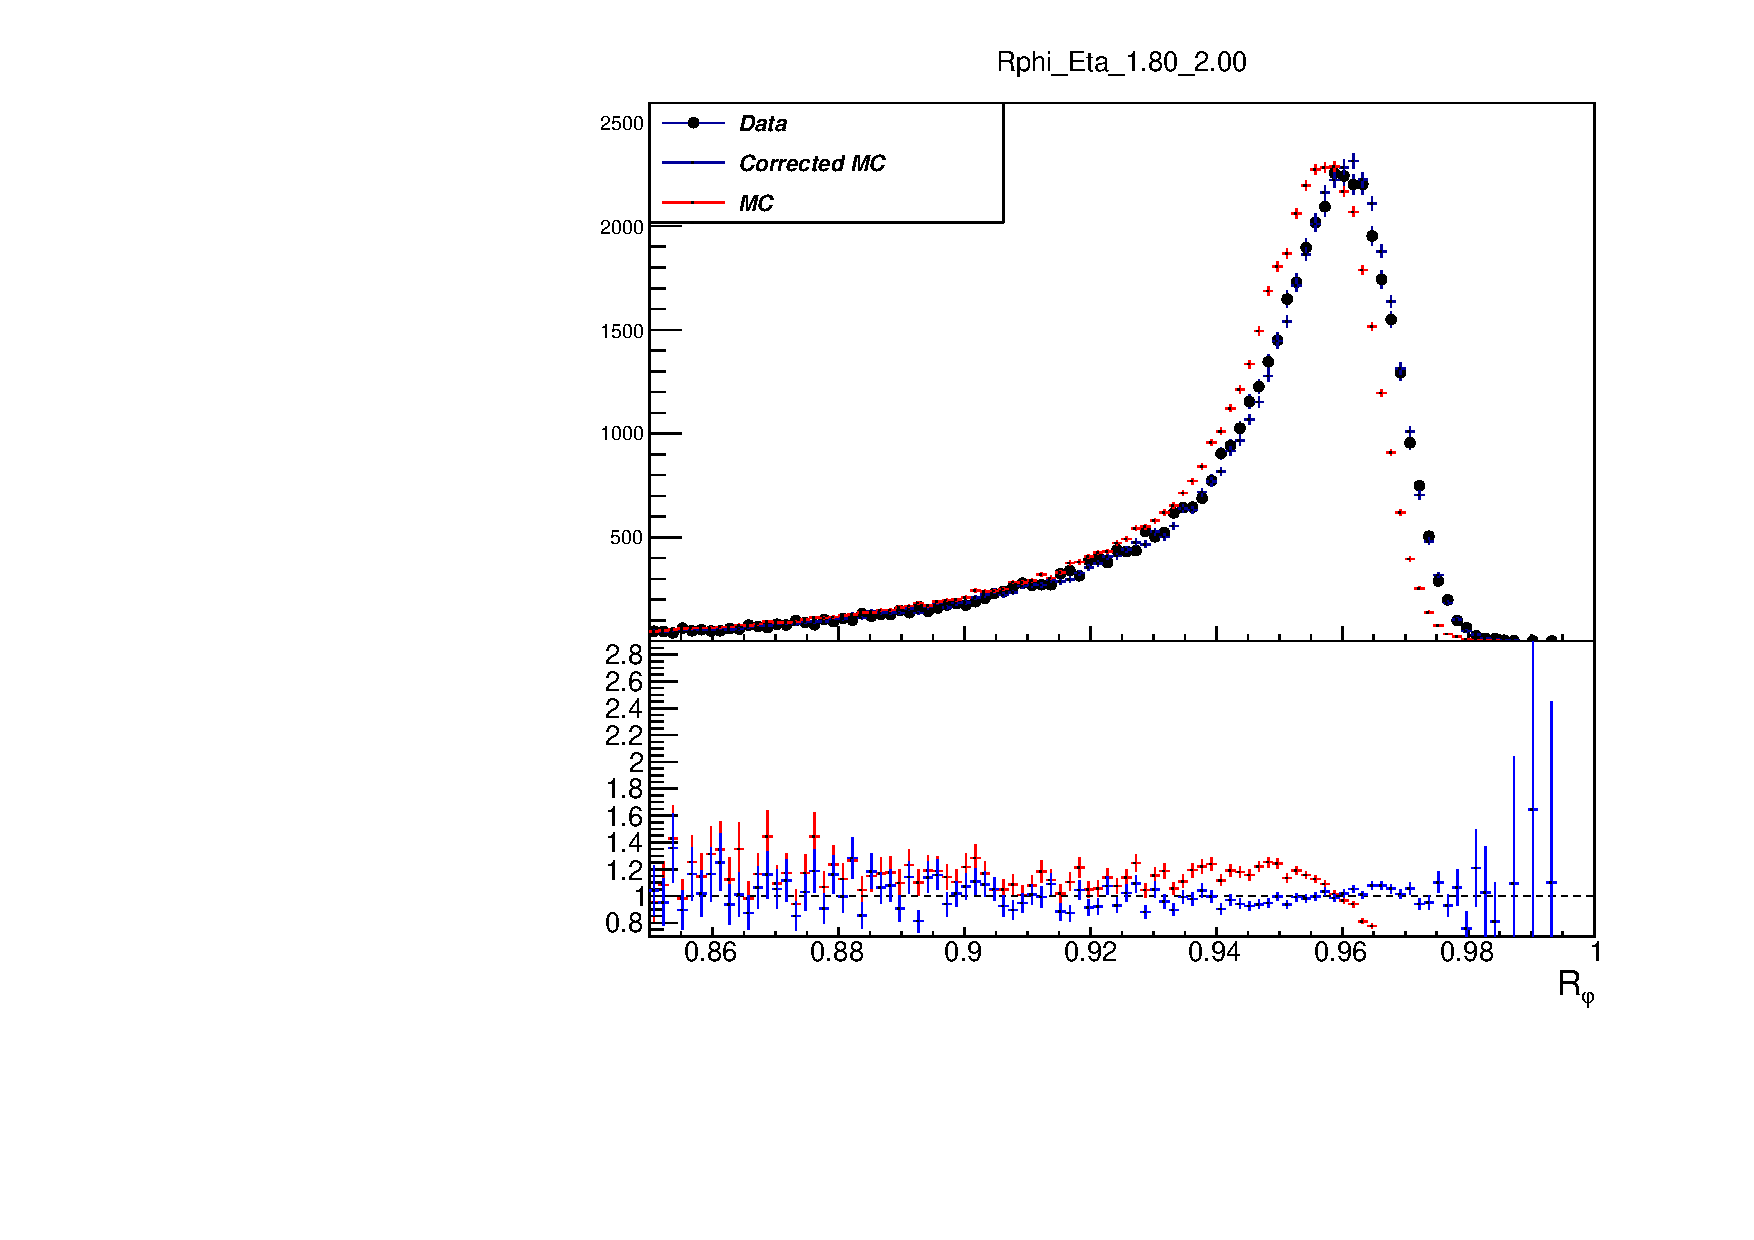
\includegraphics[width=\textwidth,keepaspectratio]{Rphi_Eta_18_20_Athena.pdf}
  		\caption{$R_{\phi}$ in $|\eta| = (1.8,2.0)$ }
  		\label{fig::rphi_rew_18}
  	\end{subfigure}
  	\caption{$R_{\phi}$ in the barel and in the end-cap, Data, MC, reweighted MC}
  	\label{fig::rphi_rew}
  \end{figure}
  
    \begin{figure}[htbp]
	\begin{subfigure}[t]{0.5\textwidth}
		\includegraphics[width=\textwidth,keepaspectratio]{weta2_Eta_4_6_Athena.pdf}
		\caption{$W_{\eta}^2$ in $|\eta| = (0.4,0.6)$ }
		\label{fig::weta2_rew_04}
	\end{subfigure}
	\hfill
	\begin{subfigure}[t]{0.5\textwidth} 
		\includegraphics[width=\textwidth,keepaspectratio]{weta2_Eta_18_20.pdf}
		\caption{$W_{\eta}^2$ in $|\eta| = (1.8,2.0)$ }
		\label{fig::weta2_rew_18}
	\end{subfigure}
	\caption{$W_{\eta}^2$ in the barel and in the end-cap, Data, MC, reweighted MC}
	\label{fig::weta2_rew}
\end{figure}

\begin{figure*}[ht!]
	\subfloat{%
		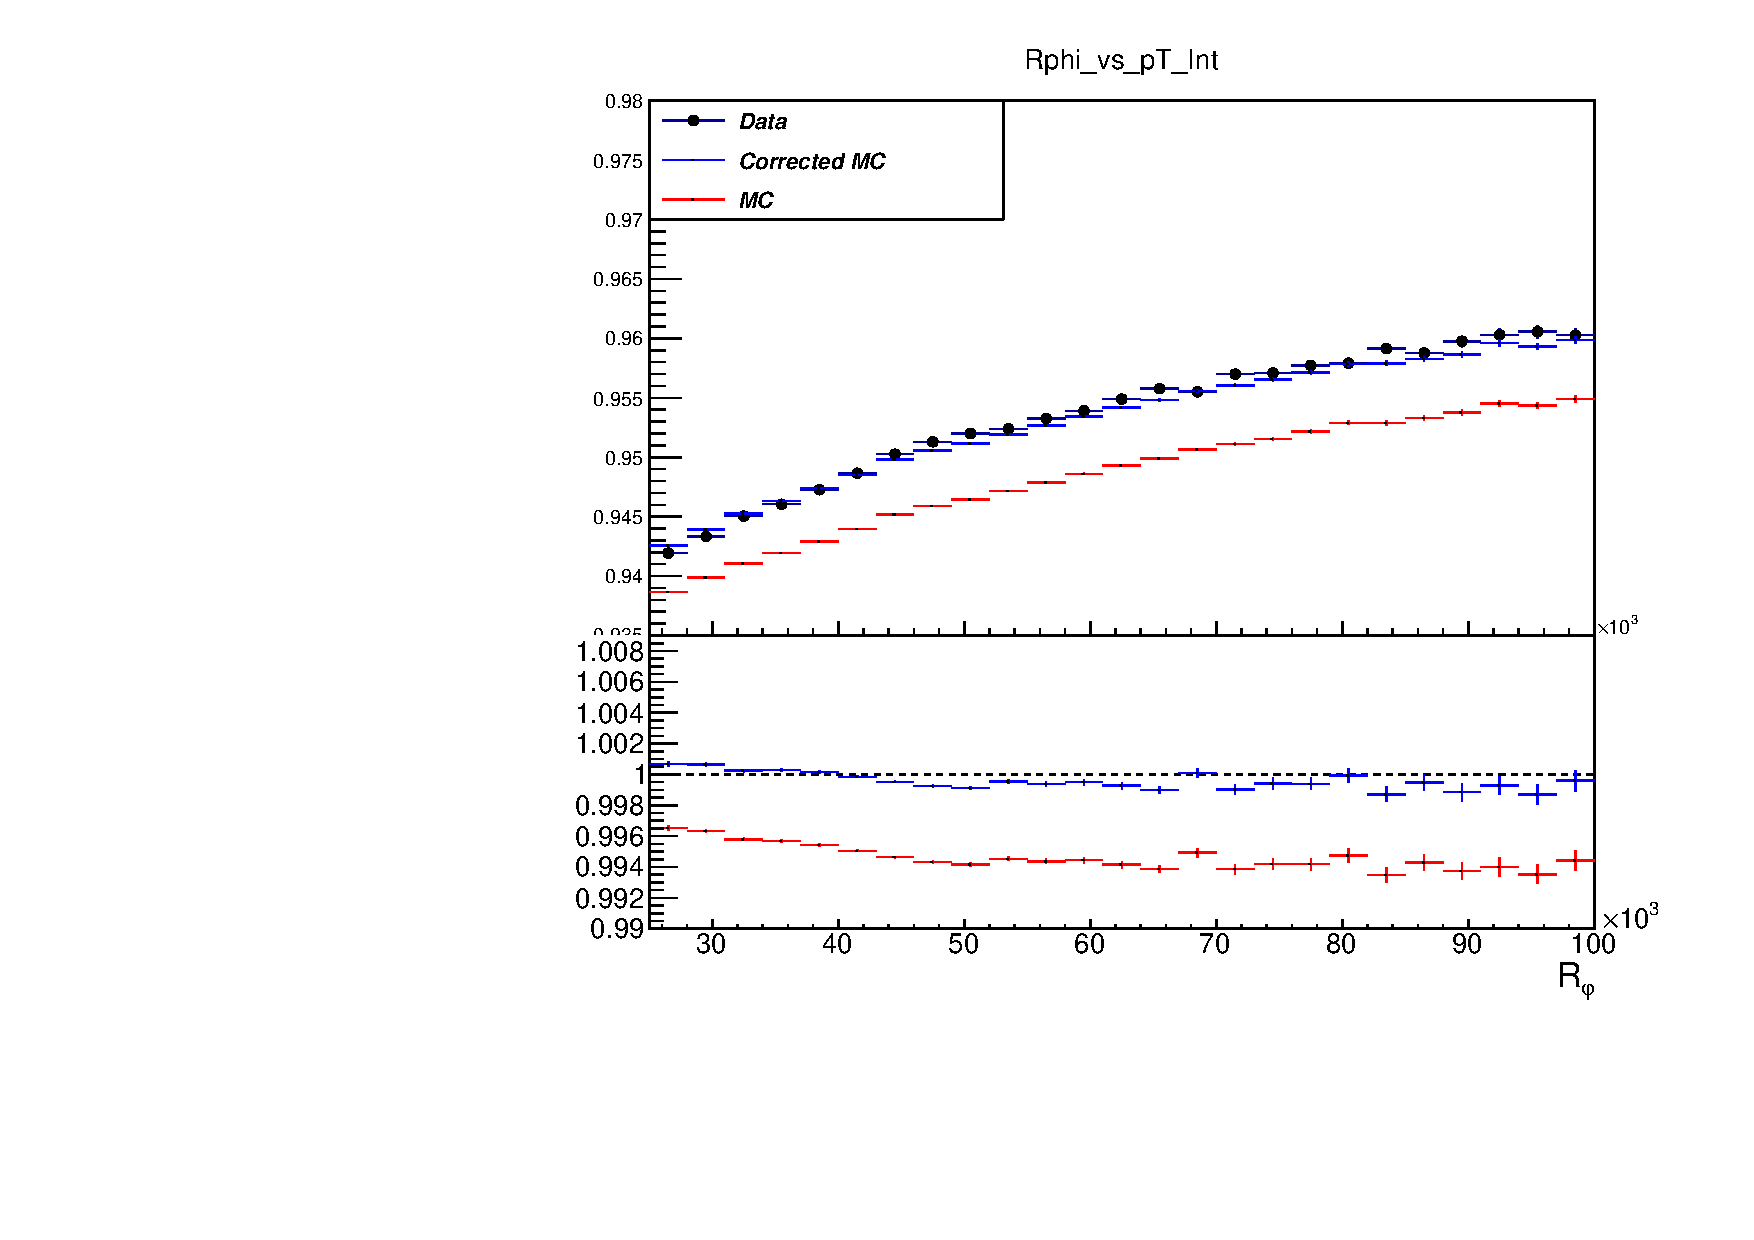
\includegraphics[width=0.33\textwidth]{Rphi_vs_pT_Int}}
	\quad
	\subfloat {%
		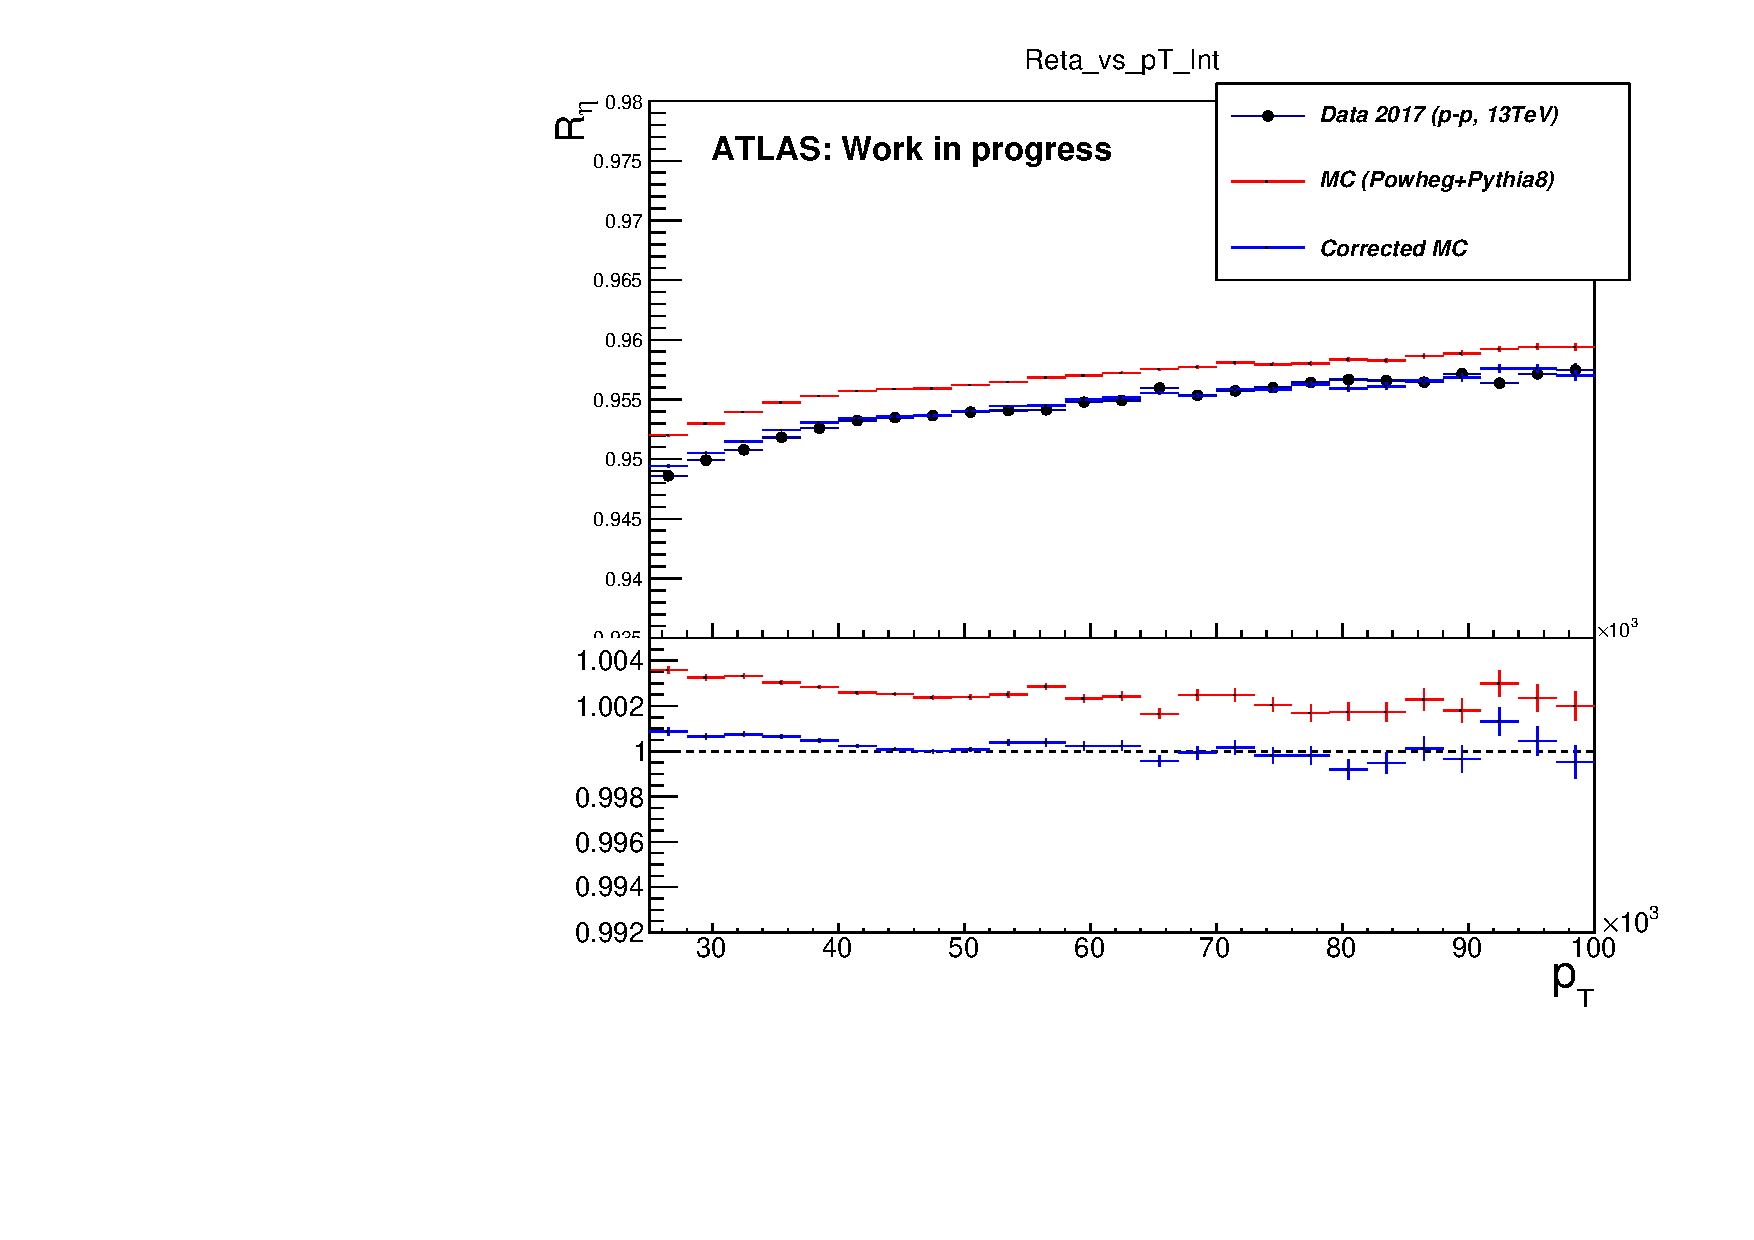
\includegraphics[width=0.33\textwidth]{Reta_vs_pT_Int}}
	\quad
	\subfloat{%
		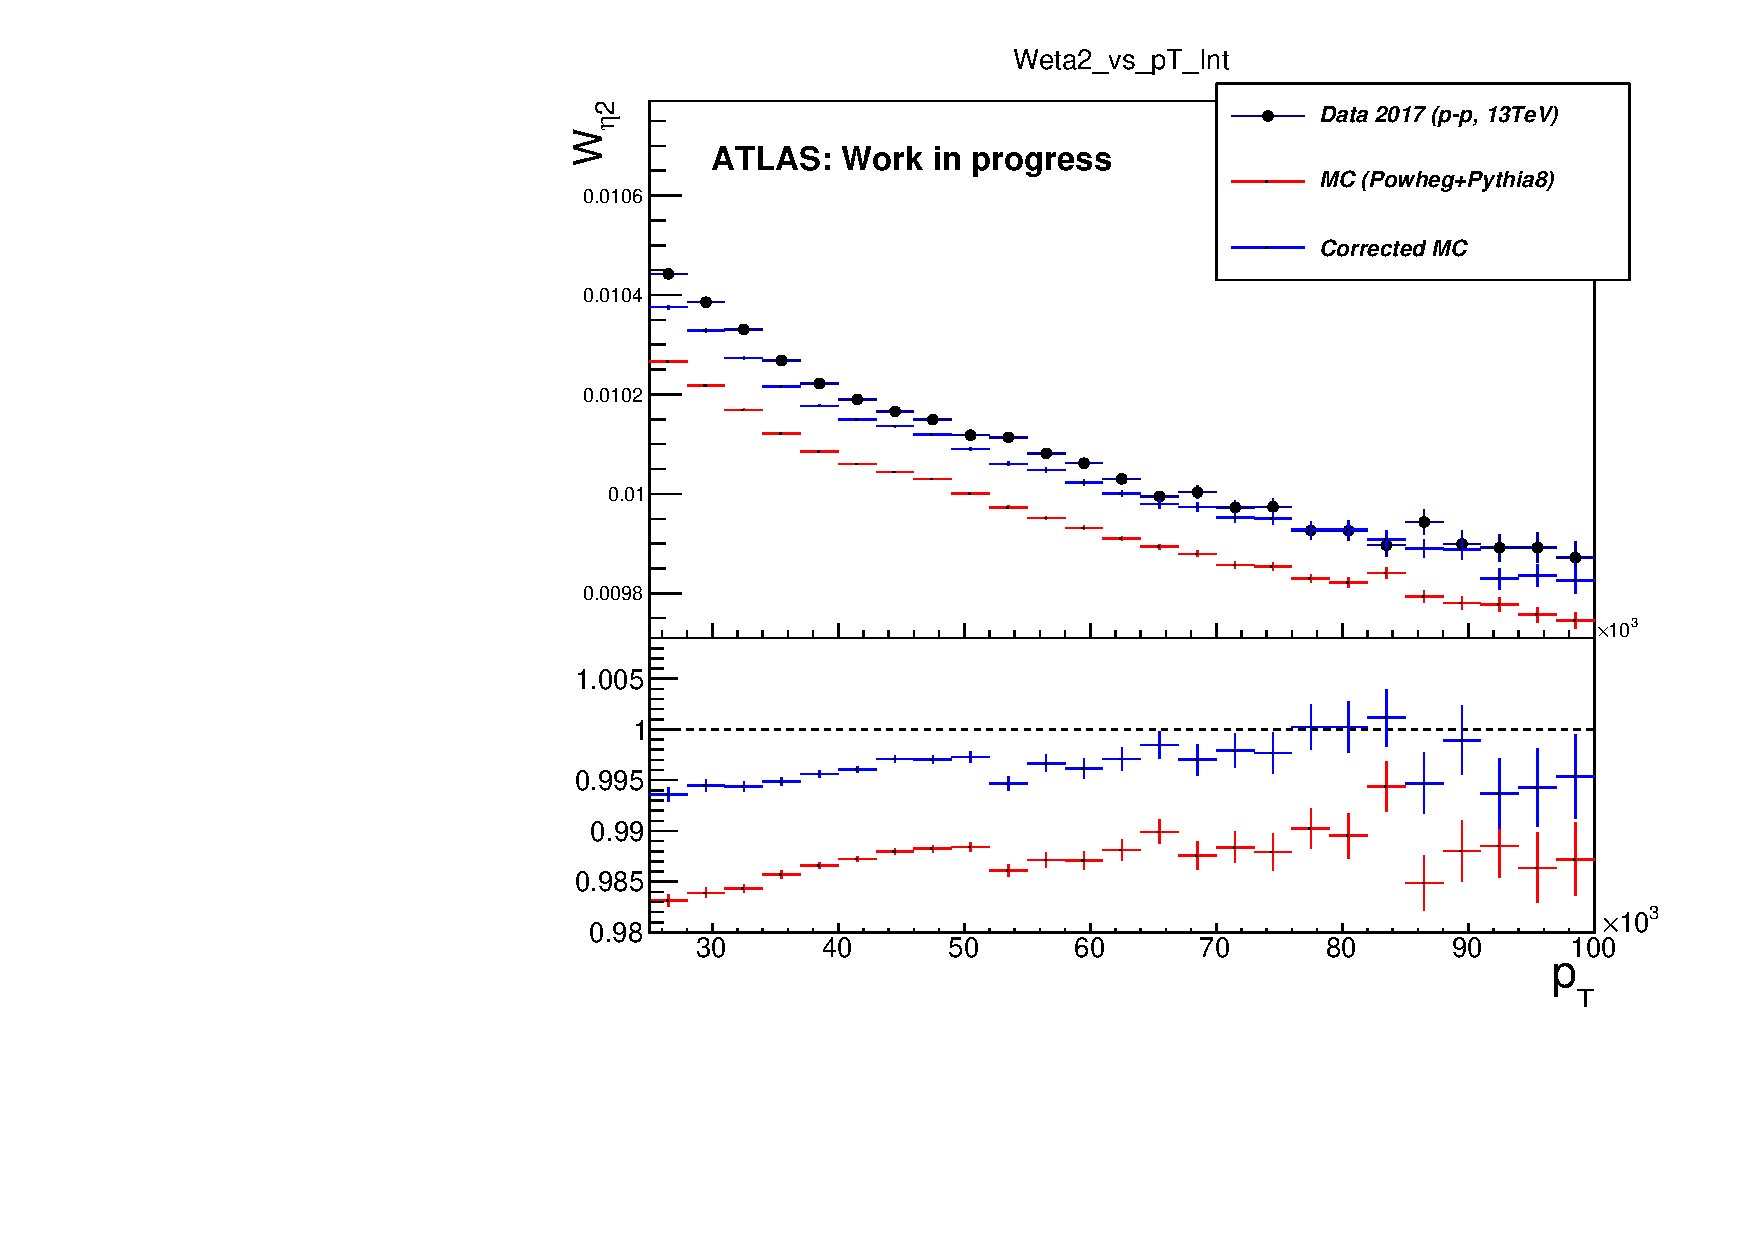
\includegraphics[width=0.33\textwidth]{Weta2_vs_pT_Int}}\\

	\caption{ 	\label{fig::integrated} Distributions integrated over pT (a) $R_{\phi}$; (b) $R_{\eta}$; (c)$W_{\eta 2}$.}
\end{figure*}


  
  \begin{figure}[htbp]
  	\centering
  	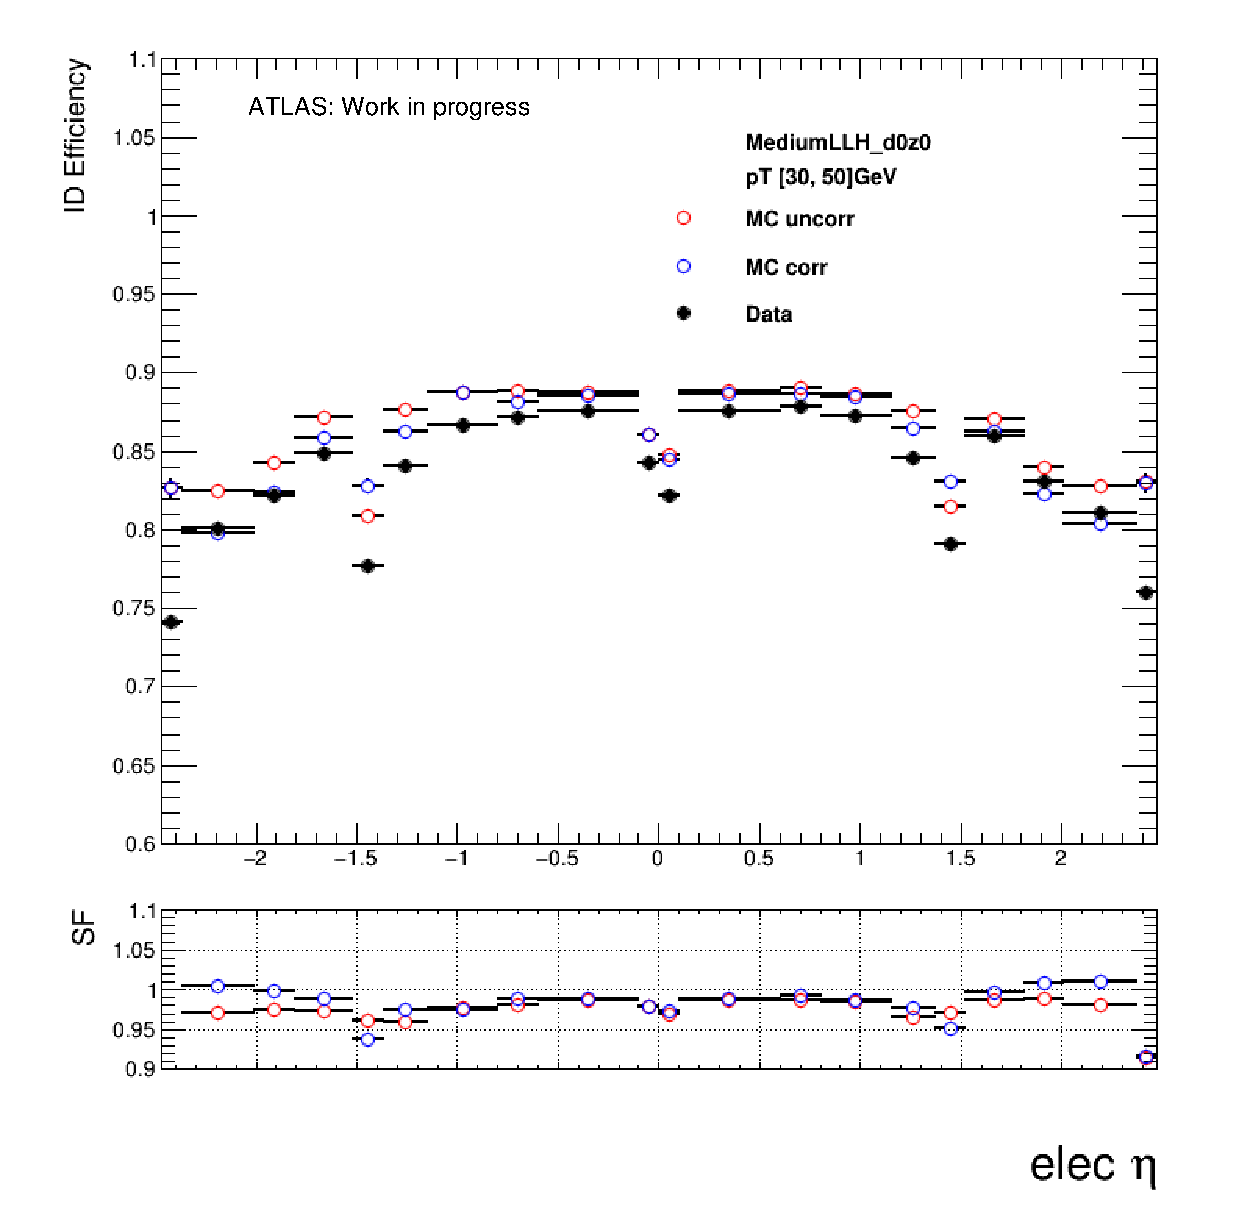
\includegraphics[width=0.99\textwidth,keepaspectratio]{MCeffm247tom237.pdf}\\
  	\caption{Electron identification efficiency as a function of the electron pseudo-rapidity}
  	\label{fig::SF}
  \end{figure}
  \section{Appendix: control plots}

  \begin{figure*}[ht!]
  	\subfloat{%
  		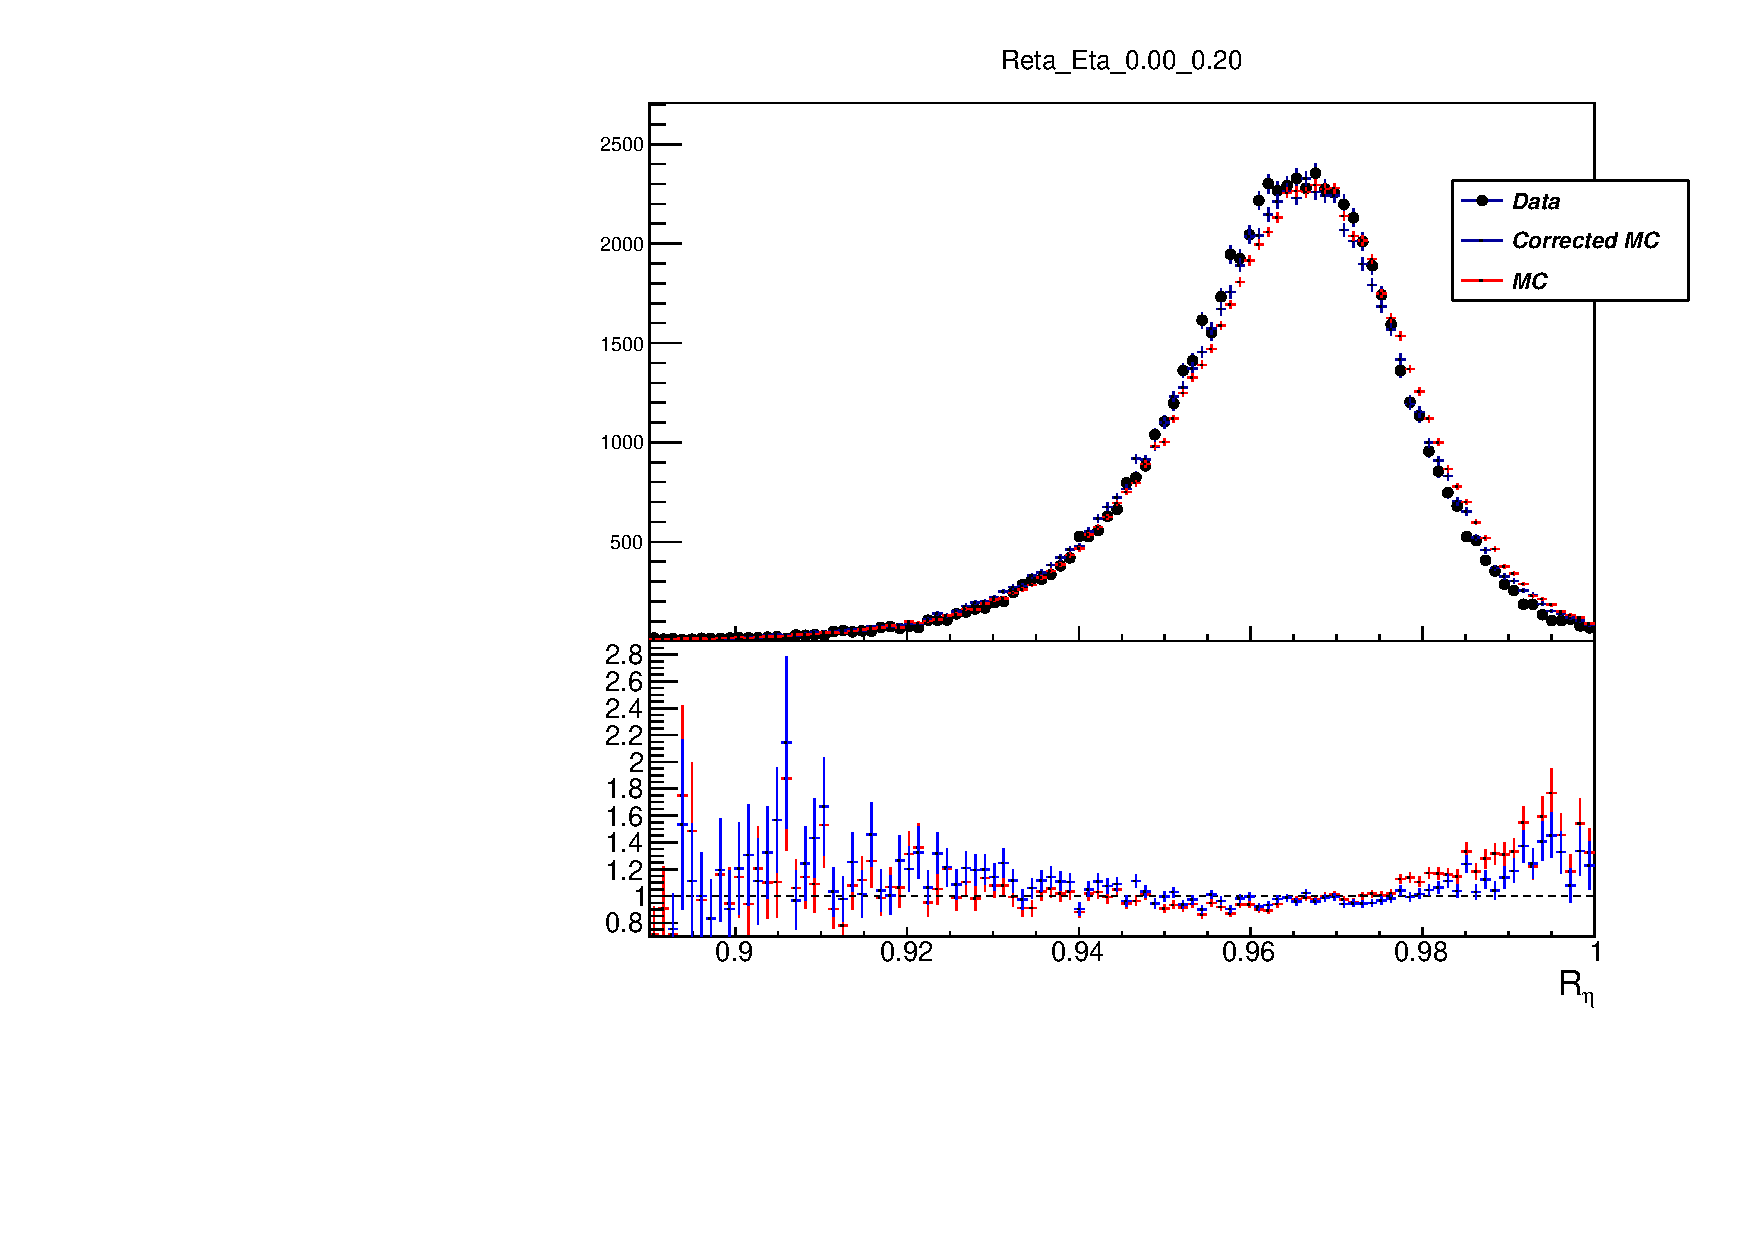
\includegraphics[width=0.33\textwidth]{Reta_Eta_0_2_Athena}}
  	\quad
  	\subfloat {%
  		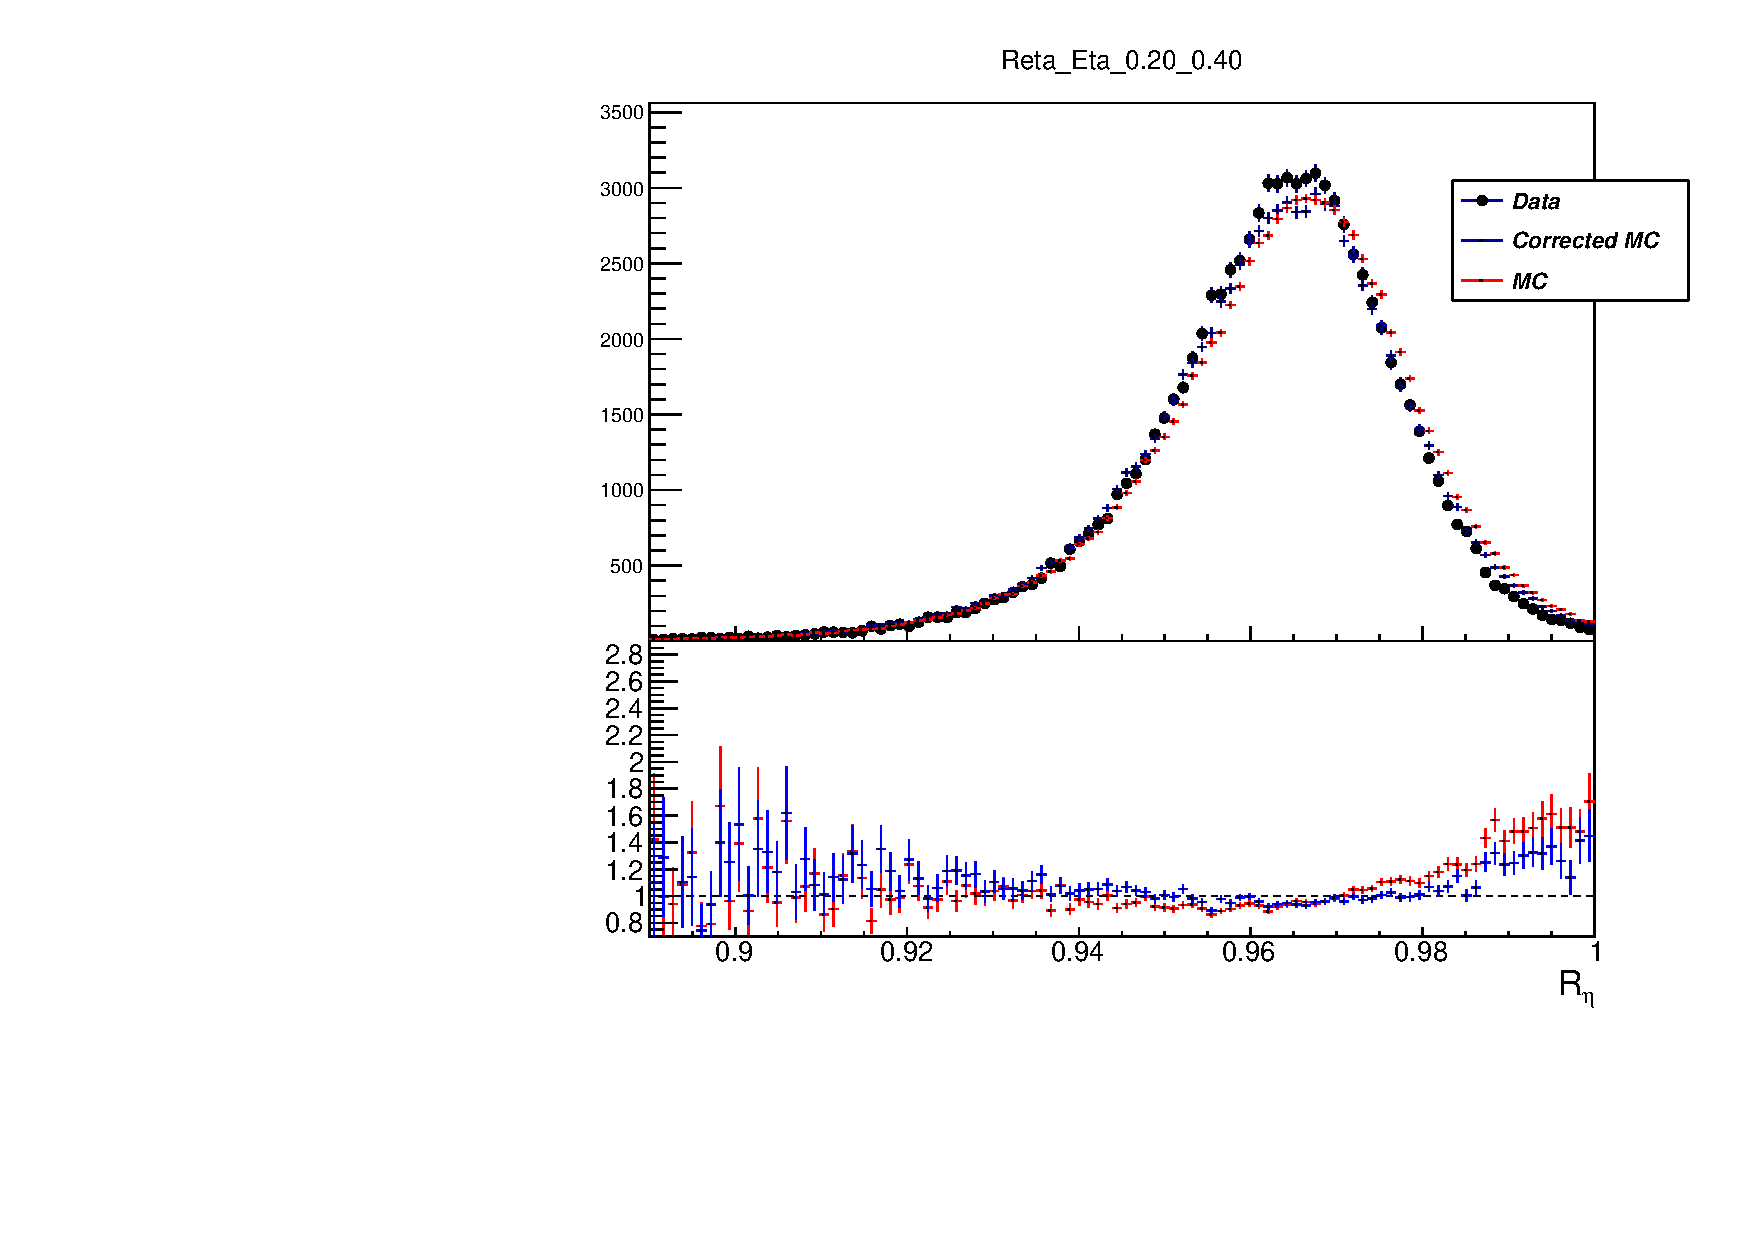
\includegraphics[width=0.33\textwidth]{Reta_Eta_2_4_Athena}}
  	\quad
  	\subfloat{%
  		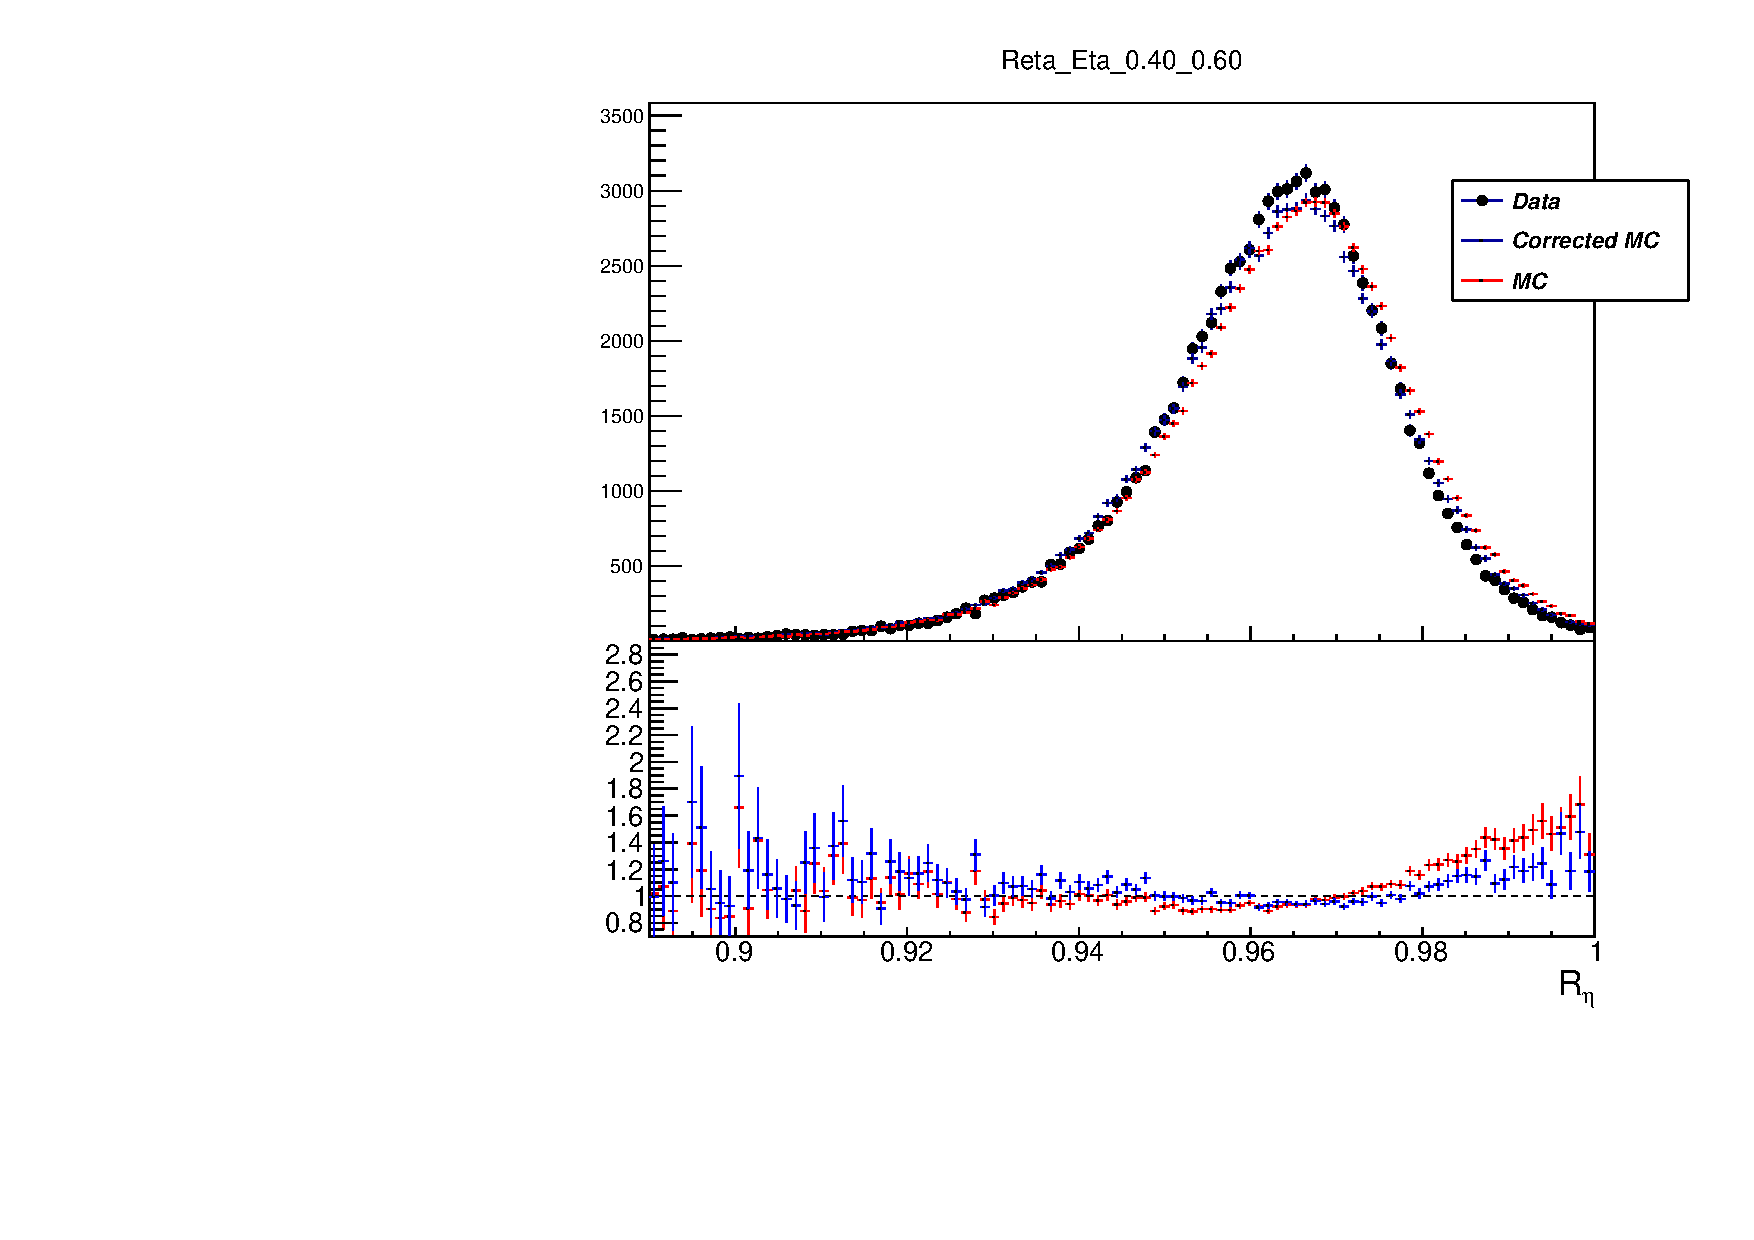
\includegraphics[width=0.33\textwidth]{Reta_Eta_4_6_Athena}}\\
  	\subfloat{%
  		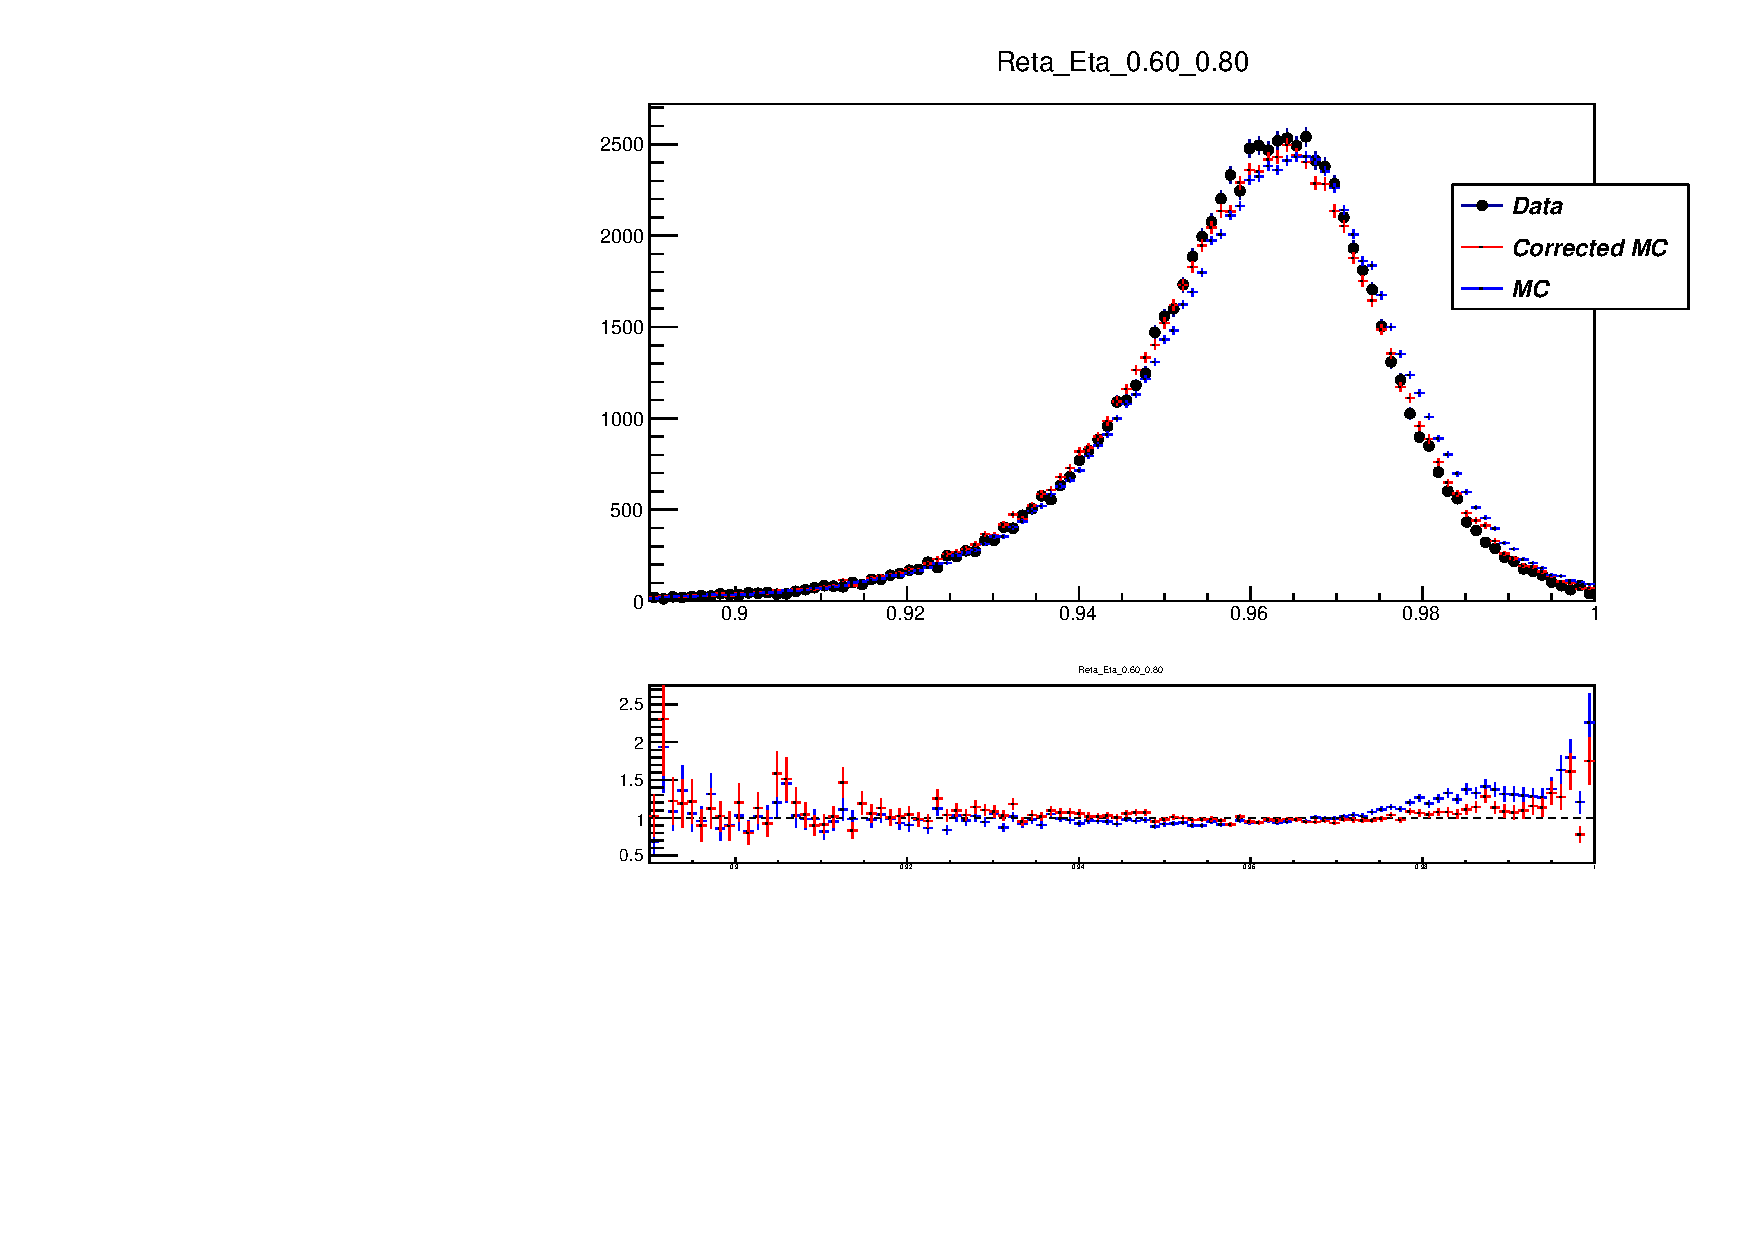
\includegraphics[width=0.33\textwidth]{Reta_Eta_6_8_Athena}}
  	\quad
  	\subfloat {%
  		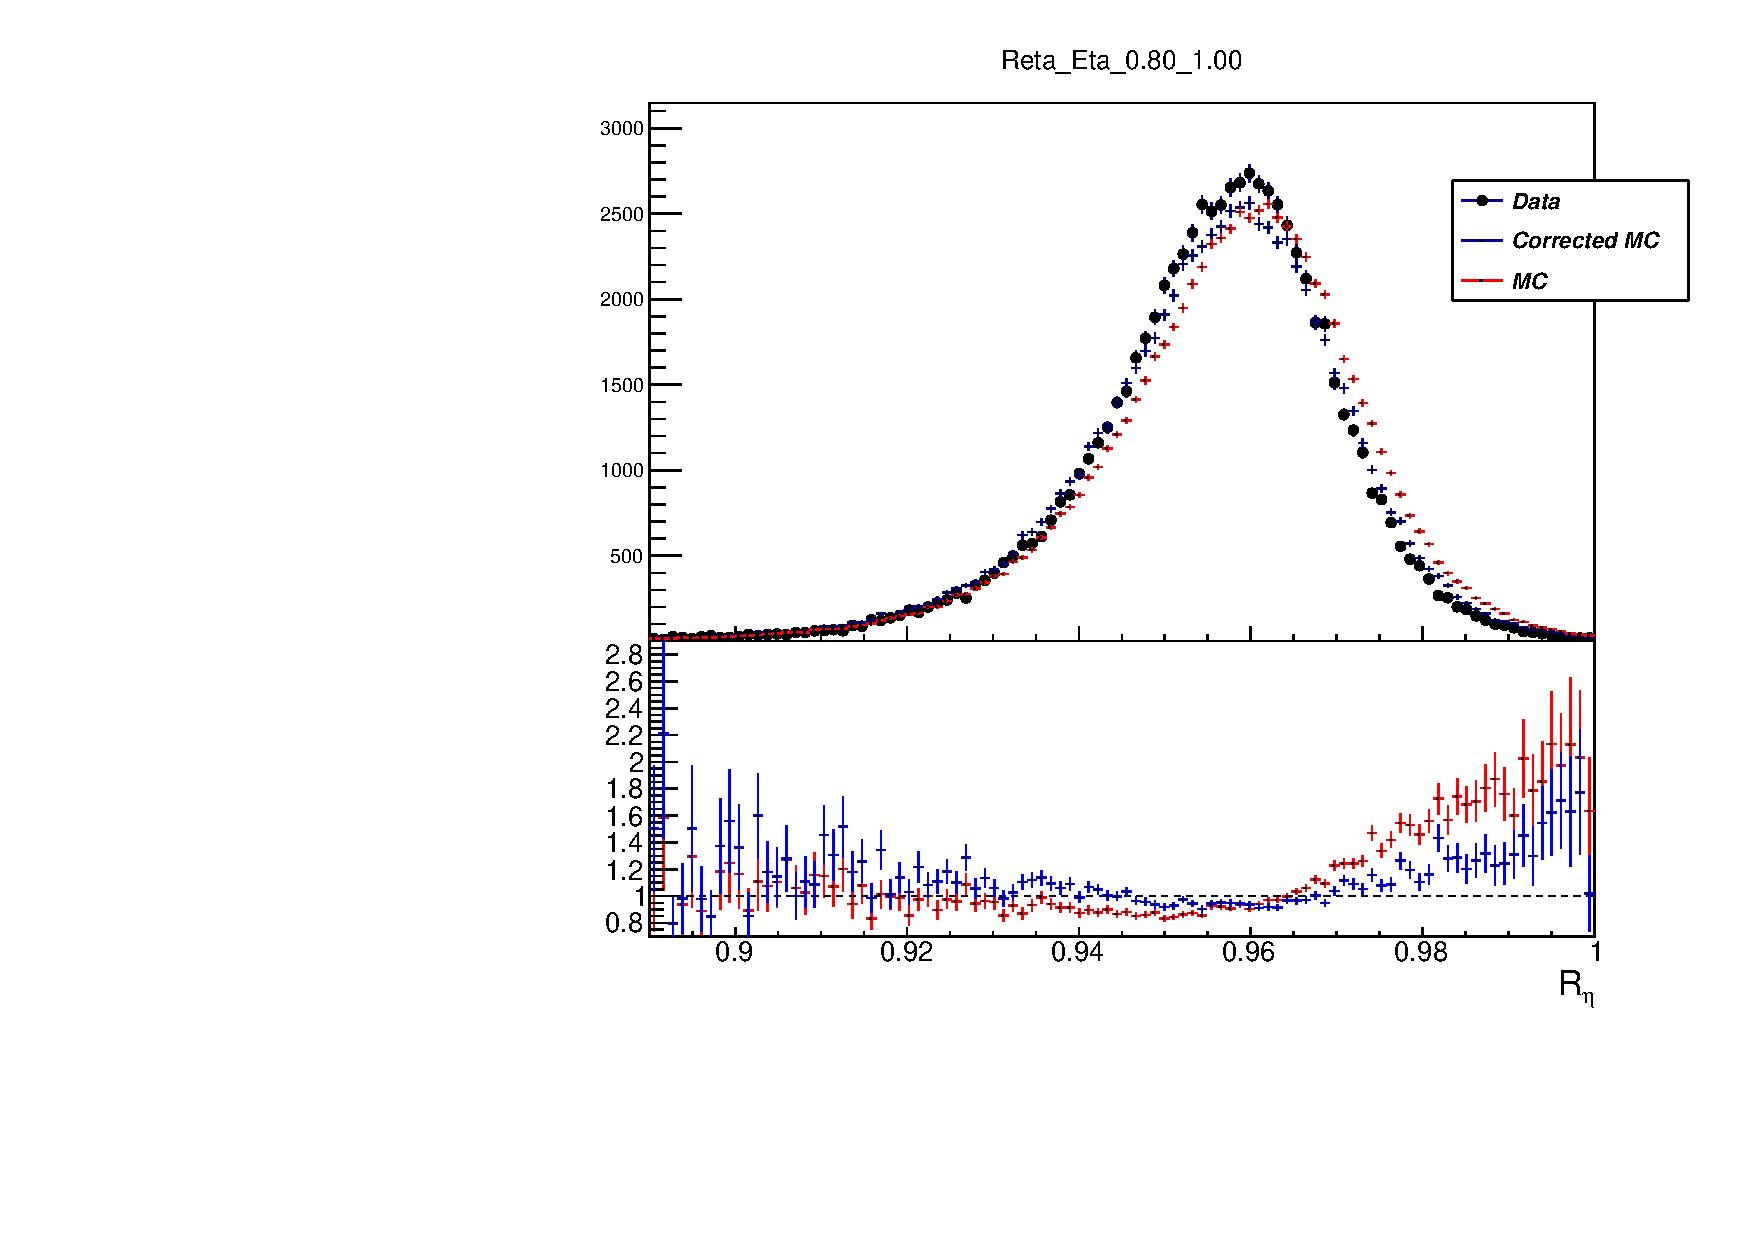
\includegraphics[width=0.33\textwidth]{Reta_Eta_8_10_Athena}}
  	\quad
  	\subfloat{%
  		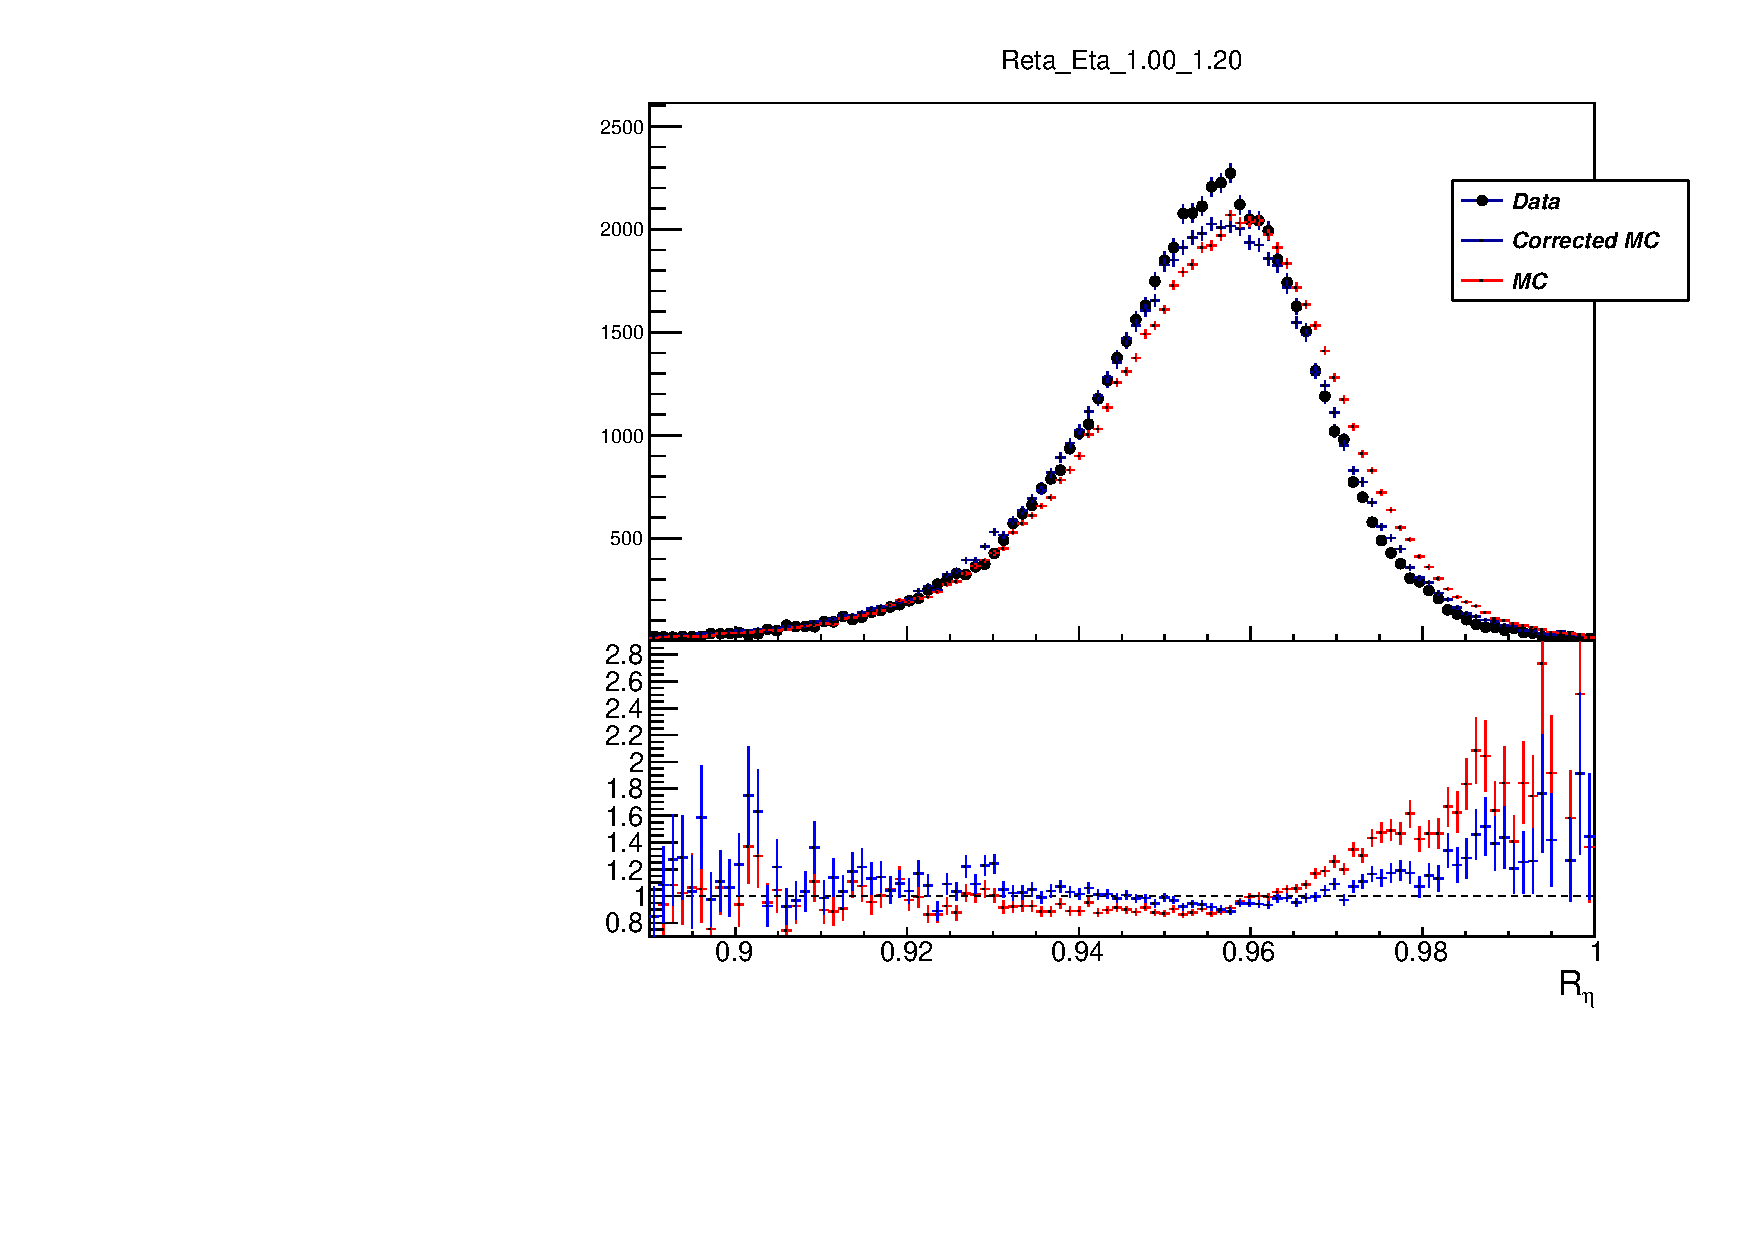
\includegraphics[width=0.33\textwidth]{Reta_Eta_10_12_Athena}}\\
	\subfloat{%
		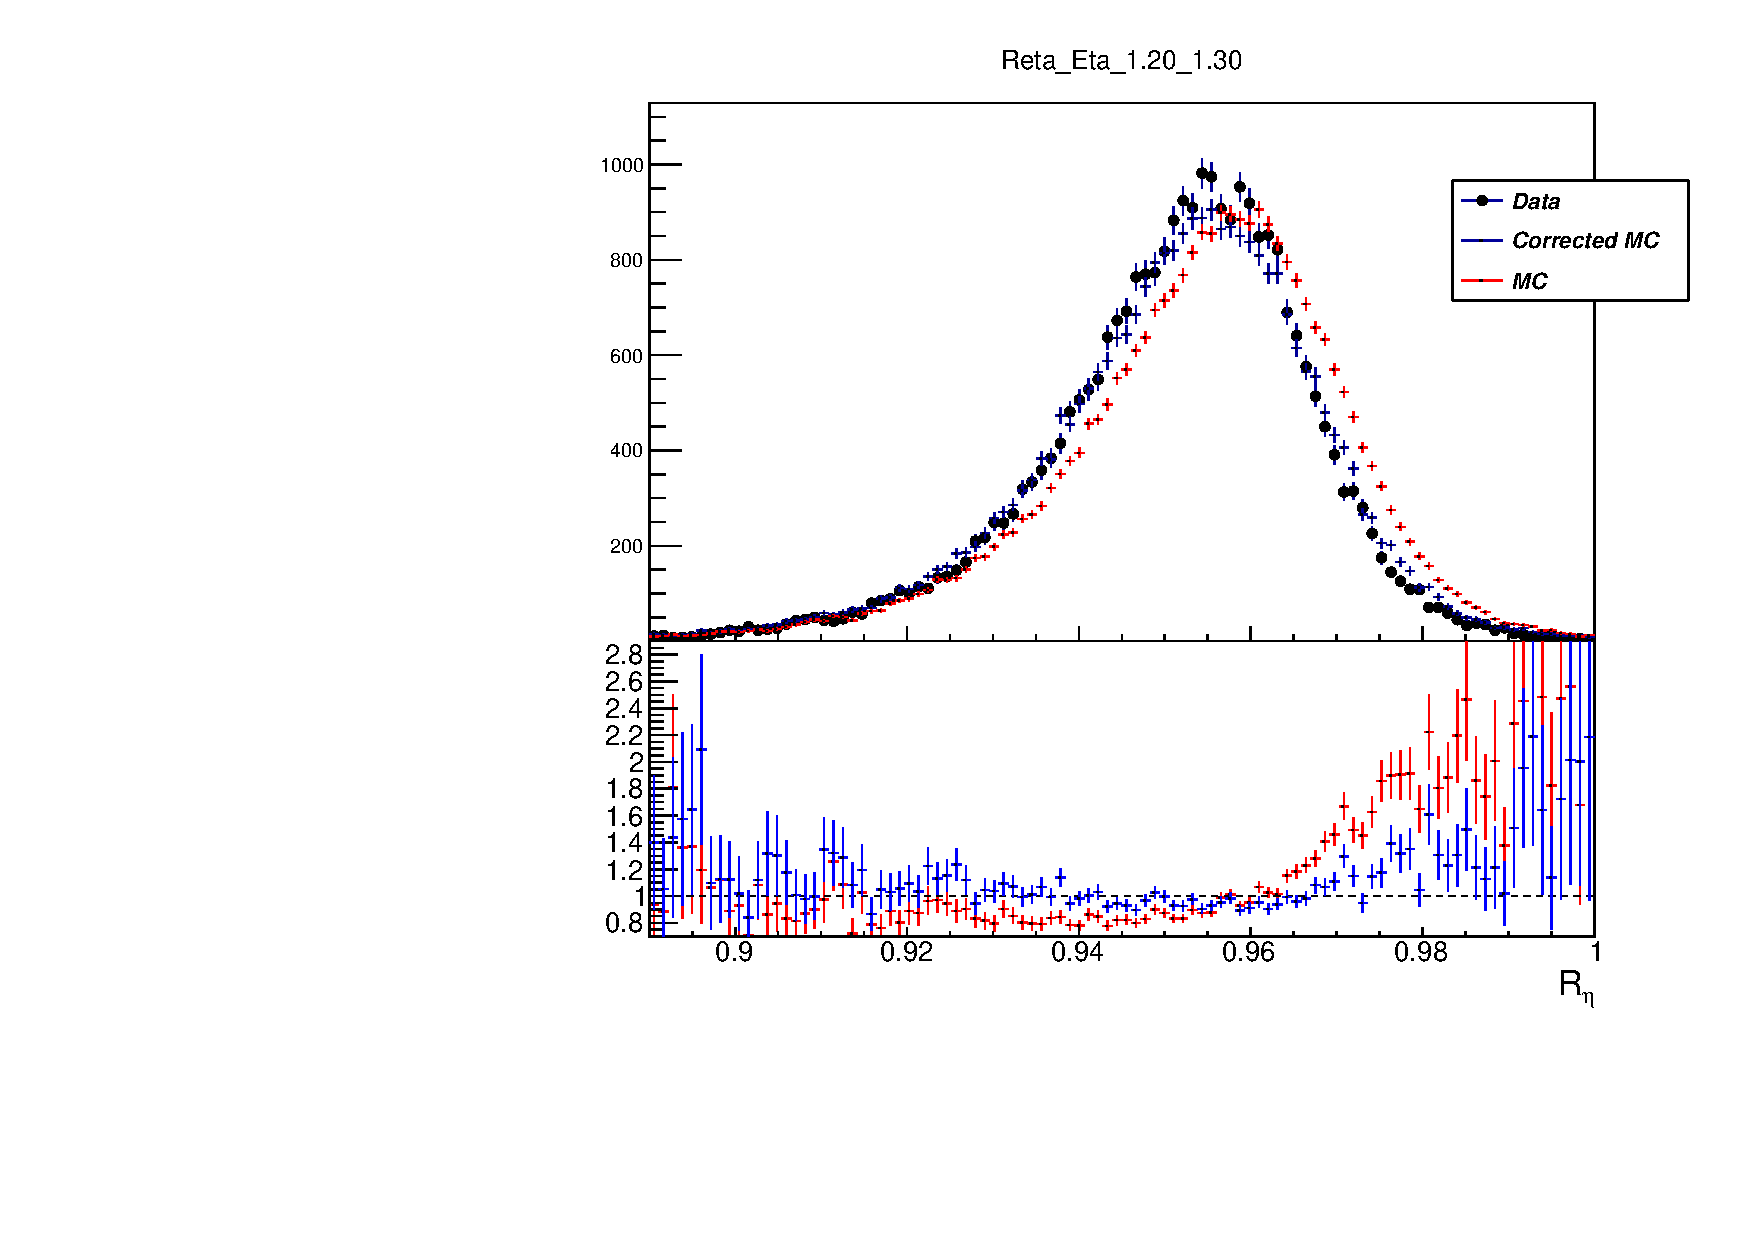
\includegraphics[width=0.33\textwidth]{Reta_Eta_12_13_Athena}}
	\quad
	\subfloat{%
		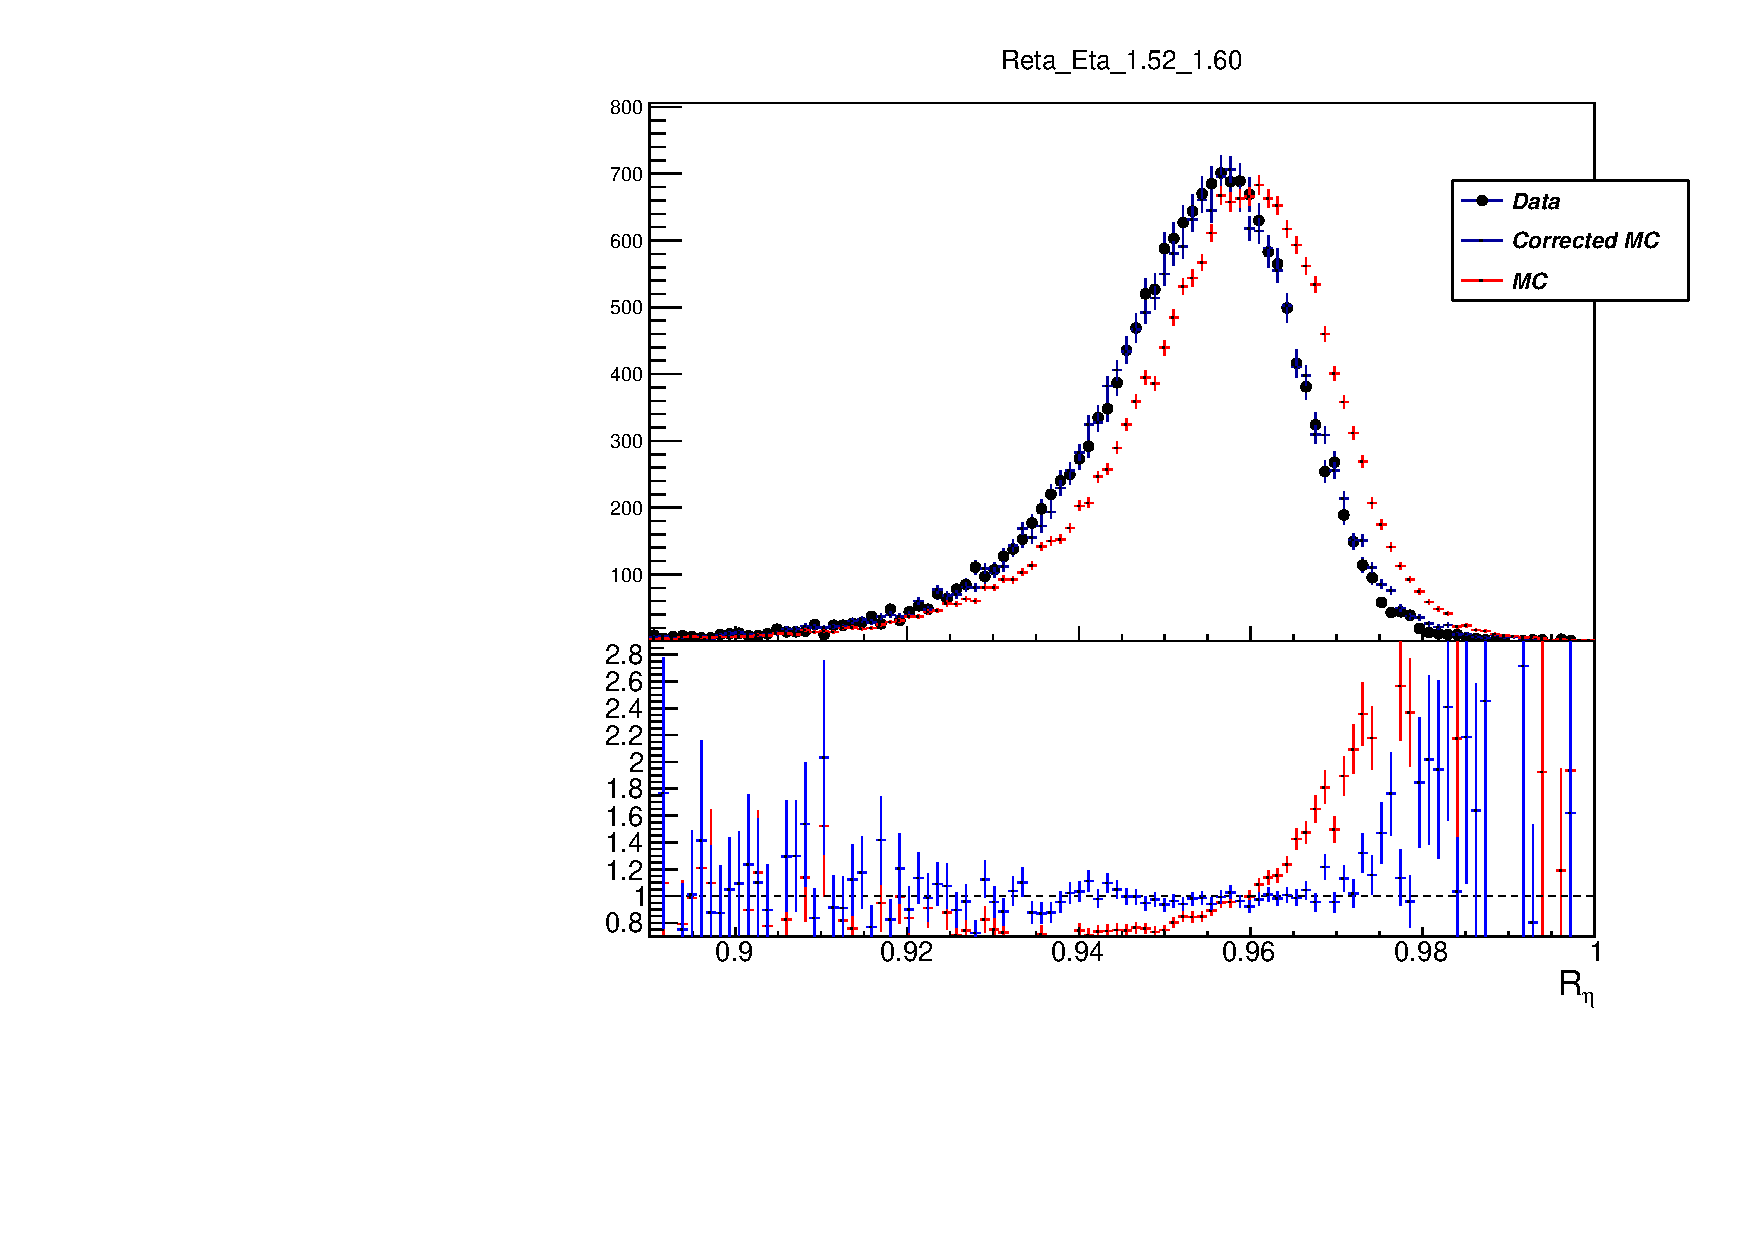
\includegraphics[width=0.33\textwidth]{Reta_Eta_152_16_Athena}}
	\subfloat{%
			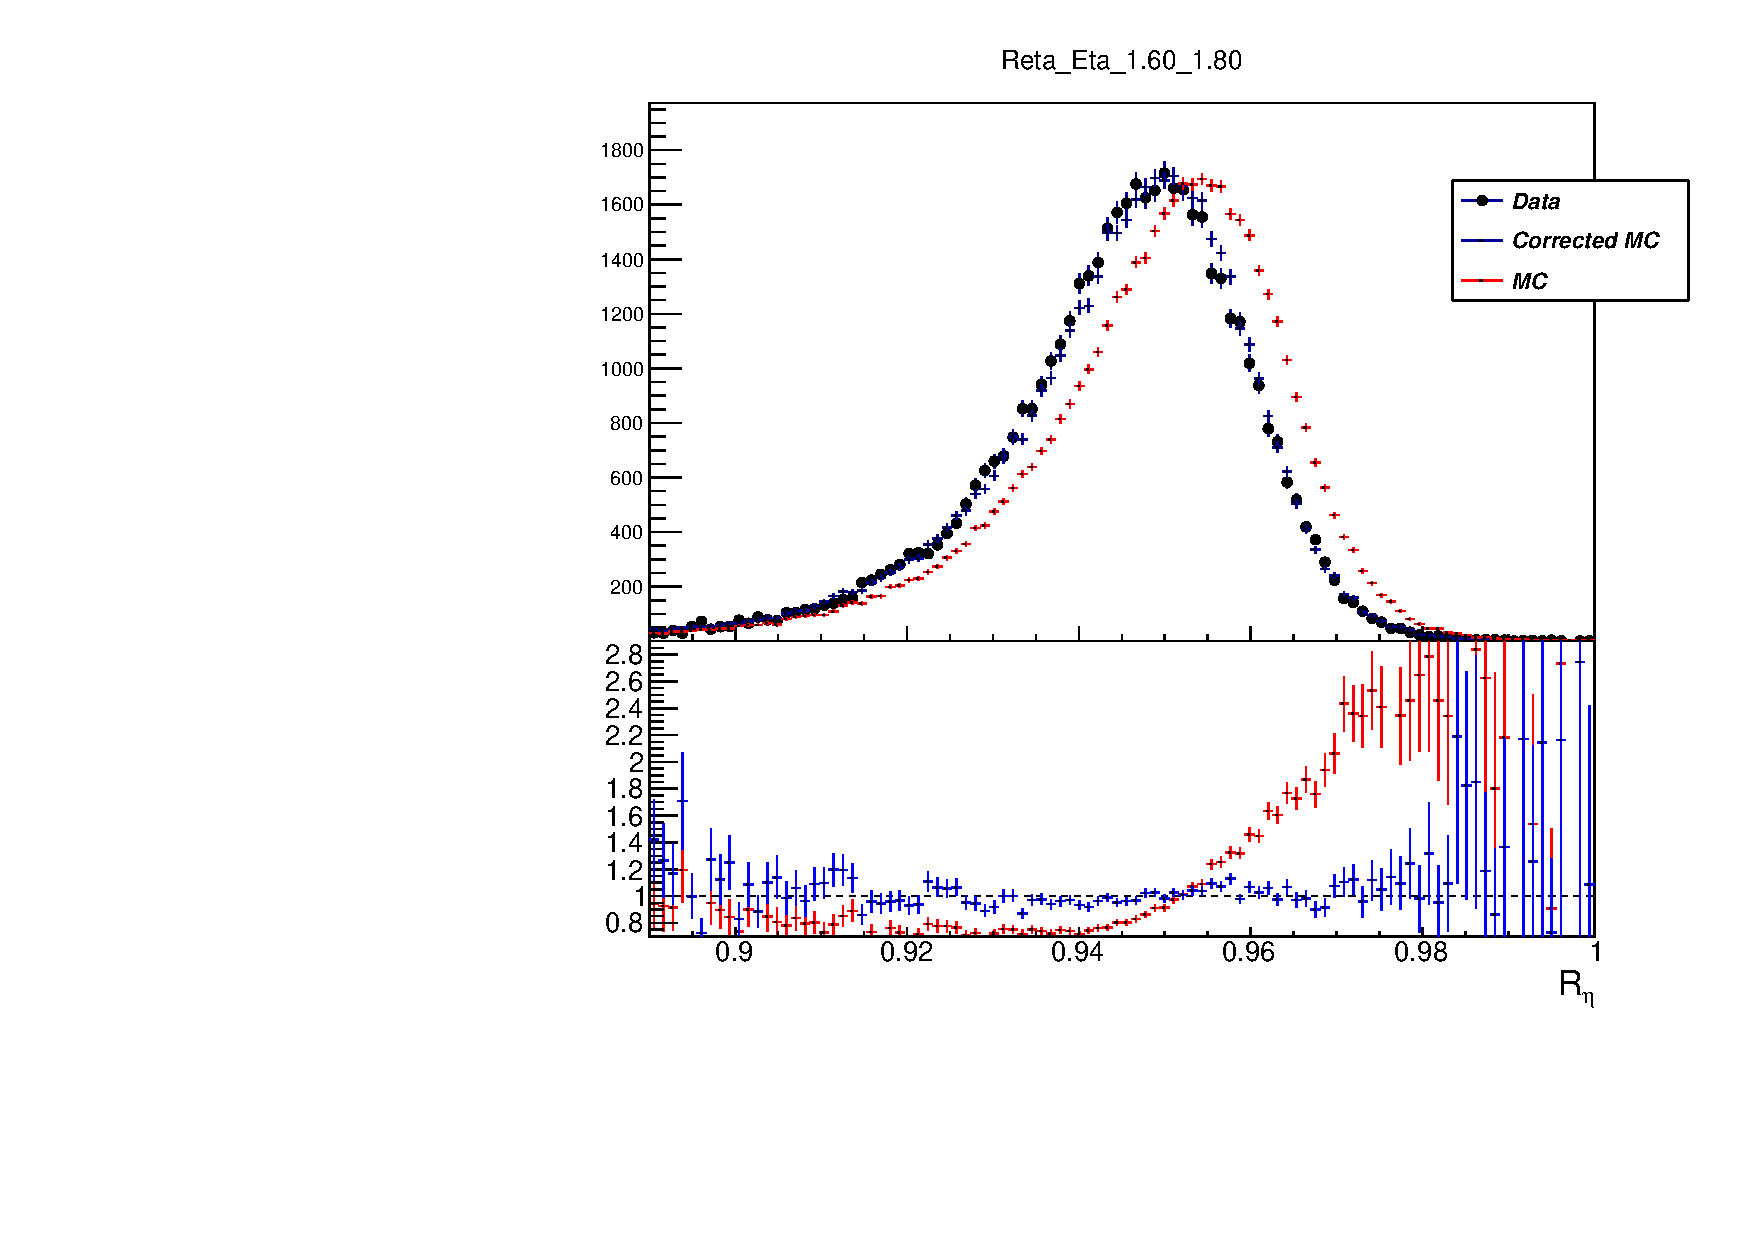
\includegraphics[width=0.33\textwidth]{Reta_Eta_16_18_Athena}}\\
	\quad
	\subfloat {%
		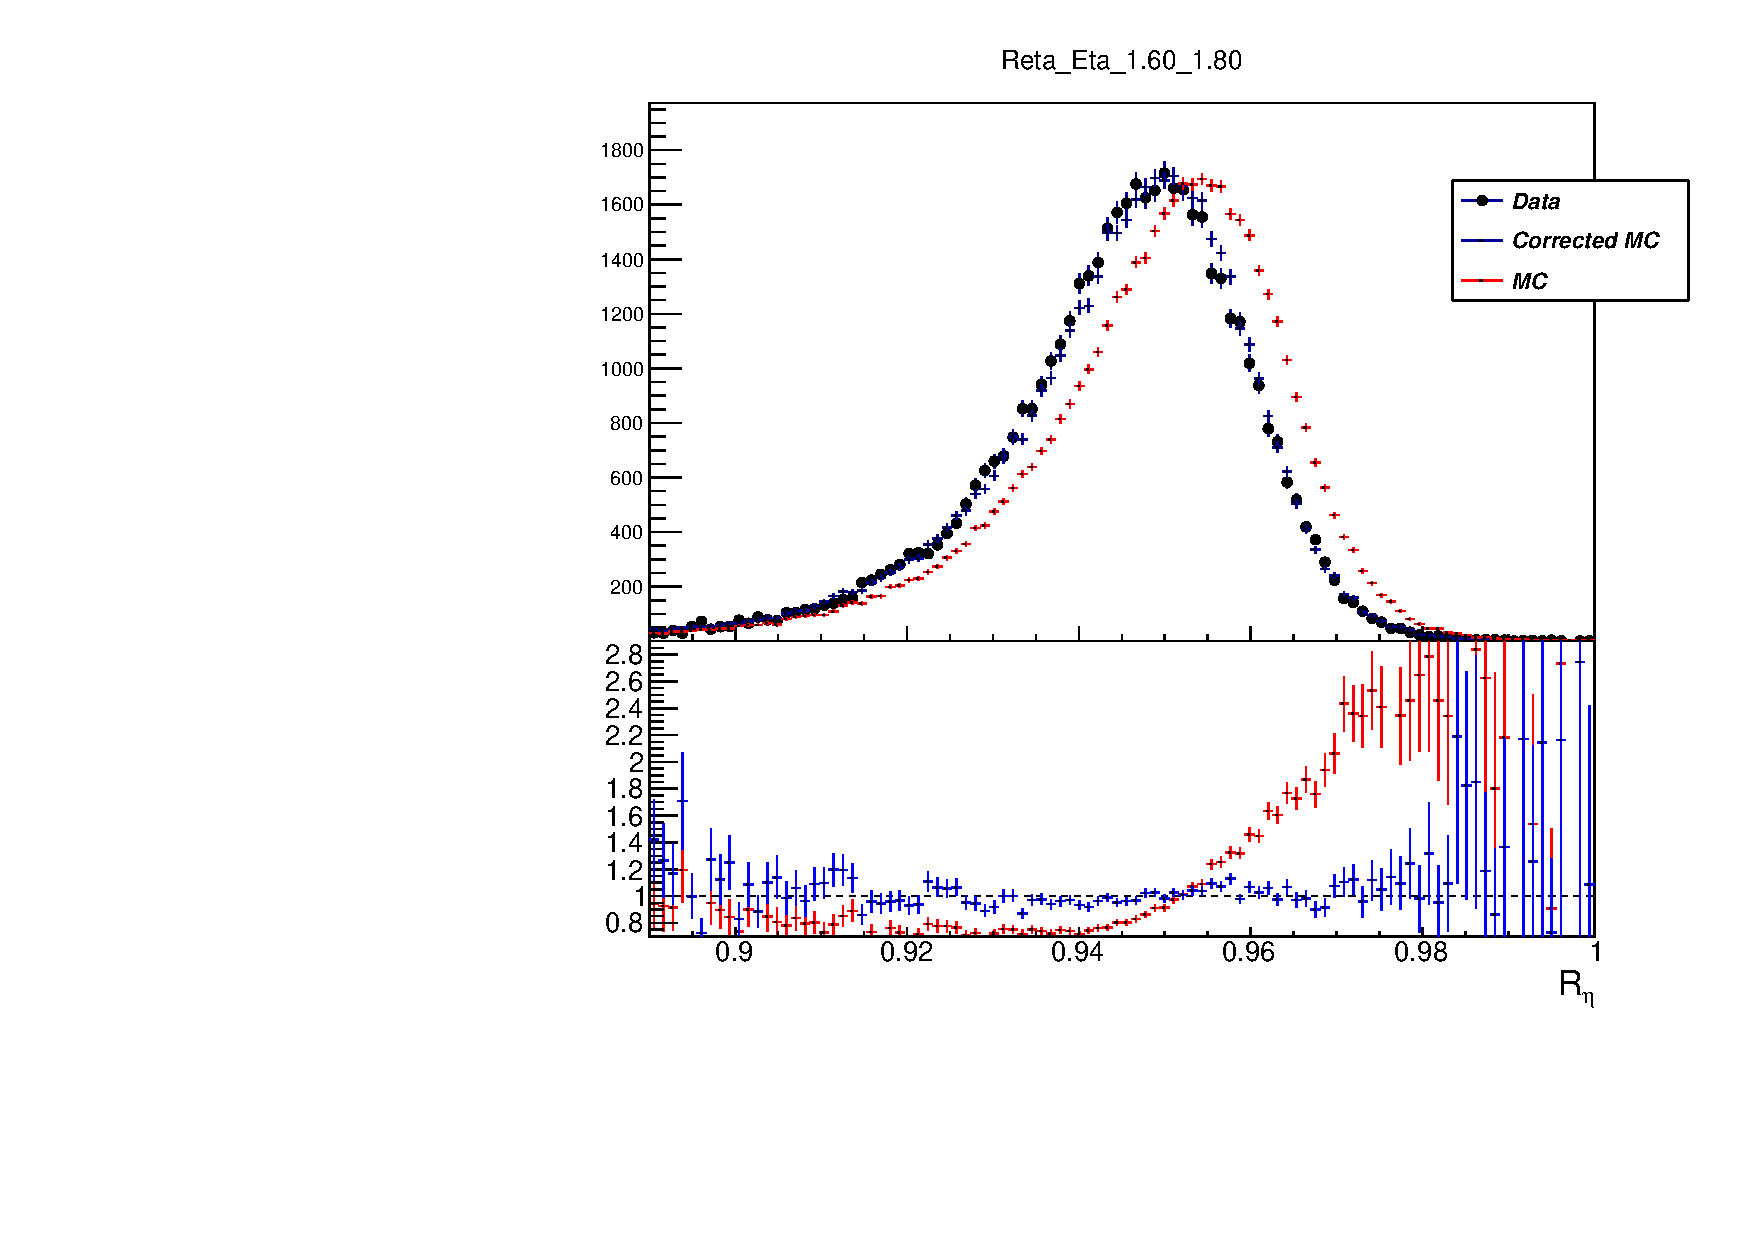
\includegraphics[width=0.33\textwidth]{Reta_Eta_16_18_Athena}}
	\quad
	\subfloat{%
		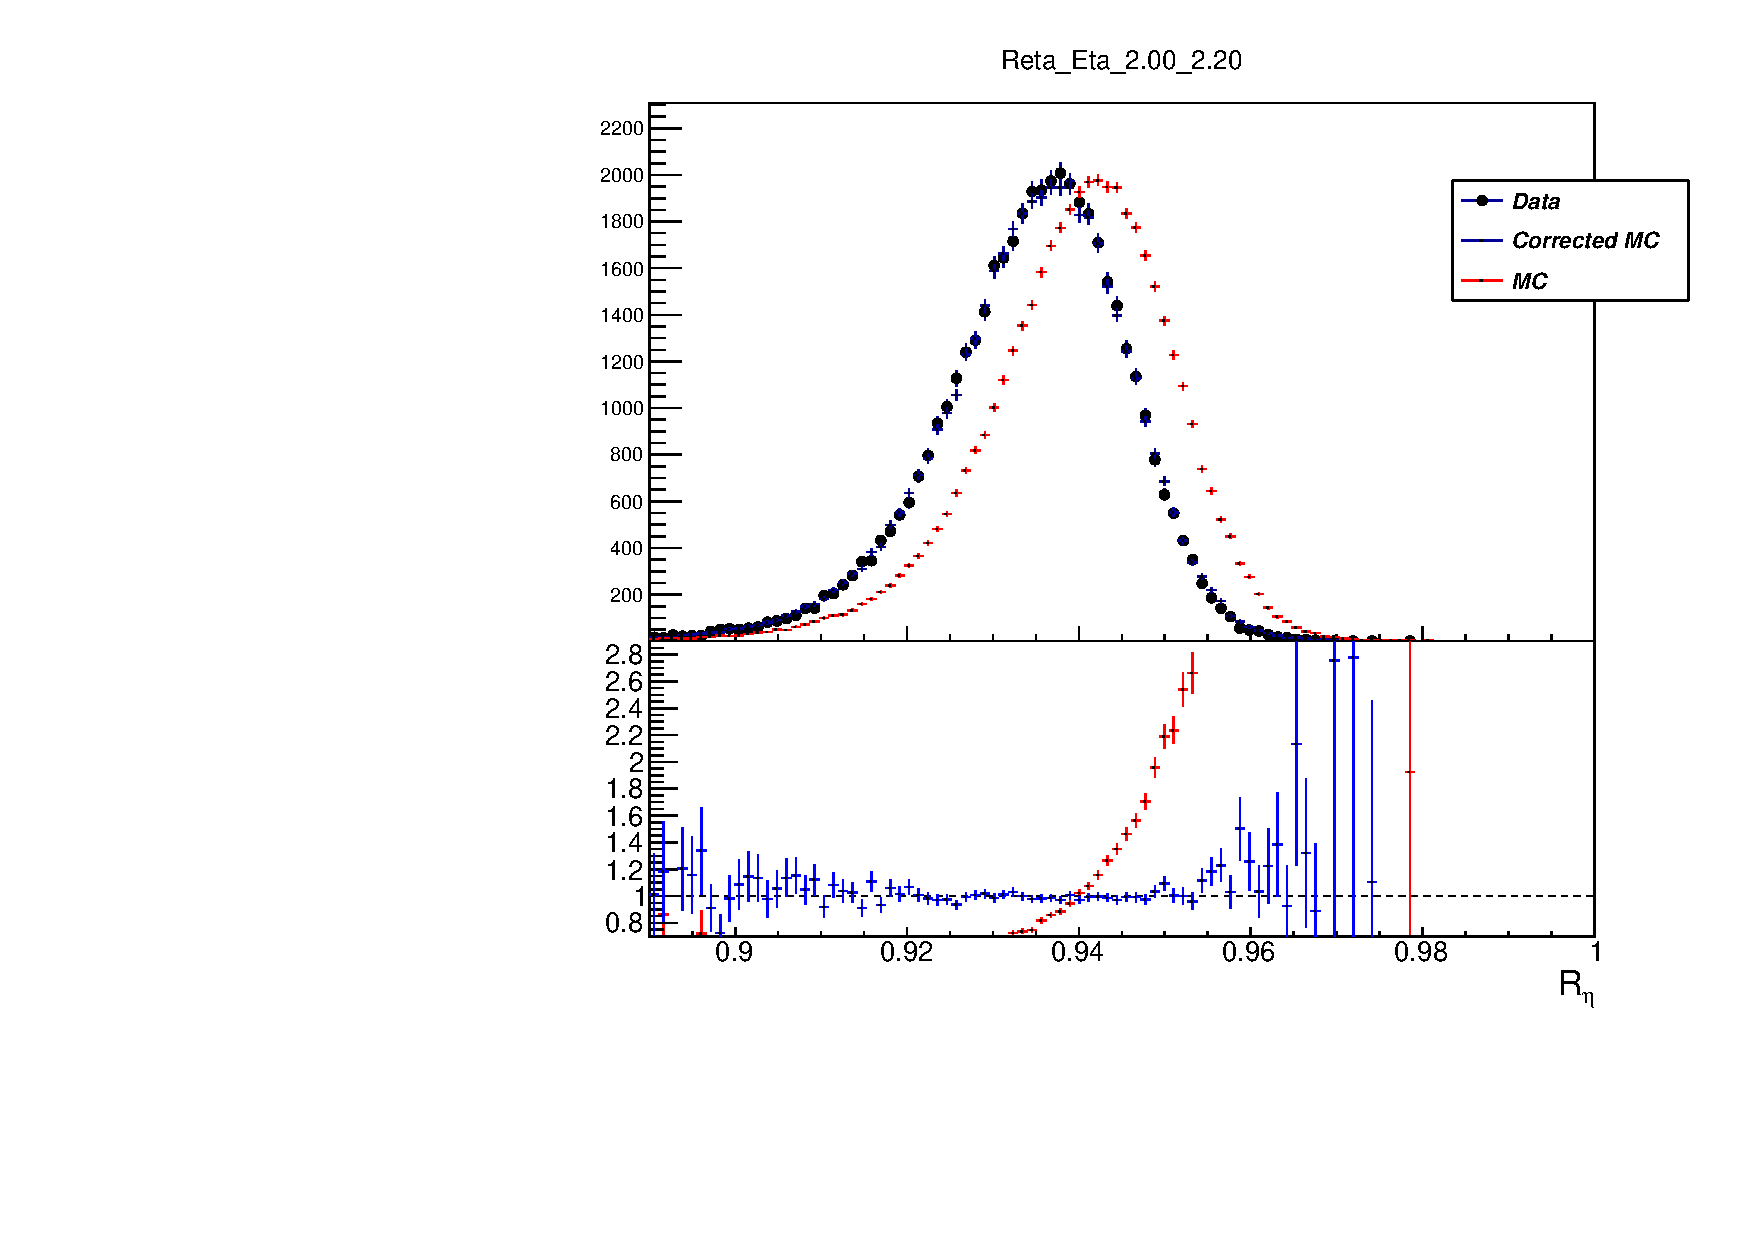
\includegraphics[width=0.33\textwidth]{Reta_Eta_20_22_Athena}}
		\quad
	\subfloat{%
		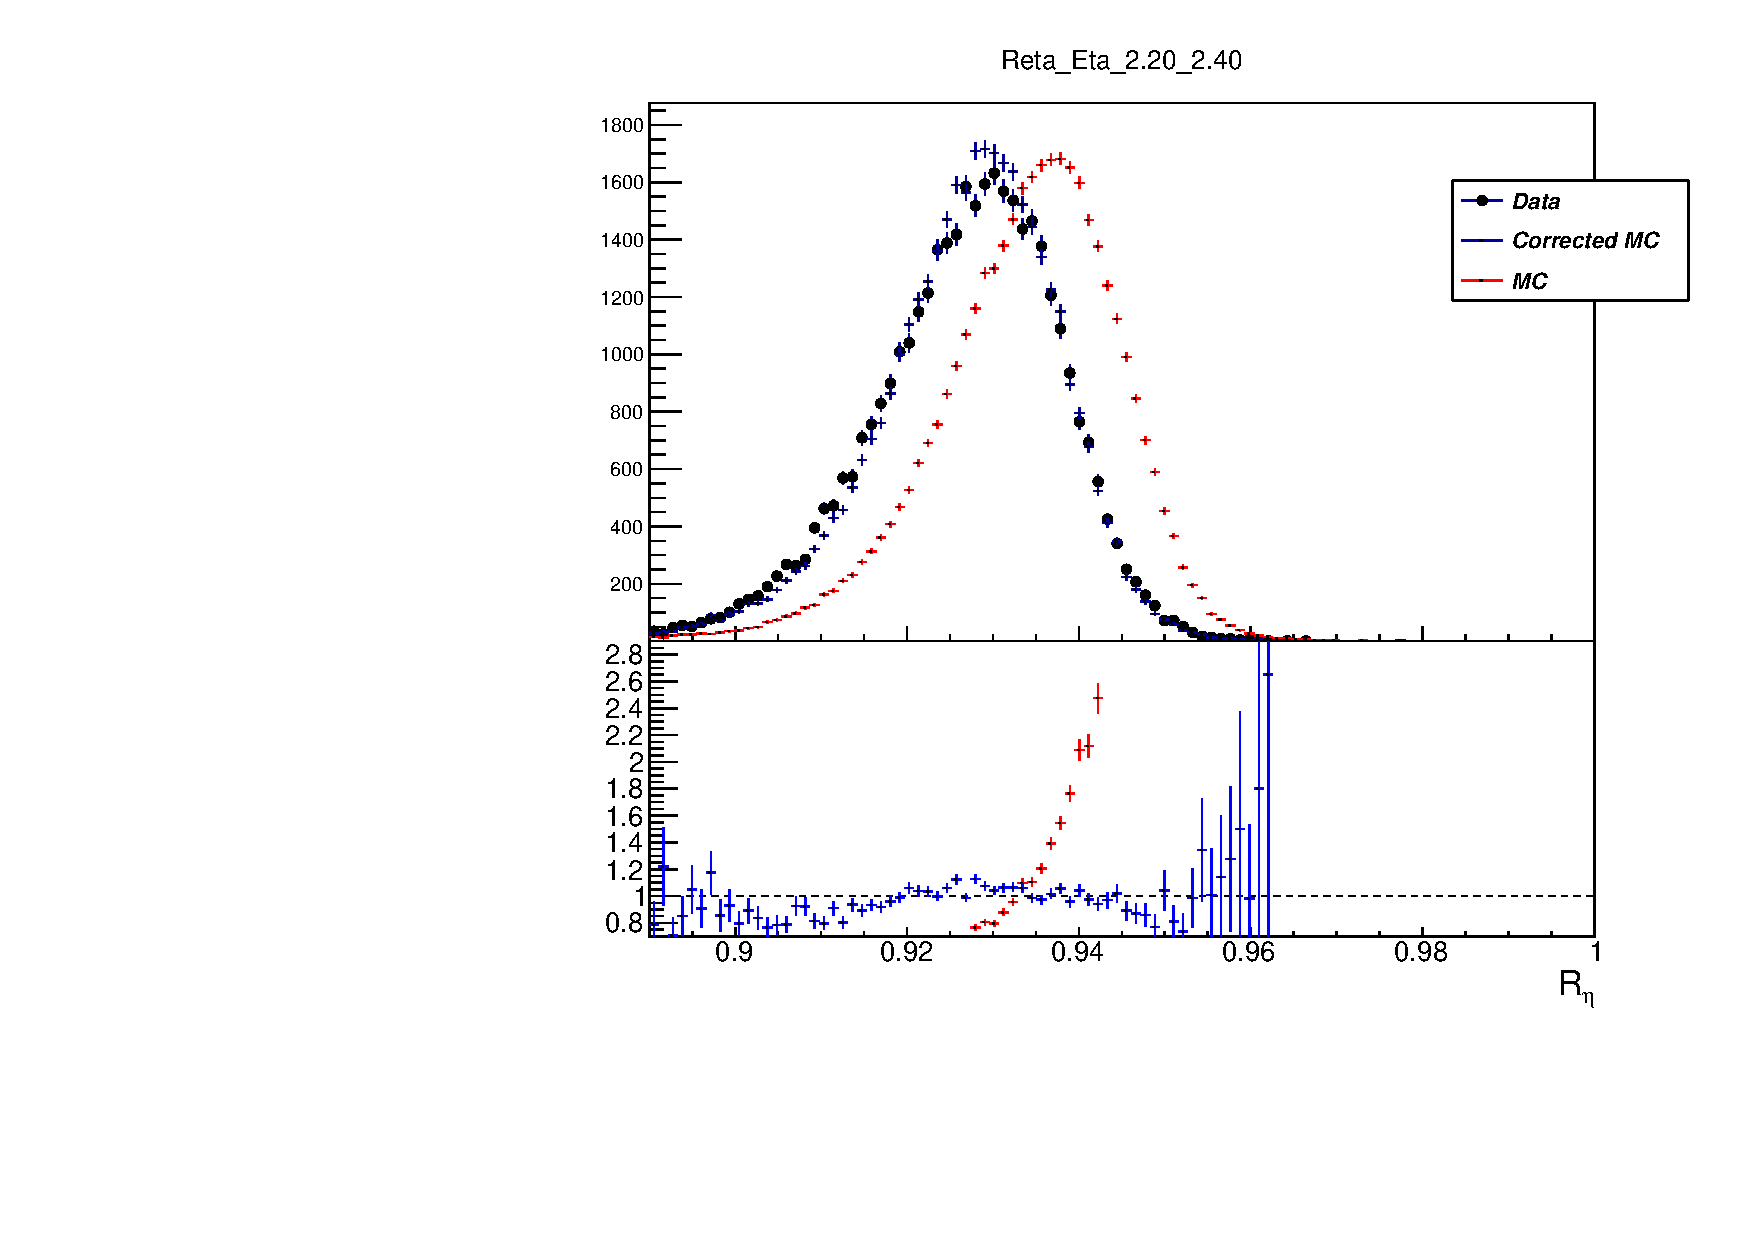
\includegraphics[width=0.33\textwidth]{Reta_Eta_22_24_Athena}}
	\caption{ 	\label{fig::reta_} $R_{\eta}$ in all eta slices.}
\end{figure*}

  \begin{figure*}[ht!]
	\subfloat{%
		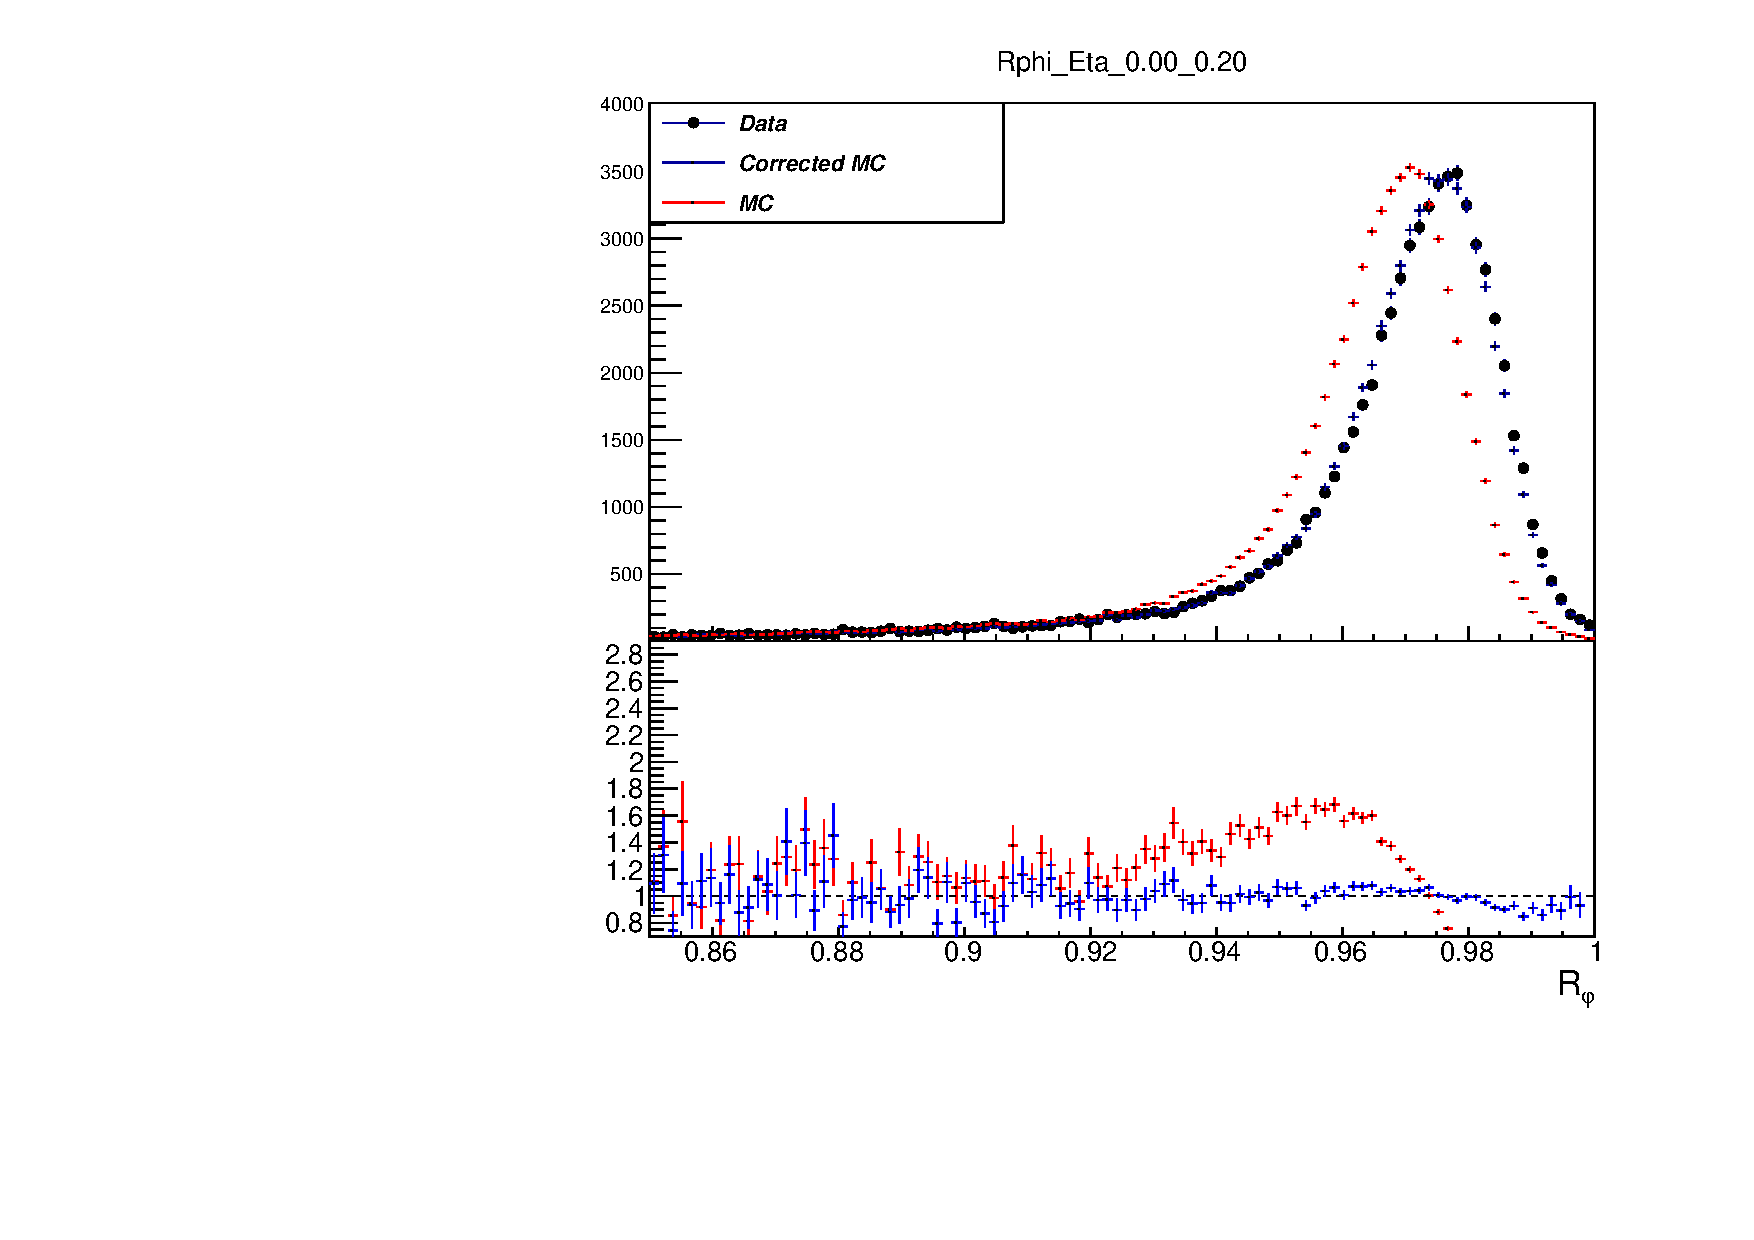
\includegraphics[width=0.33\textwidth]{Rphi_Eta_0_2_Athena}}
	\quad
	\subfloat {%
		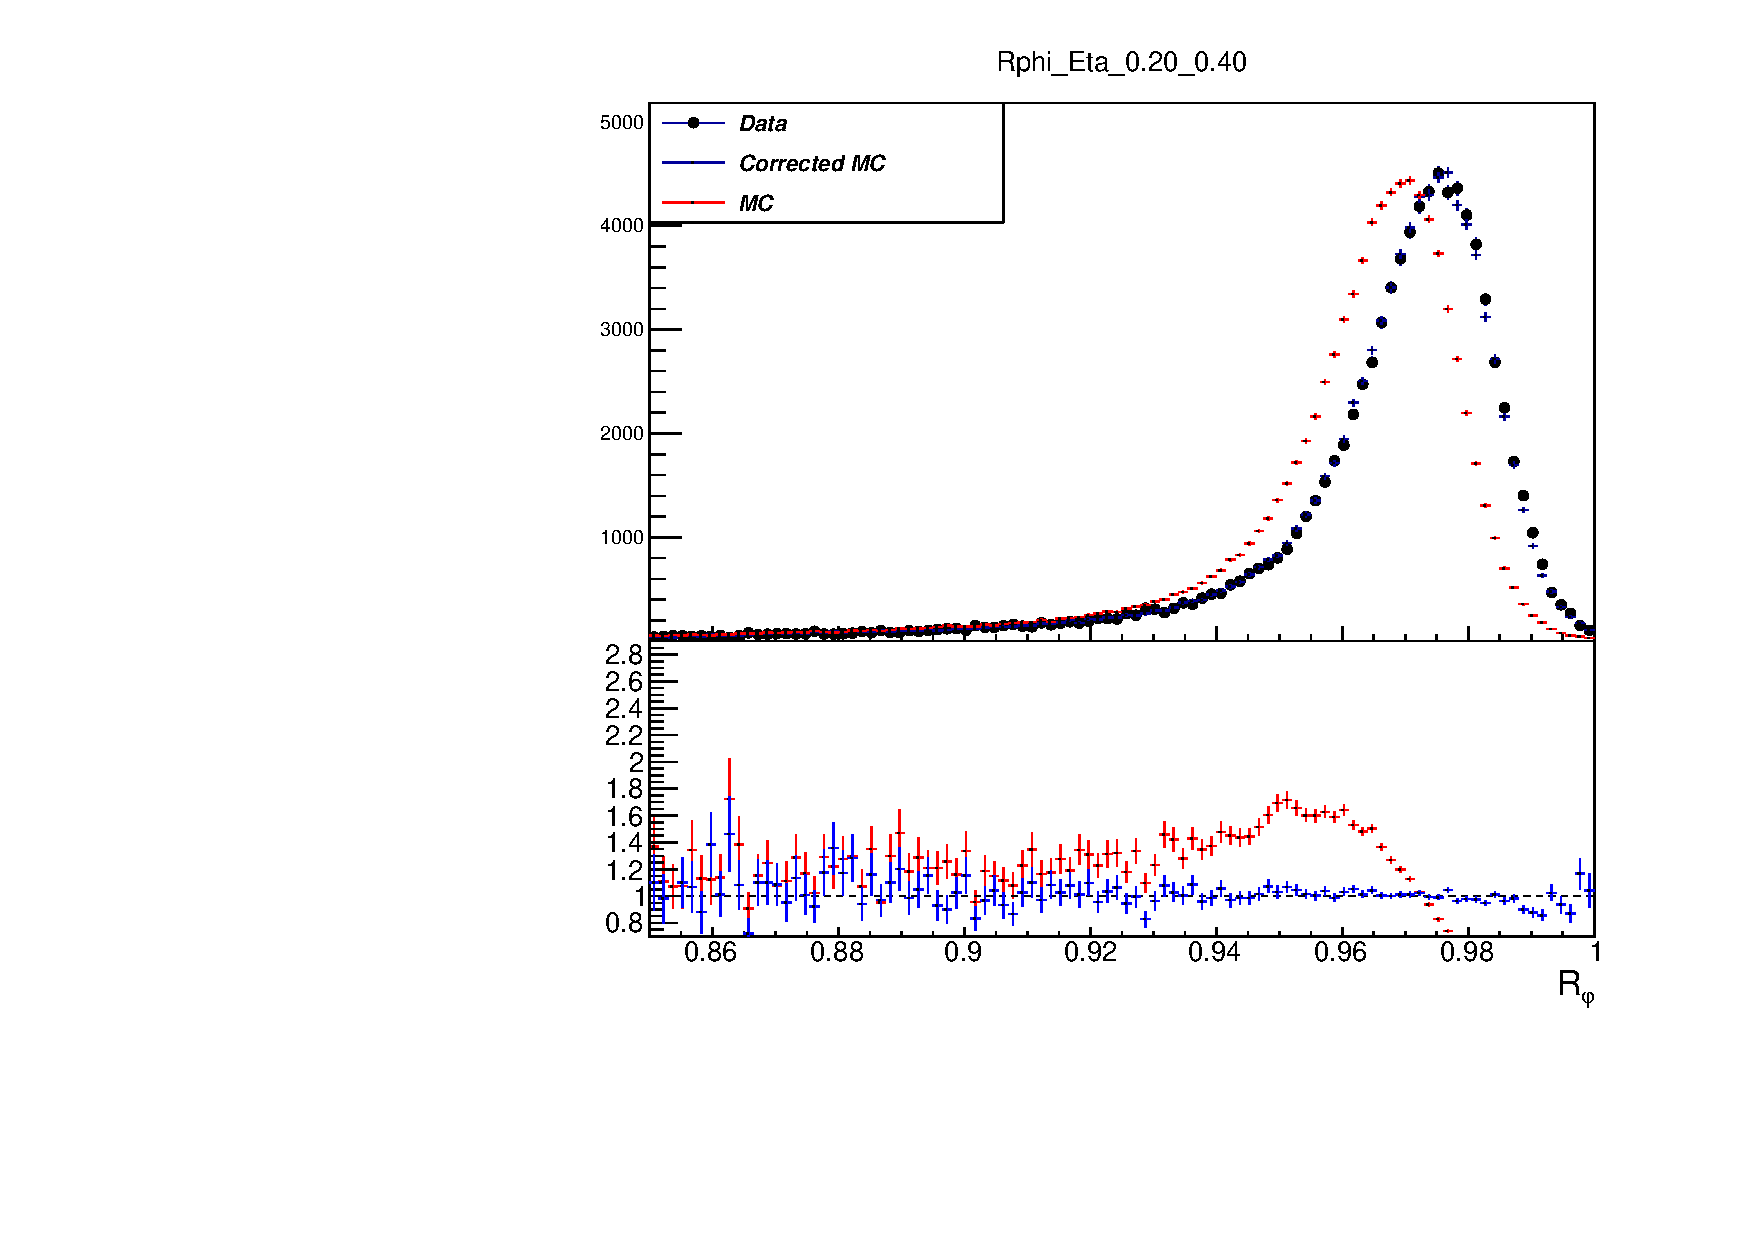
\includegraphics[width=0.33\textwidth]{Rphi_Eta_2_4_Athena}}
	\quad
	\subfloat{%
		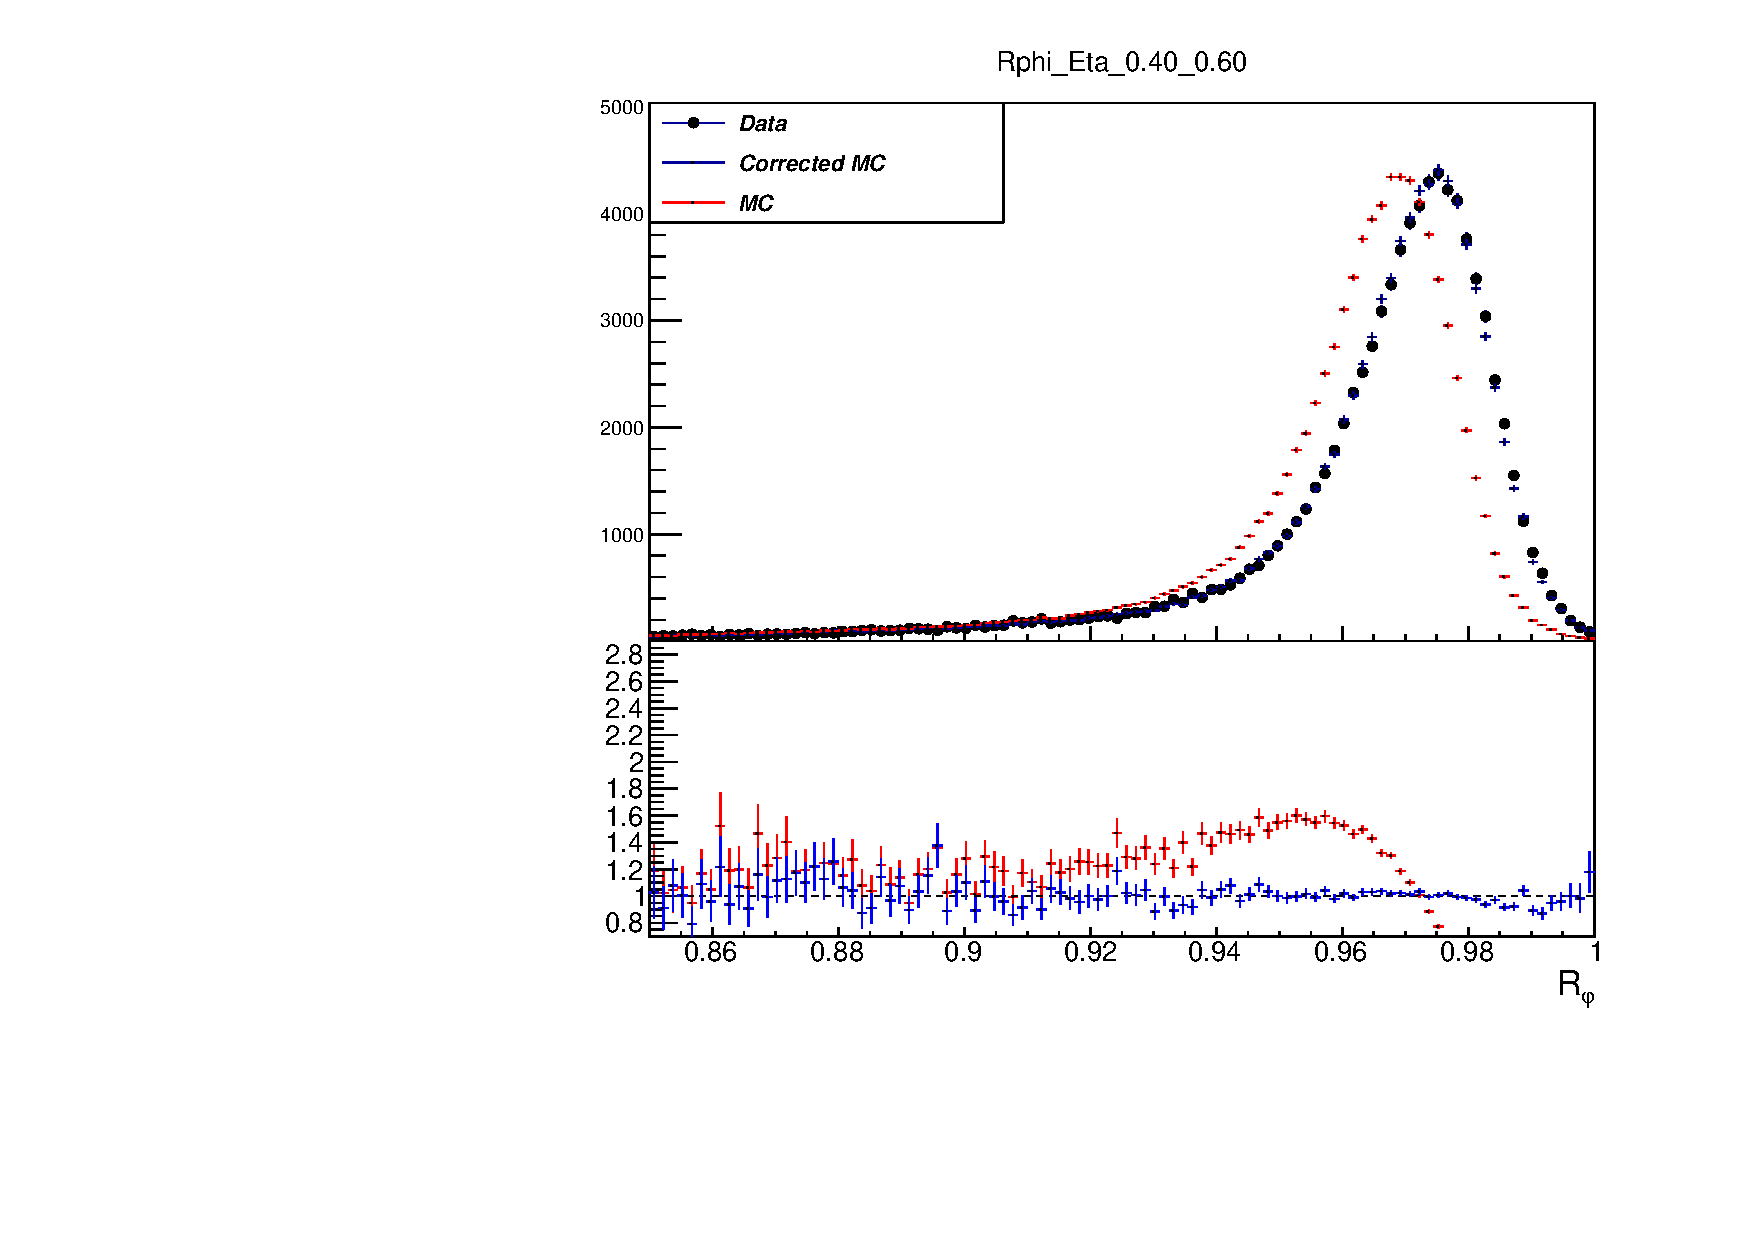
\includegraphics[width=0.33\textwidth]{Rphi_Eta_4_6_Athena}}\\
	\subfloat{%
		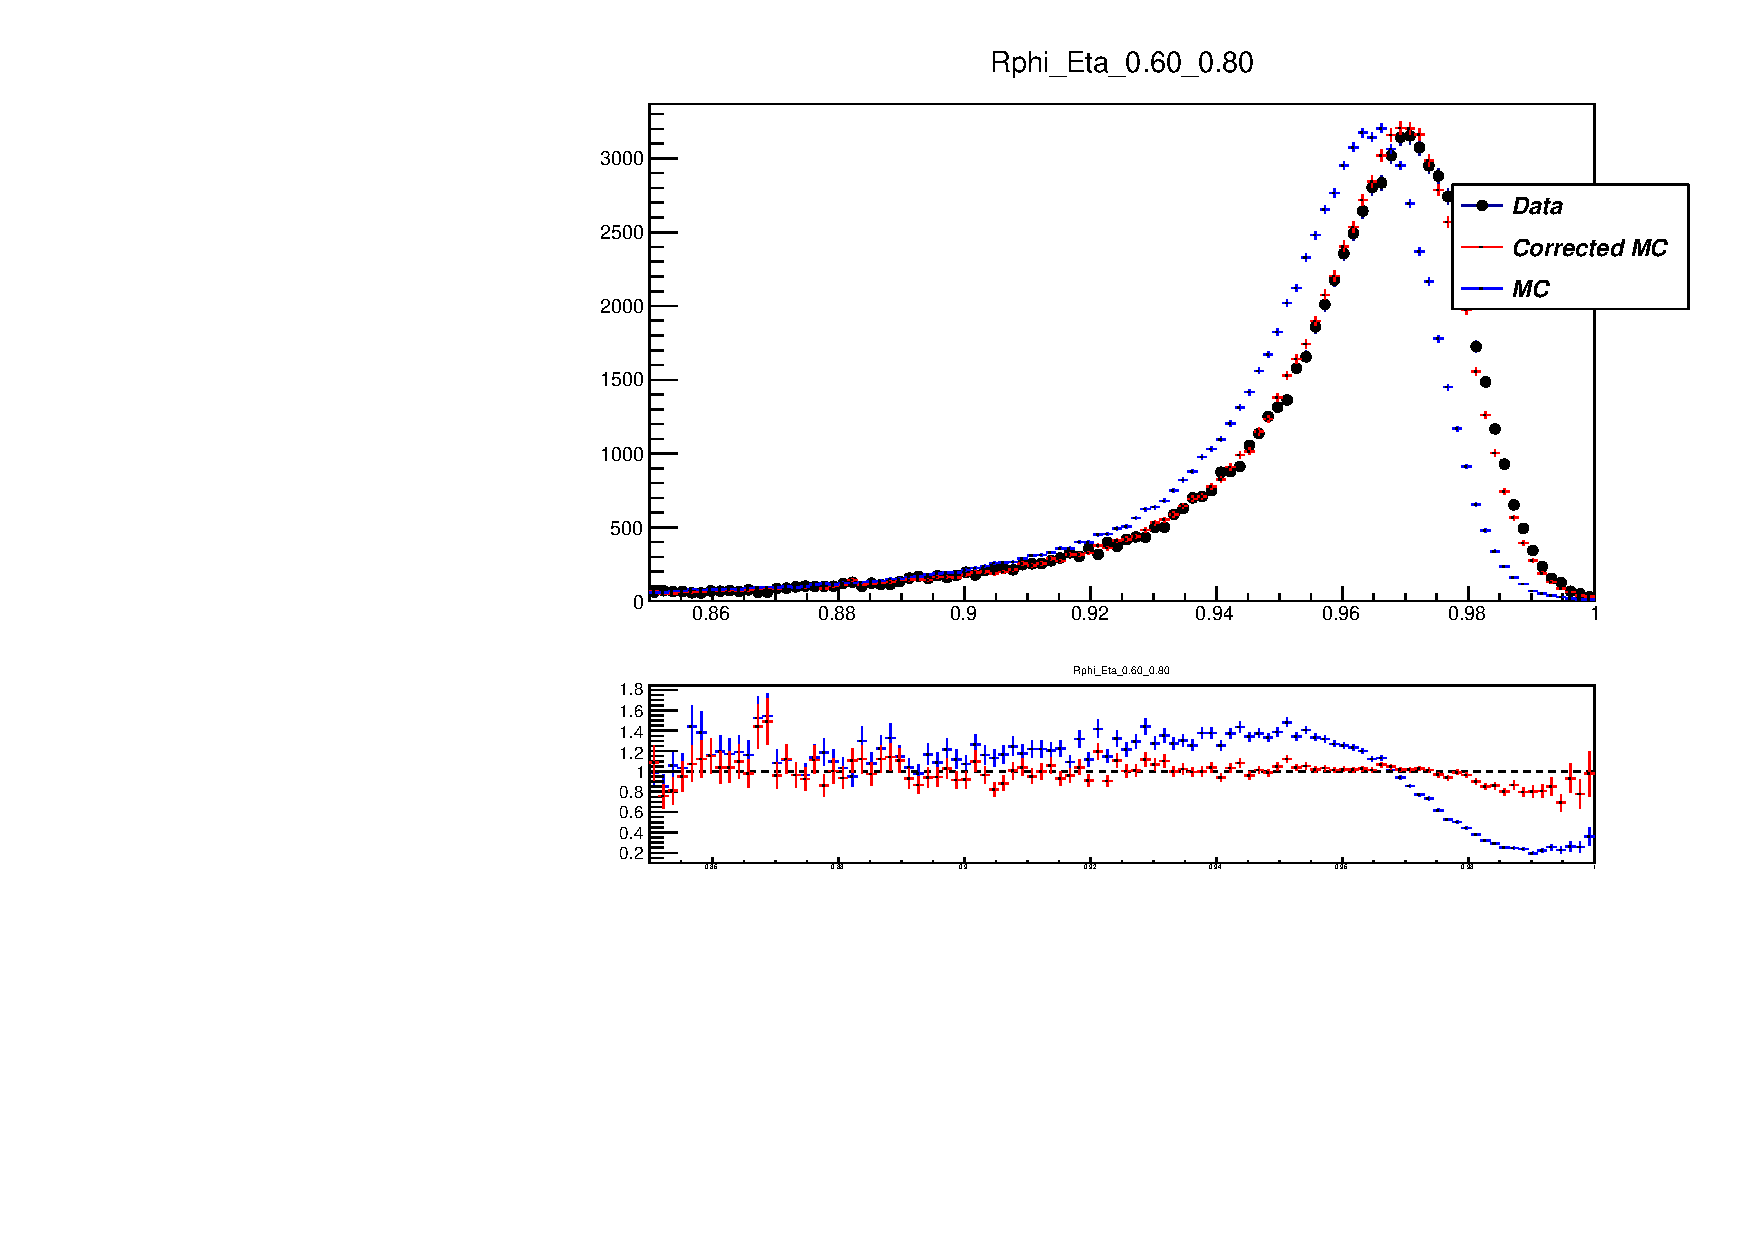
\includegraphics[width=0.33\textwidth]{Rphi_Eta_6_8_Athena}}
	\quad
	\subfloat {%
		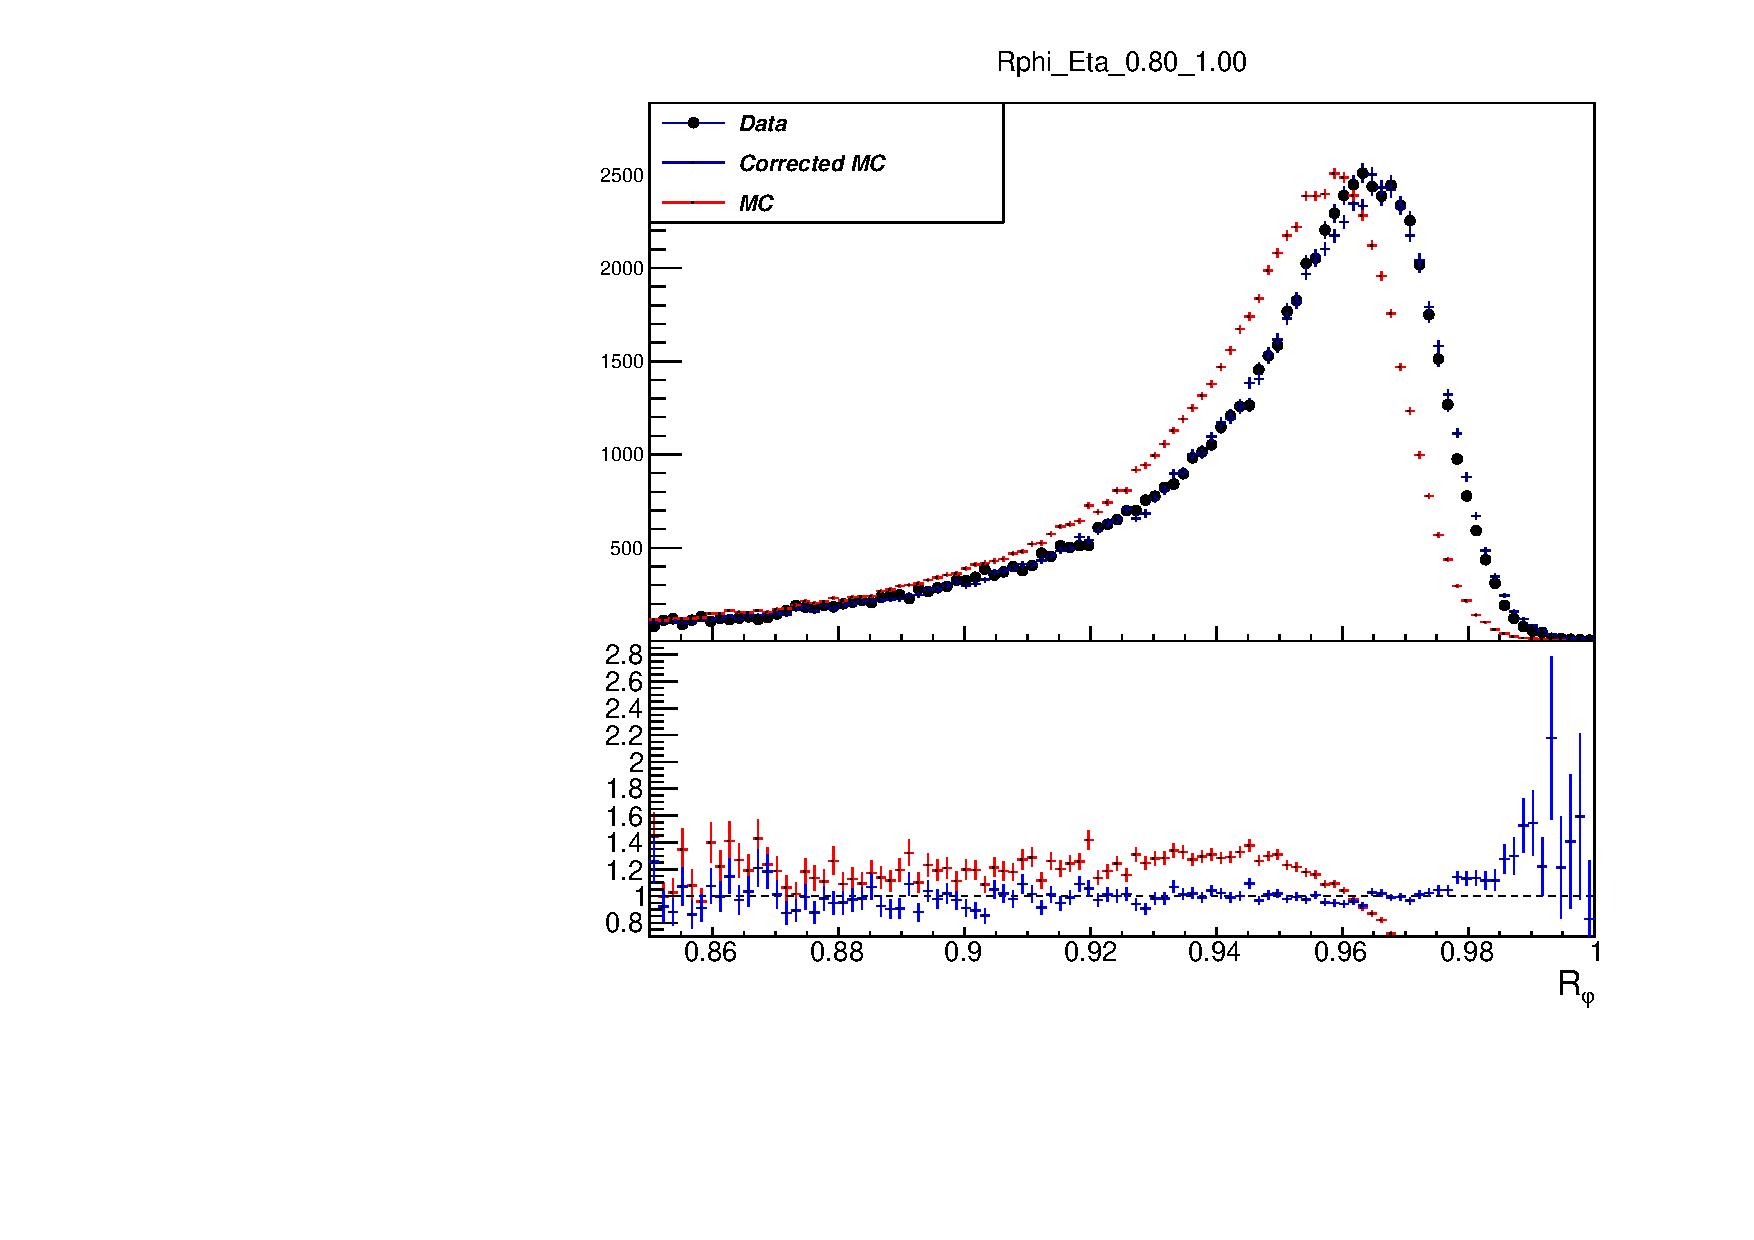
\includegraphics[width=0.33\textwidth]{Rphi_Eta_8_10_Athena}}
	\quad
	\subfloat{%
		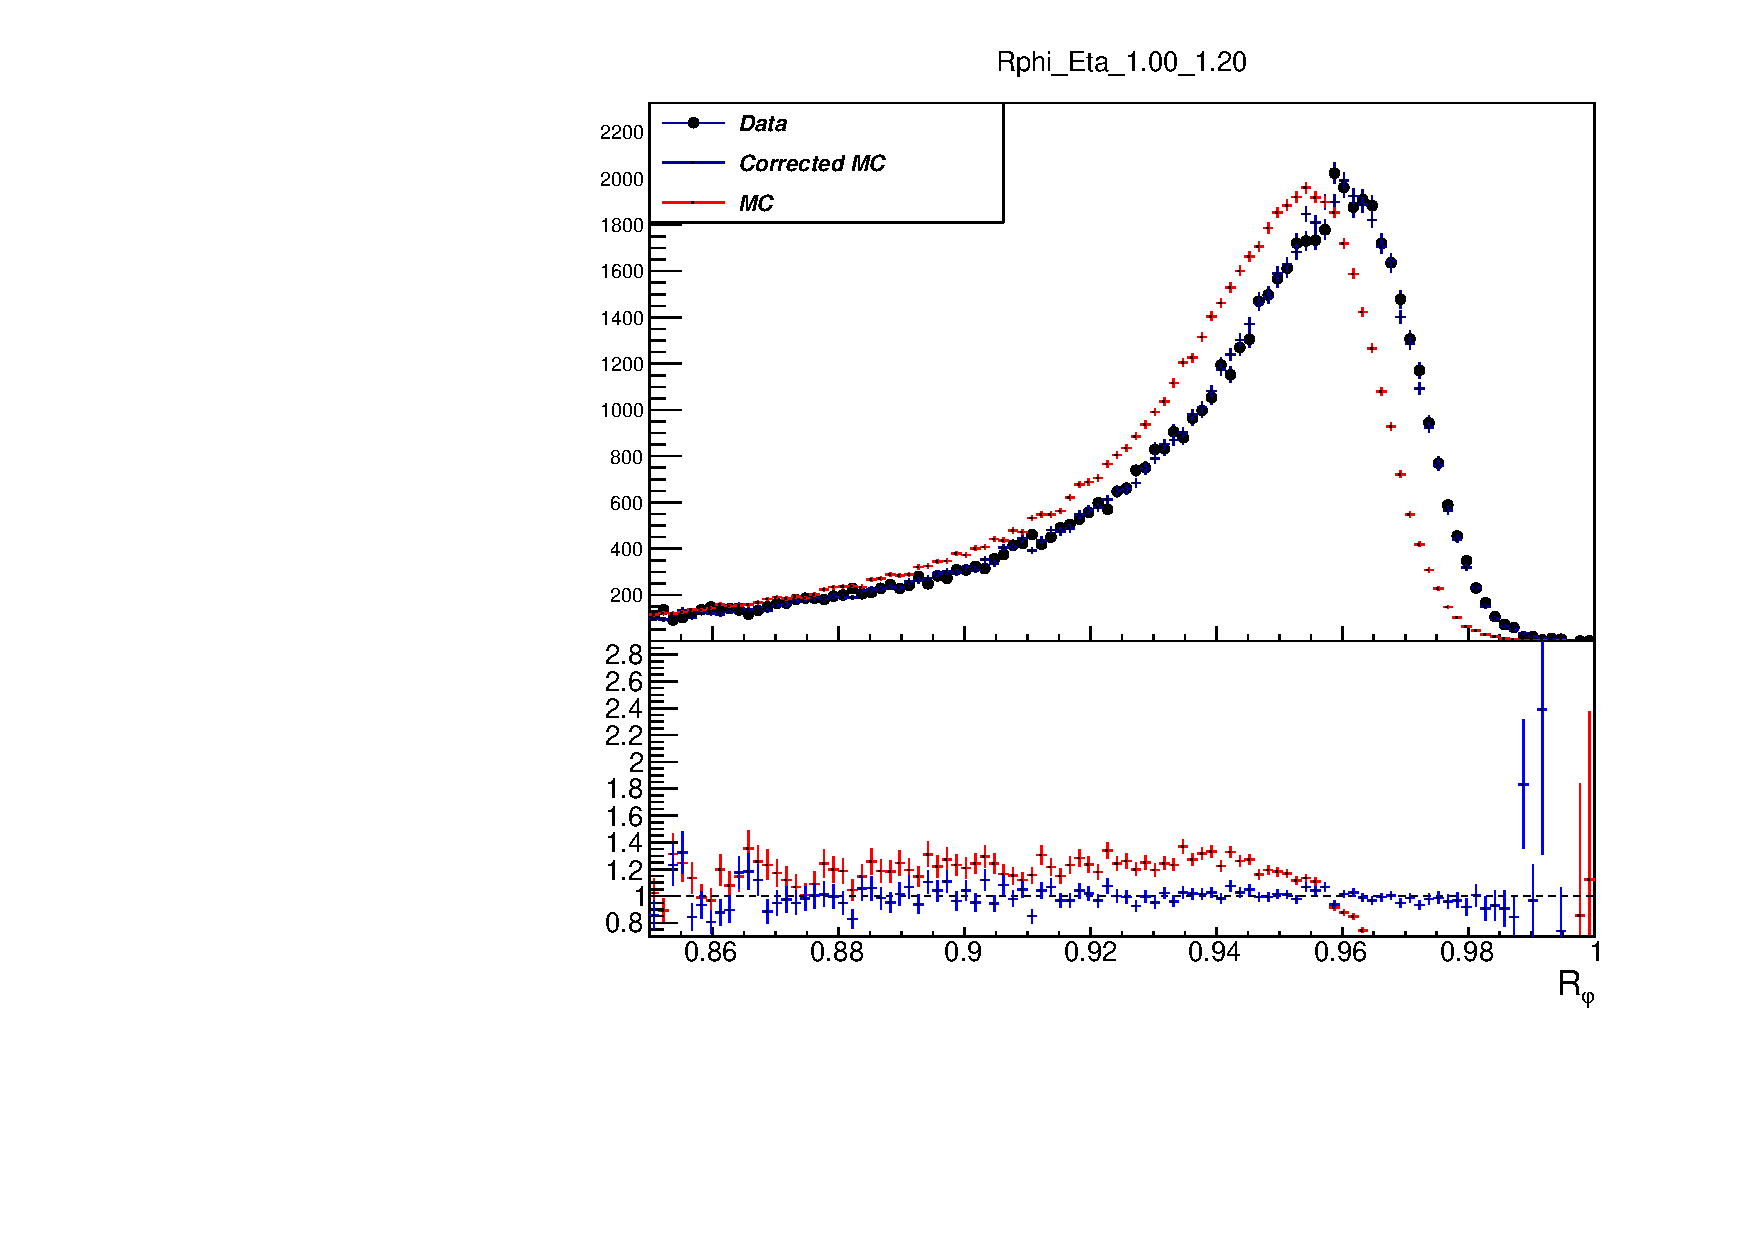
\includegraphics[width=0.33\textwidth]{Rphi_Eta_10_12_Athena}}\\
	\subfloat{%
		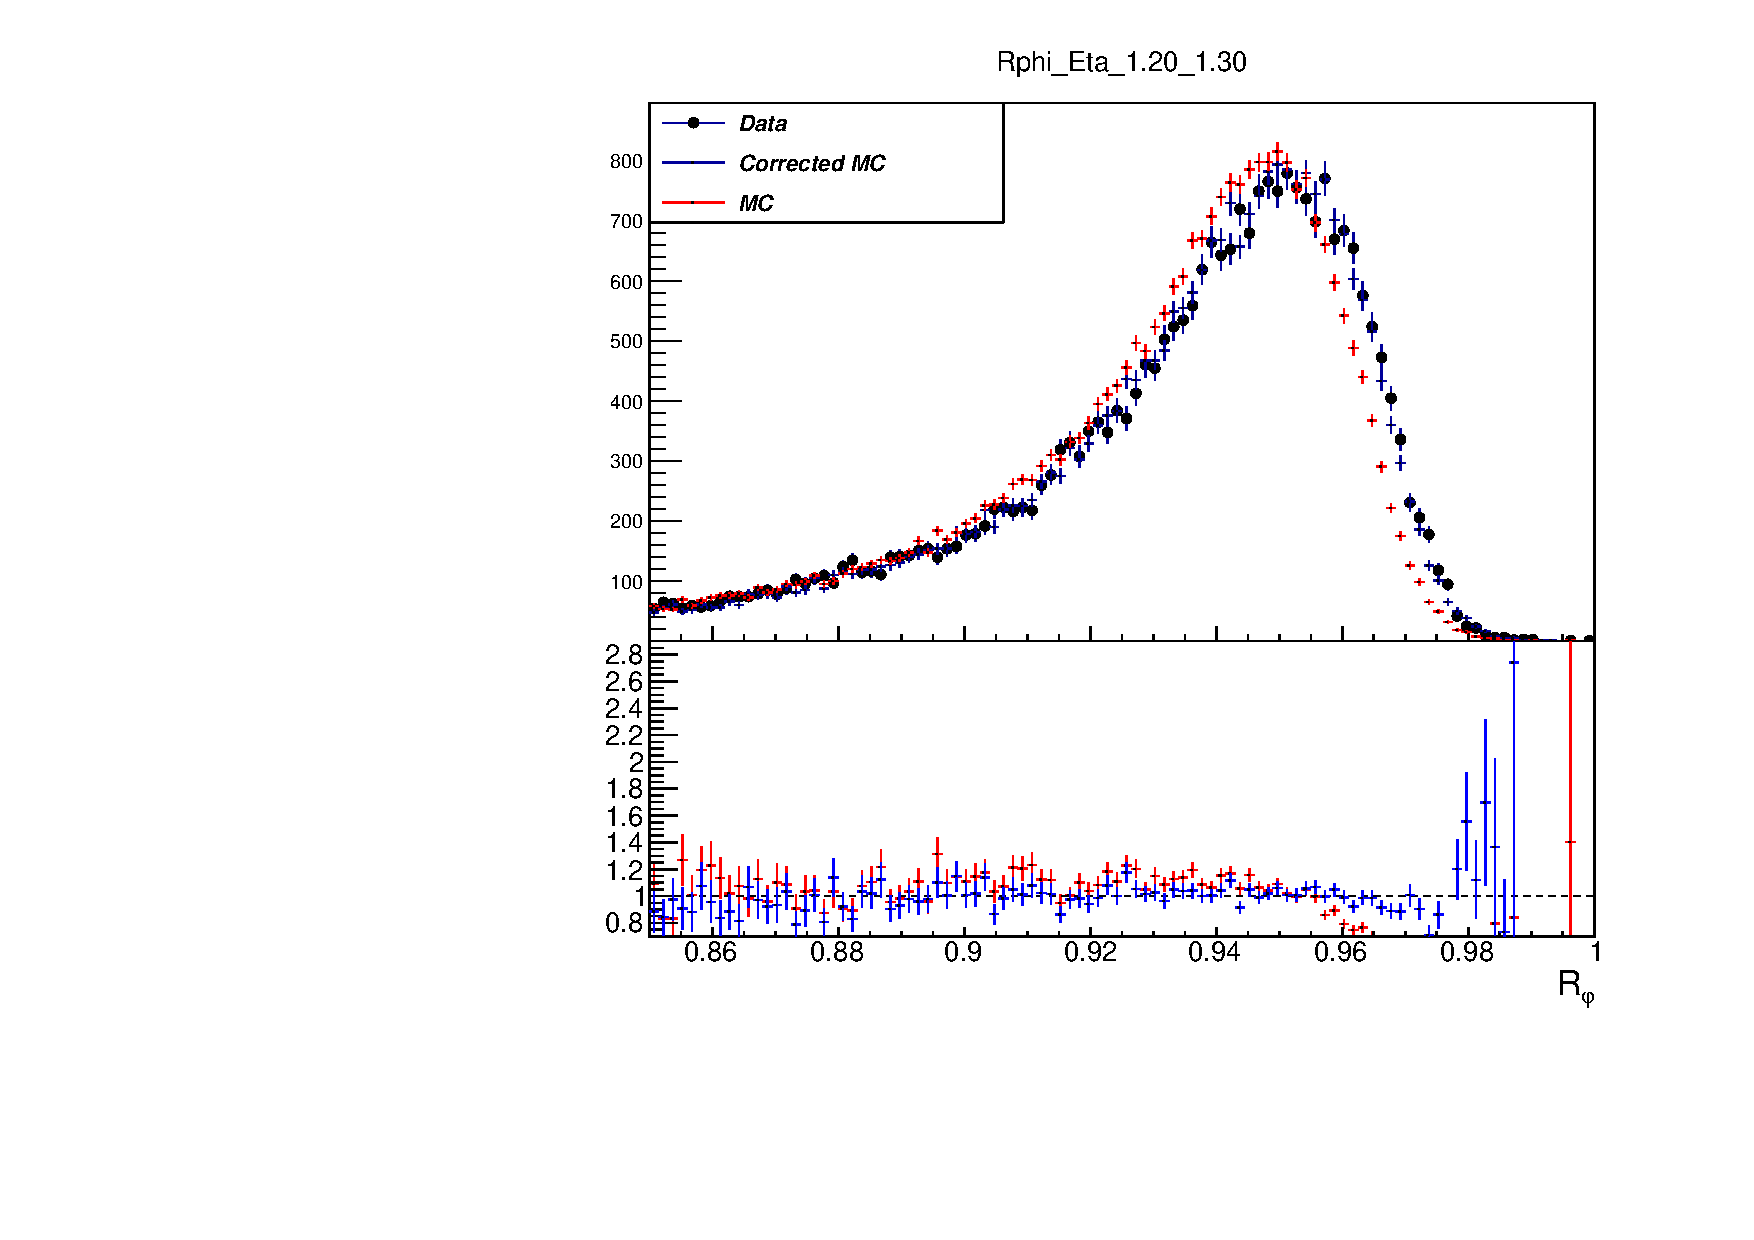
\includegraphics[width=0.33\textwidth]{Rphi_Eta_12_13_Athena}}
	\quad
	\subfloat{%
		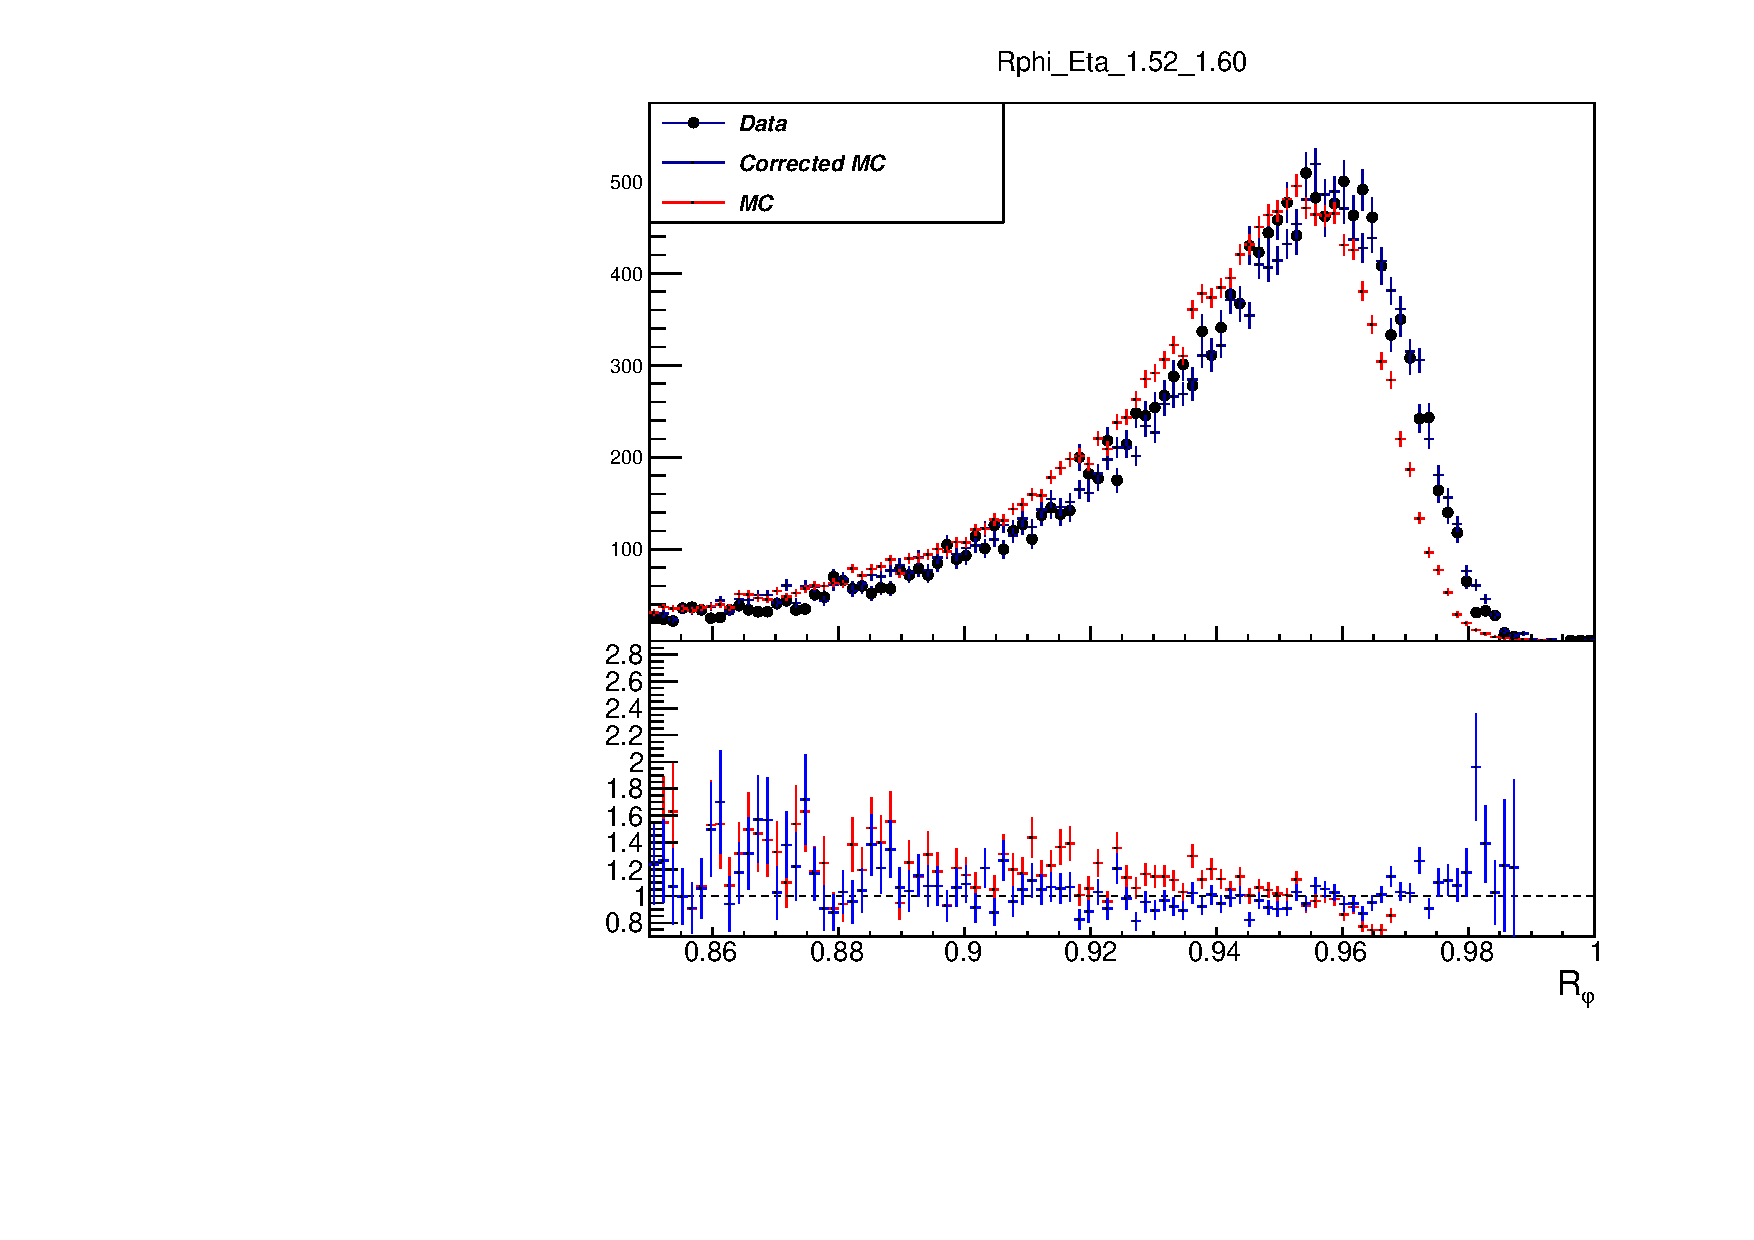
\includegraphics[width=0.33\textwidth]{Rphi_Eta_152_16_Athena}}
	\subfloat{%
		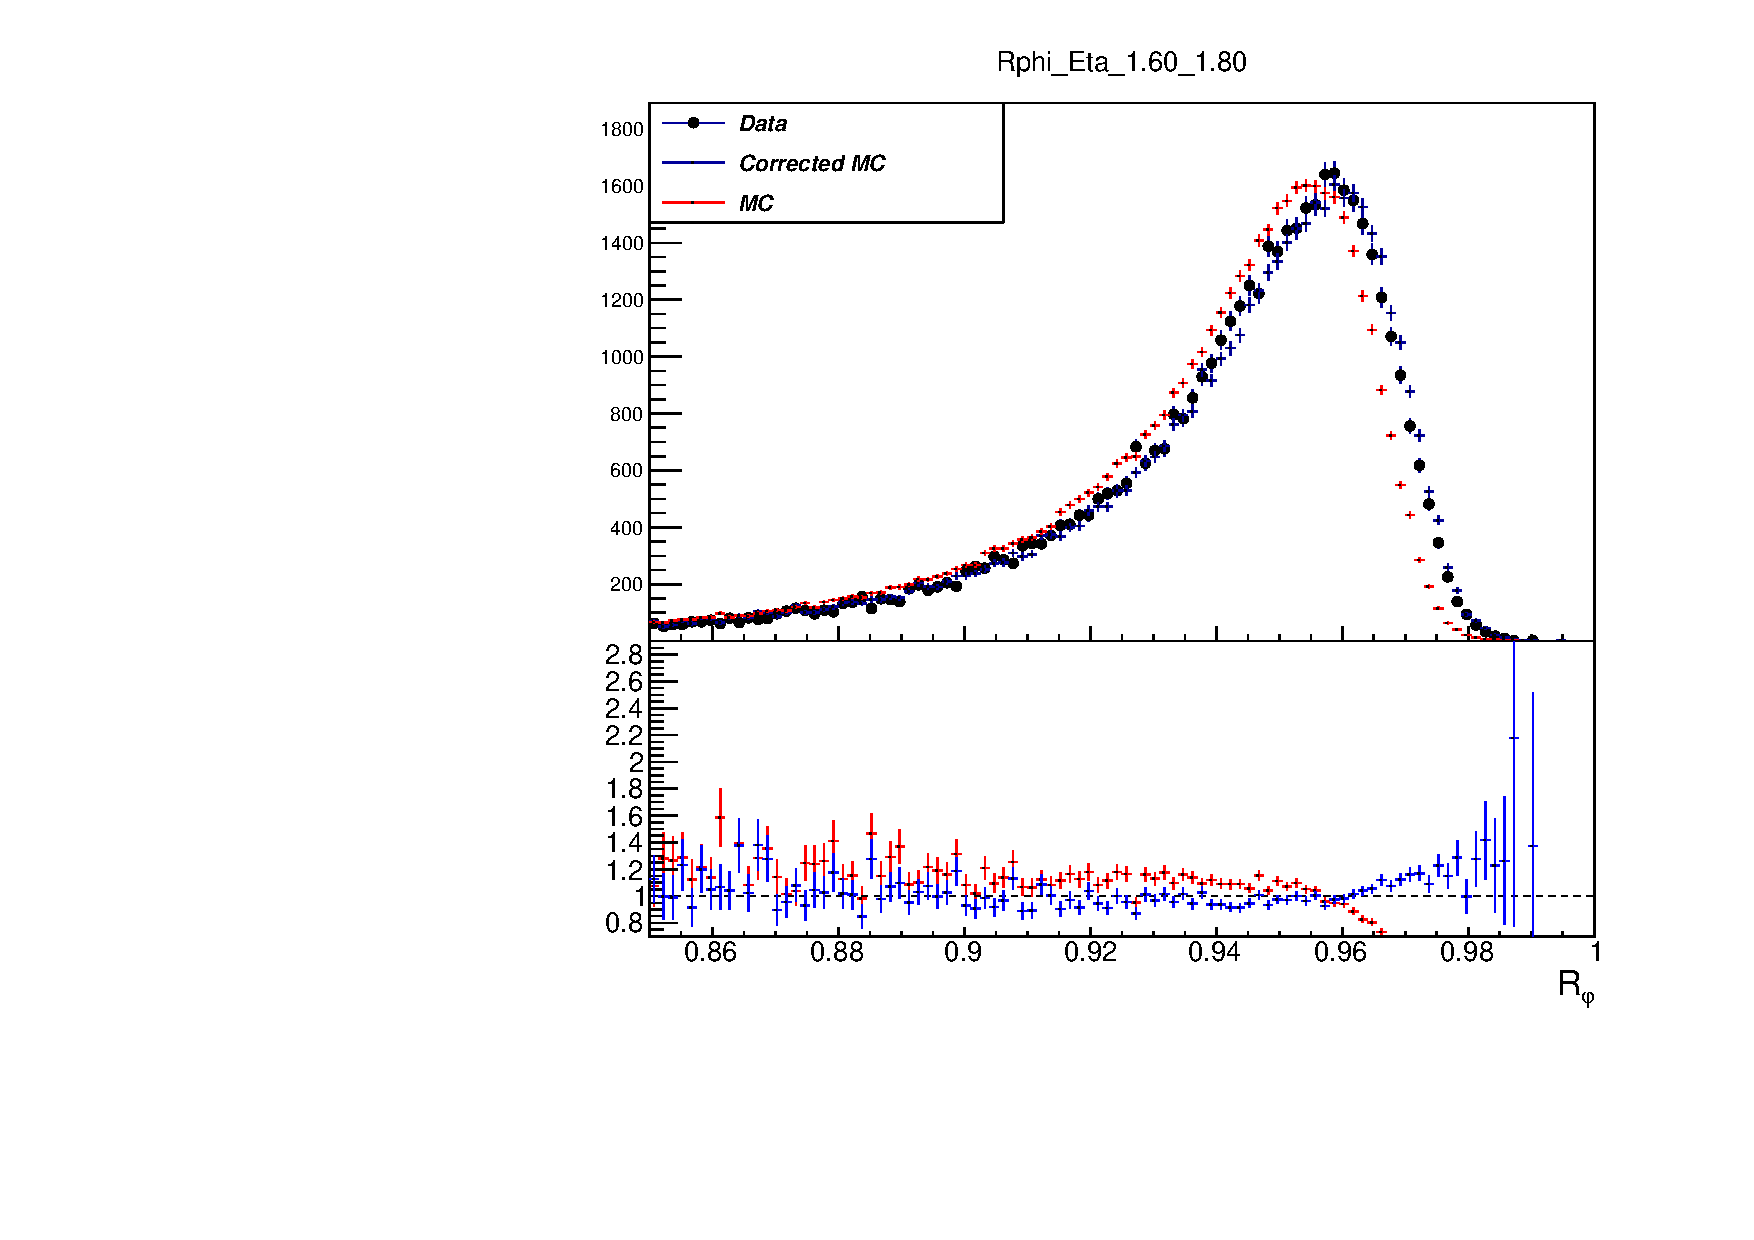
\includegraphics[width=0.33\textwidth]{Rphi_Eta_16_18_Athena}}\\
	\quad
	\subfloat {%
		\includegraphics[width=0.33\textwidth]{Rphi_Eta_16_18_Athena}}
	\quad
	\subfloat{%
		\includegraphics[width=0.33\textwidth]{Rphi_Eta_20_22_Athena}}
	\quad
	\subfloat{%
		\includegraphics[width=0.33\textwidth]{Rphi_Eta_22_24_Athena}}
	\caption{ 	\label{fig::rphi_} $R_{\phi}$ in all eta slices.}
\end{figure*}

  \begin{figure*}[ht!]
	\subfloat{%
		\includegraphics[width=0.33\textwidth]{Weta2_Eta_0_2_Athena}}
	\quad
	\subfloat {%
		\includegraphics[width=0.33\textwidth]{Weta2_Eta_2_4_Athena}}
	\quad
	\subfloat{%
		\includegraphics[width=0.33\textwidth]{Weta2_Eta_4_6_Athena}}\\
	\subfloat{%
		\includegraphics[width=0.33\textwidth]{Weta2_Eta_6_8_Athena}}
	\quad
	\subfloat {%
		\includegraphics[width=0.33\textwidth]{Weta2_Eta_8_10_Athena}}
	\quad
	\subfloat{%
		\includegraphics[width=0.33\textwidth]{Weta2_Eta_10_12_Athena}}\\
	\subfloat{%
		\includegraphics[width=0.33\textwidth]{Weta2_Eta_12_13_Athena}}
	\quad
	\subfloat{%
		\includegraphics[width=0.33\textwidth]{Weta2_Eta_152_16_Athena}}
	\subfloat{%
		\includegraphics[width=0.33\textwidth]{Weta2_Eta_16_18_Athena}}\\
	\quad
	\subfloat {%
		\includegraphics[width=0.33\textwidth]{Weta2_Eta_16_18_Athena}}
	\quad
	\subfloat{%
		\includegraphics[width=0.33\textwidth]{Weta2_Eta_20_22_Athena}}
	\quad
	\subfloat{%
		\includegraphics[width=0.33\textwidth]{Weta2_Eta_22_24_Athena}}
	\caption{ 	\label{fig::weta2_2} $W_{\eta2}$in all eta slices.}
\end{figure*}


  \begin{figure*}[ht!]
	\subfloat{%
		\includegraphics[width=0.33\textwidth]{etaProfile_Eta_0_2_Athena}}
	\quad
	\subfloat {%
		\includegraphics[width=0.33\textwidth]{etaProfile_Eta_2_4_Athena}}
	\quad
	\subfloat{%
		\includegraphics[width=0.33\textwidth]{etaProfile_Eta_4_6_Athena}}\\
	\subfloat{%
		\includegraphics[width=0.33\textwidth]{etaProfile_Eta_6_8_Athena}}
	\quad
	\subfloat {%
		\includegraphics[width=0.33\textwidth]{etaProfile_Eta_8_10_Athena}}
	\quad
	\subfloat{%
		\includegraphics[width=0.33\textwidth]{etaProfile_Eta_10_12_Athena}}\\
	\subfloat{%
		\includegraphics[width=0.33\textwidth]{etaProfile_Eta_12_13_Athena}}
	\quad
	\subfloat{%
		\includegraphics[width=0.33\textwidth]{etaProfile_Eta_152_16_Athena}}
	\subfloat{%
		\includegraphics[width=0.33\textwidth]{etaProfile_Eta_16_18_Athena}}\\
	\quad
	\subfloat {%
		\includegraphics[width=0.33\textwidth]{etaProfile_Eta_16_18_Athena}}
	\quad
	\subfloat{%
		\includegraphics[width=0.33\textwidth]{etaProfile_Eta_20_22_Athena}}
	\quad
	\subfloat{%
		\includegraphics[width=0.33\textwidth]{etaProfile_Eta_22_24_Athena}}
	\caption{ 	\label{fig::etaProfile_} Energy profile in $\eta$ dimension for all $\eta$ slices.}
\end{figure*}


  \begin{figure*}[ht!]
	\subfloat{%
		\includegraphics[width=0.33\textwidth]{phiProfile_Eta_0_2_Athena}}
	\quad
	\subfloat {%
		\includegraphics[width=0.33\textwidth]{phiProfile_Eta_2_4_Athena}}
	\quad
	\subfloat{%
		\includegraphics[width=0.33\textwidth]{phiProfile_Eta_4_6_Athena}}\\
	\subfloat{%
		\includegraphics[width=0.33\textwidth]{phiProfile_Eta_6_8_Athena}}
	\quad
	\subfloat {%
		\includegraphics[width=0.33\textwidth]{phiProfile_Eta_8_10_Athena}}
	\quad
	\subfloat{%
		\includegraphics[width=0.33\textwidth]{phiProfile_Eta_10_12_Athena}}\\
	\subfloat{%
		\includegraphics[width=0.33\textwidth]{phiProfile_Eta_12_13_Athena}}
	\quad
	\subfloat{%
		\includegraphics[width=0.33\textwidth]{phiProfile_Eta_152_16_Athena}}
	\subfloat{%
		\includegraphics[width=0.33\textwidth]{phiProfile_Eta_16_18_Athena}}\\
	\quad
	\subfloat {%
		\includegraphics[width=0.33\textwidth]{phiProfile_Eta_16_18_Athena}}
	\quad
	\subfloat{%
		\includegraphics[width=0.33\textwidth]{phiProfile_Eta_20_22_Athena}}
	\quad
	\subfloat{%
		\includegraphics[width=0.33\textwidth]{phiProfile_Eta_22_24_Athena}}
	\caption{ 	\label{fig::phiProfile_} Energy profile in $\phi$ dimension for all $\eta$ slices.}
\end{figure*}
